\documentclass[a4paper,10pt,twocolumn]{article}
% If using the report style, use - instead of . in the figure, table and equation numbers.
\def\thefigure{\thesection-\arabic{figure}}
\usepackage{cite}
\usepackage{listings}
\usepackage[T1]{fontenc}
\usepackage{amsmath}
\usepackage{amssymb}
\usepackage{graphicx}
\usepackage[]{circuitikz}
\usepackage{longtable}
\usepackage{lettrine}
\usepackage{pgffor}
\usepackage{pdflscape}

\setlength{\oddsidemargin}{0in}
\setlength{\topmargin}{-.8in}
\setlength{\textheight}{9.7in} \setlength{\textwidth}{6.5in}
\usepackage{color,hyperref}
\definecolor{darkblue}{rgb}{0.0,0.0,0.3}
\hypersetup{colorlinks,breaklinks,
            linkcolor=darkblue,urlcolor=darkblue,
            anchorcolor=darkblue,citecolor=darkblue}
\providecommand*\url[1]{\href{#1}{#1}}
\renewcommand*\url[1]{\href{#1}{\texttt{#1}}}

\newcommand{\bm}[1]{\boldsymbol{#1}}
\newcommand{\bh}[1]{\boldsymbol{\hat{#1}}}
\newcommand{\bt}[1]{\boldsymbol{\tilde{#1}}}
\newcommand{\bbar}[1]{\boldsymbol{\bar{#1}}}
\newcommand{\mbf}[1]{\ensuremath{\mathbf{#1}}}
\newcommand{\ode}[2]{\ensuremath{\frac{\mathrm{d} #1}{\mathrm{d} #2}}}
\newcommand{\odet}[2]{\ensuremath{\tfrac{\mathrm{d} #1}{\mathrm{d} #2}}}
\newcommand{\oden}[3]{\ensuremath{\frac{\mathrm{d}^#3 #1}{\mathrm{d} #2^#3}}}
\newcommand{\pde}[2]{\ensuremath{\frac{\partial #1}{\partial #2}}}
\newcommand{\pdet}[2]{\ensuremath{\tfrac{\partial #1}{\partial #2}}}
\newcommand{\pden}[3]{\ensuremath{\frac{\partial^{#3} #1}{\partial
      #2^{#3}}}}
\newcommand{\sub}[1]{\ensuremath{_{\rm{#1}}}}
\newcommand{\arriba}[1]{\ensuremath{^{\rm{#1}}}}
%
\newcommand{\N}{\ensuremath{\mathbb{N}}}
\newcommand{\R}{\ensuremath{\mathbb{R}}}
\newcommand{\C}{\ensuremath{\mathbb{C}}}
\newcommand{\ee}[1]{\ensuremath{\mathrm{e}^{#1}}}
\newcommand{\hdos}{\ensuremath{\mathrm{H}_2}}
\newcommand{\COdos}{\ensuremath{\mathrm{CO}_2}}
\newcommand{\ATP}{\ensuremath{\mathrm{ATP}}}

\newcommand{\dt}{\ensuremath{\mathrm{d}t}}
\newcommand{\dtau}{\ensuremath{\mathrm{d}\tau}}
\newcommand{\DV}{\ensuremath{\Delta V}}

\DeclareMathOperator{\Li}{\mathcal {L}^{-1}}
\DeclareMathOperator{\Lin}{\mathcal {L}^{-1}}
\DeclareMathOperator{\sinc}{\text{sinc}}
\DeclareMathOperator{\sign}{\mathrm{sign}}

\newtheorem{remark}{Remark}
\usepackage[utf8x]{inputenc}
%%

\title{Modern Global Dominance\\ \small{Mini-Project}\\\small{Multidimensional Data Analysis}\\\small{DMKM}}
\author{\small{Carlos López Roa}\\\footnotesize{\href{mailto:me@mr3m.me}{me@mr3m.me}}}
\date{\today}
\pdfinfo{%
  /Title    ()
  /Author   (CLR)
  /Creator  ()
  /Producer ()
  /Subject  ()
  /Keywords ()
}
\begin{document}
\maketitle
\lstset{
language={Mathematica},
basicstyle=\tiny,
numbers=left,
numberstyle=\tiny,
numbersep=5pt, 
showspaces=false,
showstringspaces=false,
showtabs=False,
frame=false,
%tabsize=.5,
keywordstyle=\bfseries\color{green!40!black},          % keyword style
 commentstyle=\itshape\color{purple!40!black},       % comment style
 identifierstyle=\color{blue},
  stringstyle=\color{gray},
basicstyle=\ttfamily,
captionpos=b}

%%% Content
\section*{Abstract}
\small
\textsc{As} a foreign student in the \textsc{DMKM} master, the author has posed several times the question: \emph{What makes the wealth of a country?}, Of course there exists several types of wealth, namely: Demographic, Economic, Natural, Cultural, Energetic, or even Military; Still a clear answer to the above question is to be searched and, if possible, found in this study. For this purpose a dataset of several indicators of the countries integrating the United Nations was retrieved, preprocessed and studied using the factorial methods of \textbf{PCA}\footnote{Principal Component Analysis}, \textbf{CA}\footnote{Correspondance Analysis} and \textbf{FDA}\footnote{Factorial Discriminant Analysis}. At the end some conclusions are drawn about the nature of dominance of the countries. 
\tableofcontents
\normalsize
\section{Data preparation}
Information about 90 selected indicators\footnote{Demographic, Economic, Energetic, Communication, Geography} of the 193 countries (figure \ref{fun}) integrating the United Nations was retrieved from the \texttt{Wolfram|Alpha Knowledgebase}\cite{Wolfram2016} using a licensed copy of the \texttt{Wolfram Mathematica} software version \texttt{10.0}. A full overview of the variables used is available in the appendix \ref{ap001}. A dictionary of the countries name and code can be found in appendix \ref{ap002}
\begin{figure}[!ht]
\begin{center}
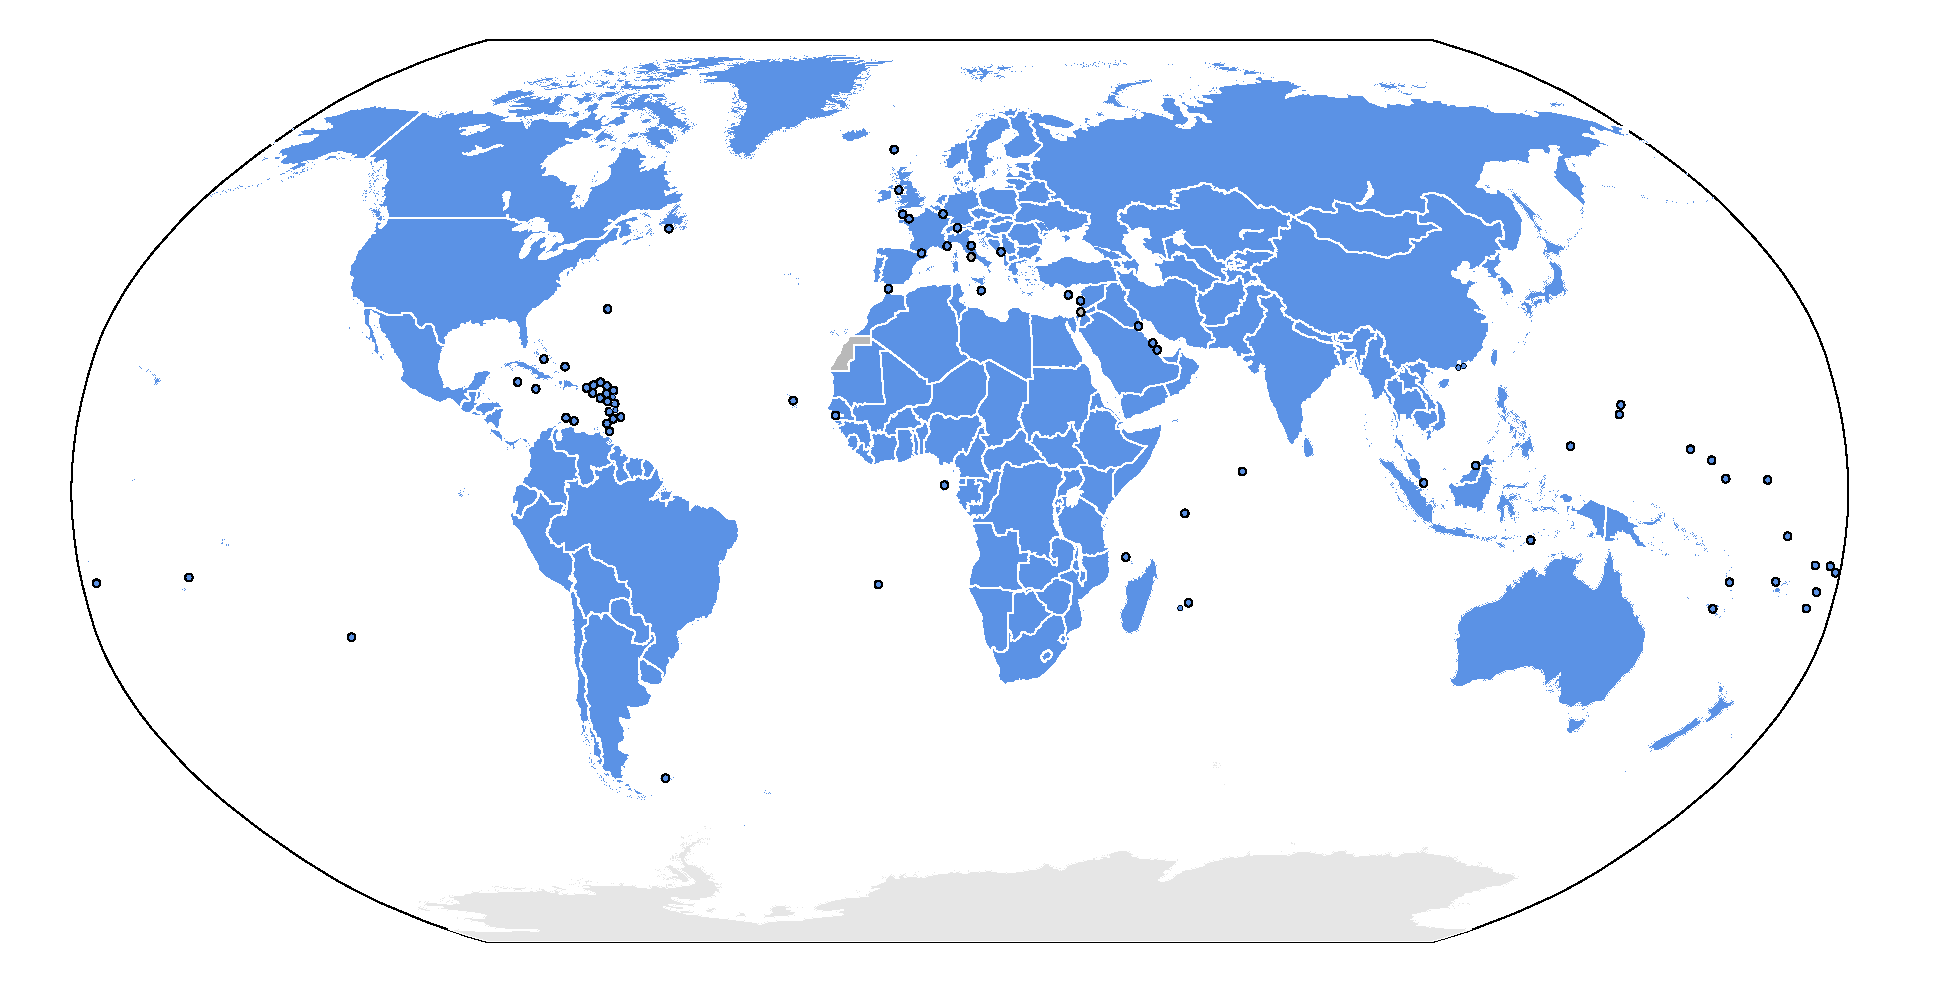
\includegraphics[width=8cm]{UN.pdf}
\caption{\footnotesize{Map showing the member states of the United Nations.}\label{fun}}
\end{center}
\end{figure}

\subsection{Dataset Preprocessing}
As noted by \cite{Huang2009} PCA might have troubles with variables which include big outliers, because in the normalization process, the mean of the sample resides far from both the majority of observations and the outliers. To bolster this issue, several strategies have been proposed, in particular, to make new synthetic variables taking the log of the original variables reducing the skewness. This was made for all non-negative variables spanning several orders of magnitude which were heavily left skewed, as shown in figure \ref{fig1}. This can also help to densify the center of mass of the observations. The previous claim was proved experimentally as shown in the figure \ref{fig2}. 
\begin{figure}[!ht]
\begin{center}
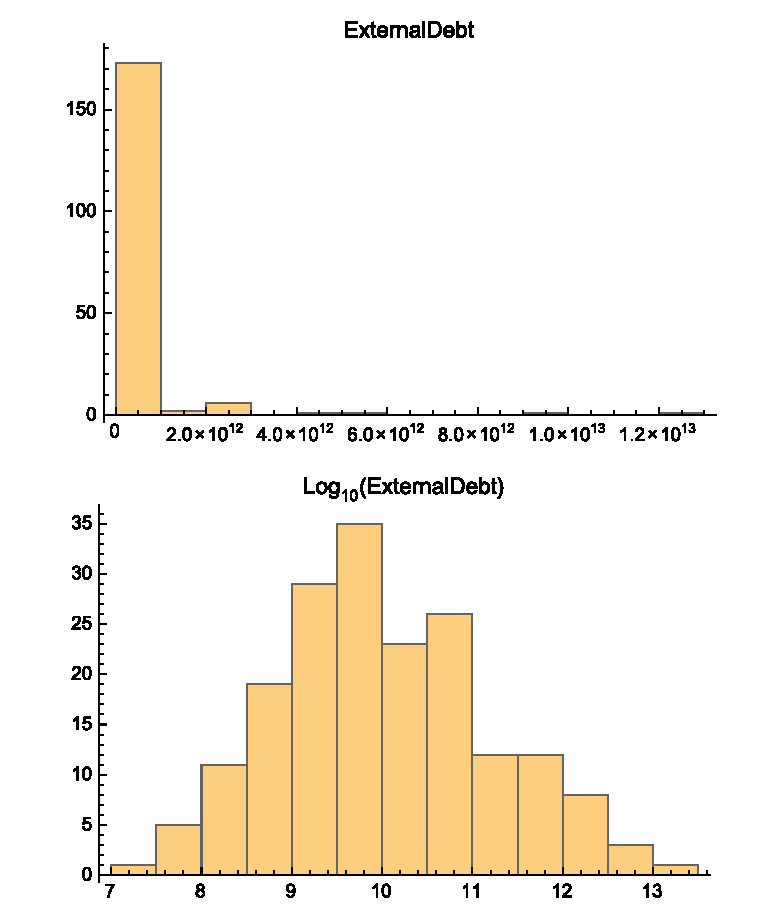
\includegraphics[width=8cm]{f1.eps}
\caption{\footnotesize{Histogram of the heavily skewed variables that span several orders of magnitude where treated taking the $\log_{10}$ to reduce the skewness as a measure of robustness. As seen in the figure, the new synthetic variable has a distribution closer to the Normal. The skewness goes from 6.73 to 0.31 respectively}\label{fig1}}
\end{center}
\end{figure}

Code for the querying and preprocessing transformations can be found in the appendix \ref{ap01}.

%\section{Exploratory Analysis}
%Some basic statistics were computed for the variables, in order to comprehend they range, mean, etc. Here are presented some notable cases.
%

\section{Data processing}
The resultant file \texttt{s1.xls} was imported to a licensed copy of \texttt{COHERIS SPAD} version \texttt{8.2.18}. The general schema of the process diagram is showed on figure \ref{schema}. 

\begin{figure}[!ht]
\begin{center}
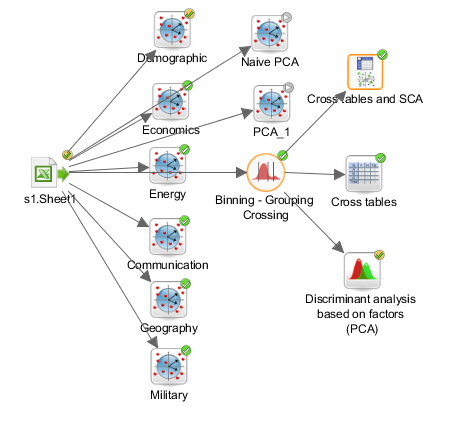
\includegraphics[width=8cm]{schema.png}
\caption{\footnotesize{General process diagram of the analysis. In the first stage six different PCA were carried out as exploratory analysis. Then a PCA analysis was done in a subset of the continuous variables, a CA was made after binding modalities on two variables and a FDA on factors to explain a categorical variable.}\label{schema}}
\end{center}
\end{figure}

First some descriptive statistics, and several %\footnote{A thing to note here is that no significance analysis, or quality of representation analysis of the factors was made in the exploratory analysis} 
normed PCA analysis on the different groups of variables was made as exploratory analysis. Then a normed PCA of the selected continuous variables was carried out to reduce the dimensionality of the dataset. Also a CA was made for two categorical variables to explore the relation between the continent and the economic sector, and finally a FDA was made to predict the economic sector based on the continuous variables. 

\subsection{Exploratory PCA}
Since the data is composed of 84 continuous variables, a more extensive approach was taken with the PCA method. Namely, exploring each group of variables separately as exploratory analysis to give some insight in the nature of the variables of each group. The categorical variable \texttt{Continent} has frequencies as showed in figure \ref{pie1} . 

\begin{figure}[!ht]
\begin{center}
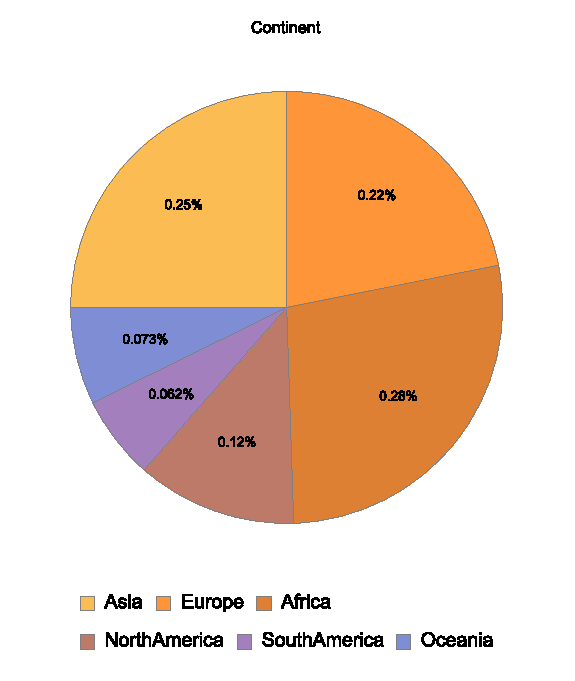
\includegraphics[width=6cm]{f21.eps}
\caption{\footnotesize{The total of 193 countries being studied are distributed amongst their respective continents as showed in the chart. }\label{pie1}}
\end{center}
\end{figure} 

\subsubsection{Demographics}

A normed PCA of the \texttt{Demographic} group of variables was carried out leading to the results shown in figure \ref{p1}. Around 73\% of the total inertia can be explained in the first two factors. There exists a high correlation between variables such as: \texttt{Poverty Fraction}, \texttt{Birth Rate Fraction}, \texttt{Total Fertitility Rate}, \texttt{Population Growth} and \texttt{Infant Mortality Fraction}. Group which is in contraposition with the highly correlated variables: \texttt{Literacy Fraction}, \texttt{Life Expectancy} and \texttt{Median Age}. A group of correlated variables stays in perpendicular relation with these contraposition and is composed of the variables \texttt{Annual Births}, \texttt{Child Population}, \texttt{Population}, \texttt{Annual Deaths}, \texttt{Adult Population} and \texttt{Elderly Population}. %The variables \texttt{Death Rate Fraction}  and \texttt{Migration Rate Fraction} are misrepresented since they contain several missing values. 
%The first factor contains, in the positive direction, high population, the second factor contains, in the positive direction, high birth rate and high poverty fraction.

When we plot the observations in this factors we can see that countries such as \texttt{NG: Federal Republic of Nigeria}, \textsc{NE: Republic of Niger}, \textsc{TD: Republic of Chad} lead the first quadrant\footnote{in the geometric sense}, that is the one associated  with high \texttt{Poverty Fraction}, high \texttt{Birth Rate Fraction}, etc. In the second quadrant countries such as \textsc{NR: Republic of Nauru}, \textsc{TV: Tuvalu} and \textsc{PW: Republic of Palau} all three in \textsc{Oceania} lead, that is they can be characterized by low \texttt{Annual Births} and \texttt{Population}. In the third quadrant we find countries such as \textsc{AT: Republic of Austria}, \textsc{DE: Federal Republic of Germany} and \textsc{GB: United Kingdom of Great Britain and Northern Ireland} that are characterized by high \texttt{Literacy Fraction}, high \texttt{Life Expectancy}, low \texttt{Poverty Fraction} and \texttt{Population Growth}. In the fourth quadrant we find countries such as \textsc{IN: Republic of India}, \textsc{CN: People's Republic of China} and \textsc{ID: 	Republic of Indonesia} which are characterized by high \texttt{Population}, high \texttt{Elderly Population} , \texttt{Annual Births} and \texttt{Annual Deaths}.

The \texttt{continent} has been plotted as a supplementary variable, showing that \textsc{Africa} is located in the first quadrant, \textsc{Oceania}  and \textsc{North America} in the second, \textsc{Europe} and \textsc{South America} in the third and \textsc{Asia} in the fourth. A thing to note is the position of the member of the \textsc{G8}\footnote{Group of the eight most industrialized countries: \textsc{FR, DE, JP, GB, US, CA, IT} and \textsc{RU}}, as a representative of the world dominance, we observe that they are grouped around the second factor negative direction, that is, demographically speaking, countries with high \texttt{Population}, high \texttt{Life Expectancy} and \texttt{Literacy Fraction} but still low \texttt{Poverty Fraction}, \texttt{Total Fertitility Rate} and \texttt{Population Growth}.

\subsubsection{Economics}
A normed PCA of the \texttt{Economic} group of variables was carried out leading to the results shown in the figure \ref{p2}. Around 58\% of the total inertia can be explained in the first two factors. There exists a high correlation between the variables: \texttt{GDP}, \texttt{GDP At Parity}, \texttt{Government Receipts}, \texttt{Government Expenditures}, \texttt{Government Debt}, \texttt{Foreign Exchange Reserves}, \texttt{External Debt}, this correlation is also very high with the first factor in the positive direction. Also the variables \texttt{GDP Real Growth}, \texttt{Industrial Production Growth} and \texttt{Exchange Rate} are highly correlated between each other and also to the second factor in the positive direction. The variable\texttt{Labor Force} is in the first quadrant, as a combination of the first and second factor in the positive direction, also the variable \texttt{GDP Per Capita} is in the fourth quadrant as a combination but  in the negative direction of the second factor, and the variable \texttt{Unemployment Fraction} is in contrapositive with \texttt{Unemployment Fraction}. % The variables \texttt{Inflation Rate} and \texttt{Price Index} are misrepresented because they contain several missing values.  

When we plot the observations in the factor plane we can see that, in the first factor, the countries with highest values are: \textsc{US: United States of America}, \textsc{JP: Japan}, \textsc{DE: Federal Republic of Germany}, \textsc{FR: French Republic}, that is, countries with high \texttt{GDP}, \texttt{External Debt} and both \texttt{Government Receipts}, \texttt{Government Expenditures}, \texttt{Government Debt}, \texttt{Government Expenditures}. Contrary to this, countries with the most negative value in the first factor \textsc{NR: Republic of Nauru} , \textsc{KI: Republic of Kiribati}, and \textsc{TO: Kingdom of Tonga} in \textsc{Oceania}. In the second factor, the countries with the most positive value are: \textsc{ET: Federal Democratic Republic of Ethiopia}, \textsc{AO: Republic of Angola}, \textsc{TZ: United Republic of Tanzania} in \textsc{Africa}. And in the opposite direction we have \textsc{LU: Grand Duchy of Luxembourg}, \textsc{EE: Republic of Estonia}, \textsc{IS: Iceland}. 

The \texttt{Continent} and the \texttt{Sector Labor Fractions} has been plotted as supplementary variables, showing that \textsc{Europe} has the highest value in the first factor, still keeping negative value in the second, whereas \textsc{Asia} and \textsc{South America} have both high value in both factors, \textsc{Africa} is in the second quarter and \textsc{North America} and \textsc{Oceania} have both negative values in the first and second factor. The \texttt{Sector Labor Fractions} \textsc{Services} is in the fourth quadrant, close to \textsc{Industry}, \textsc{Agriculture} is in the second quarter, and \textsc{Industry And Services} is in the third quarter. A thing to note is the locus of the countries members of \textsc{G8}, seven out of 8 remain really close, apart from anyone else, in the fourth quadrant, that is with high \texttt{External Debt}, \texttt{GDP}, and the highest \texttt{GDP Per Capite} but low \texttt{Exchange Rate}, \texttt{GDP Real Growth}, \texttt{Industrial Production Growth} and low \texttt{Unemployment Fraction}.

\subsubsection{Energy}
A normed PCA of the \texttt{Energy} group of variables was carried out leading to the results shown in the figure \ref{p3}. 

Around 56\% of the total inertia can be explained in the first two factors. There exists a high correlation between the variables: \texttt{Oil Imports}, \texttt{Oil Consumption}, \texttt{Electricity Production}, \texttt{Electricity Consumption}, and \texttt{Electricity Imports} in the first quadrant. Also the variables \texttt{Natural Gas Reserves}, \texttt{Oir Reserves}, \texttt{Natural Gas Production} and \texttt{Oil Production} are highly correlated between each other in the fourth quadrant. The variables \texttt{Oil Exports} and \texttt{Natural Gas Consumption} are also situated in the fourth quadrant. 

When we plot the observations in this factorial plane we can see that \textsc{US: United States of America} is far from any other observation with the highest value in the first factor, that is a combination of \texttt{Oil Imports}, \texttt{Oil Consumption}, \texttt{Electricity Production}, \texttt{Electricity Consumption}, \texttt{Electricity Imports}, \texttt{Natural Gas Reserves}, \texttt{Oil Reserves}, \texttt{Natural Gas Production} and \texttt{Oil Production} . Countries in the first quadrant, that is associated with \texttt{Oil Consumption}, \texttt{Electricity Imports}, \texttt{Electricity Consumption} and \texttt{Electricity Production}: \textsc{ES: Kingdom of Spain}, \textsc{FR: French Republic}, \textsc{IT: Italian Republic}, \textsc{JP: Japan}. In the other hand, countries situated in the fourth quadrant, that is associated with \texttt{Natural Gas Reserves}, \texttt{Oir Reserves}, \texttt{Natural Gas Production} and \texttt{Oil Production}: \textsc{RU: Russian Federation}, \textsc{IR: Islamic Republic of Iran} and \textsc{CA: Canada}. Countries close to the First factor, that is in a positive combination of the previous two groups are as previously mentioned, \textsc{US}, \textsc{GB} and \textsc{IN}. We must not forget that with synthetic logarithmic variables, now every distance in the play represents orders of magnitude, thus, the outlier \textsc{US} has significantly more energy consumption, production and trading that any other country.  On the contrary, the country closer to the first factor axis but with negative coordinates is \textsc{SL: Republic of Sierra Leone} that is, with the less energy consumption, production and trading. 

%The \texttt{Continent} variable is plotted a supplementary variable. We see that \textsc{Europe} appears in the first quadrant, \textsc{Africa, Oceania} and \textsc{North America} in the third quadrant and both \textsc{South America} and \textsc{Asia} in the fourth quadrant. 
If we pay attention to the members of the \textsc{G8} we see \textsc{US, CA, RU} in the fourth quadrant, that is of Oil producers, and the remaining \textsc{GB, DE, JP, IT, FR} of Oil importers and Electricity Producers. But still both are in the positive to far positive side of the First factor.

\subsubsection{Communication}
A normed PCA of the \texttt{Communication} group of variables was carried out leading to the results shown in the figure \ref{p4}. 

Around 65\% of the total inertia can be explained in the first two factors. There exists a high correlation between the variables: \texttt{Airports}, \texttt{Television Stations}, \texttt{Internet Users}, \texttt{AM/FM Radio Stations}, and \texttt{Road Length} with each other and with the first factor. Also the variables \texttt{Merchant Ships}, \texttt{Merchant Ships Dead Weight} and \texttt{Merchant Ships Gross} are highly correlated between each other in the fourth quadrant. 

When we plot the observations in this factorial plane we can see that \textsc{US: United States of America} is far from any other observation with the highest value in the first factor, followed by \textsc{BR: Federative Republic of Brazil}, \textsc{RU}, \textsc{CN}, \textsc{MX}, that is with high volume of land and radio communications. Countries with high values in the sector factor: \textsc{PA: Republic of Panama}, \textsc{LR: Republic of Liberia} that is with high values in Merchant Ships.

%The \texttt{Continent} variable is plotted a supplementary variable. We see that \textsc{Europe, Asia, North America} appear in the fourth quadrant, \textsc{South America} in the first quadrant, \textsc{Africa} in the second and \textsc{Oceania}  in the third quadrant. 
If we pay attention to the members of the \textsc{G8} we see \textsc{US} in the far positive factor, that is with high values in communication infrastructure, the remaining members remain close to each other with high values in the first factor.

\subsubsection{Geography}
A normed PCA of the \texttt{Geography} group of variables was carried out leading to the results shown in the figure \ref{p5}. 

Around 57\% of the total inertia can be explained in the first two factors. There exists a high correlation between the variables: \texttt{Area}, \texttt{Water Area}, \texttt{Boundary Length}, \texttt{Coastline Length}, and \texttt{Arable Land Area} with each other and with the first factor. Also the variables \texttt{Irrigated Land Fraction} and \texttt{Arable Land Fraction}  are highly correlated between each other in the negative direction of the second factor. There exist opposition by the variable \texttt{Lowest Elevation} in this second factor. And the variables \texttt{Crops Land Area} and \texttt{Irrigated Land Area} are correlated and in the fourth quadrant. 

When we plot the observations in this factorial plane we can see that \textsc{US, CA, RU, CN, IN} have the highest values in the first factor, that is related with the size of the country. In the negative direction of the second factor we find \textsc{MD: Republic of Moldova}  with high values in the \texttt{Arable Land Fraction} and \texttt{Irrigated Land Fraction}. On the other hand, countries with low values in the first factor are \textsc{MC	Principality of Monaco}, \textsc{VC	Saint Vincent and the Grenadines}, \textsc{BB: Barbados
} that is, small countries.


%The \texttt{Continent} variable is plotted a supplementary variable. We see that \textsc{Europe, Asia, North America} appear in the fourth quadrant, \textsc{South America} in the first quadrant, \textsc{Africa} in the second and \textsc{Oceania}  in the third quadrant. 
If we pay attention to the members of the \textsc{G8} we see \textsc{US, CA, RU} in the far positive factor, that is with high values in size the remaining members remain close to each other with not that high values in the first factor.

\subsubsection{Military}

A normed PCA of the \texttt{Military} group of variables was carried out leading to the results shown in the figure \ref{p6}. 

Around 79\% of the total inertia can be explained in the first two factors. There exists a high correlation between the variables: \texttt{Military Fit Population}, \texttt{Military Age Rate} and \texttt{Military Age Males} with each other and with the first factor. Also the variable \texttt{Military Expenditure Fraction} is highly correlated with the second factor. And the variable \texttt{Military Expenditure} is  in the first quadrant. 

When we plot the observations in this factorial plane we can see that \textsc{CN, IN, US} have the highest values in the first factor, that is related with the \texttt{Military Fit Population} of the country. In the negative direction of the second factor we find \textsc{ST: Democratic Republic of Sao Tome and Principe}. On the other hand, countries with high values in the second factor are \textsc{OM: Sultanate of Oman} and \textsc{QA	State of Qatar},  that is, with high values in \texttt{Military Expenditure Fraction}.


%The \texttt{Continent} variable is plotted a supplementary variable. We see that \textsc{Europe, Asia, North America} appear in the fourth quadrant, \textsc{South America} in the first quadrant, \textsc{Africa} in the second and \textsc{Oceania}  in the third quadrant. 
If we pay attention to the members of the \textsc{G8} we see \textsc{US, CA, RU} in the far positive factor, that is with high values in \texttt{Military Fit Population}  the remaining members remain close to each other with not that high values in the first factor.

\subsection{PCA}

Having explored these groups a variables, a normed PCA was made selecting 16 active variables, namely: \texttt{Life Expectancy}, \texttt{Population}, \texttt{Population Growth}, \texttt{Total Fertility Rate} in the \textsc{Demographics};  \texttt{Foreign Exchange Reserves}, \texttt{GDP}, \texttt{GDP Per Capita}, and \texttt{Labor Force} in the \textsc{Economics}; \texttt{Electricity Production}, and \texttt{Oil Exports} in the \textsc{Energy}; \texttt{Airports}, \texttt{Internet Hosts} and \texttt{Road Length} in the \textsc{Communication}; \texttt{Arable Land Area} and \texttt{Area} in the \textsc{Geography} and \texttt{Military Expenditures} and \texttt{Military Fit Population} in the \textsc{Military}. All the other variables are used as supplementary.  

The results of the test are shown in appendix \ref{pca} and figures are shown in the appendix \ref{r1}. 

Around 54.11\% of the inertia is captured by the first factor and 22.93\% by the second, that is a total of 77.04\% is captured by the first two factors. The first factor is mainly composed, in decreasing order by: \texttt{GDP}, \texttt{Military Fit Population}, \texttt{Internet Users}, \texttt{Road Length}, \texttt{Electricity Production}, \texttt{LaborForce} and \texttt{Population} all with positive correlation. And the second factor is mainly composed by \texttt{Total Fertility Rate} with positive correlation, and \texttt{GDP per Capita} and \texttt{Life Expectancy} with negative correlation. Thus there exist contraposition between these variables. 
The third factor is mainly composed by \texttt{Oil Exports} with negative correlation and the fourth factor by \texttt{Airports} also with negative correlation. 

When we plot the active cases we can observe in red, the countries members of the \textsc{G8}\footnote{\textsc{US	United States of America, RU	Russian Federation, CA	Canada, JP	Japan, DE	Federal Republic of Germany, FR	French Republic, GB	United Kingdom of Great Britain and Northern Ireland, IT	Italian Republic}} of the most industrialized countries are far to the right, where the \textsc{US} leads, followed by \textsc{RU} the remaining ones are close to each other in the fourth quadrant. Interestingly enough, the members of the \textsc{G5}\footnote{\textsc{CN	People's Republic of China, IN	Republic of India, BR	Federative Republic of Brazil, MX	United Mexican States, ZA	Republic of South Africa}}, in purple, of the emergent economies also are far to the right, close to each other, but closer to the first quadrant, that is with more value in the second factor. An interesting case is that recently \textsc{RU} has been banned from the \textsc{G8} as a consequence of the Ukrainian crisis and it's the farthest member of the \textsc{G8} in the second factor. The members of the \textsc{G10}\footnote Members of the IMF council {\textsc{NL	Kingdom of the Netherlands, SE	Kingdom of Sweden, BE	Kingdom of Belgium, CH	Swiss Confederation}} which are not members of the \textsc{G8} are shown also together, with less value in the first factor, but still more value in the negative direction of the second factor. 

As extreme cases, we may note, the \textsc{US} with the most positive value in the first factor, in the other side \textsc{ST	Democratic Republic of Sao Tome and Principe} with the most negative value. With the most positive value in the second factor \textsc{NE	Republic of Niger} and \textsc{CD	Democratic Republic of the Congo} and with the most negative value \textsc{SG	Republic of Singapore}, \textsc{LI	Principality of Liechtenstein}, \textsc{MC	Principality of Monaco}, \textsc{SM	Republic of San Marino} and \textsc{AD	Principality of Andorra}. 

\subsection{CA}

A Correspondence Analysis was carried out between two synthetic categorical variables, fabricated binding previous natural variables to assure nonzero frequencies in the contingency table. The modalities \textsc{Industry, Industry And Services, Services} from the variable \texttt{Sector Labor Fractions} where bound as \textsc{Industry And Services} and the modalities \textsc{North America} and \textsc{South America} where bound as \textsc{America}. A transcript of the printout can be found in \ref{ca} and a figure of the result can be found in appendix \ref{r2}.

In the independence test a $\chi^2$ of $75.01$ with a expected $\chi_4^2$ with four degrees of freedom with value $9.48773$ thus we reject the null hypothesis of the independence and we conclude there exists relation between the two categorical variables. 

The results show a relation between \texttt{Continents} \textsc{Europe, America} with \texttt{Sector Labor Fractions} \textsc{Industry And Services}, and also relation between \textsc{Africa} and \textsc{Agriculture} in the only factor. 


\subsection{FDA}

A Factorial Discriminant Analysis based on Factors was carried out to explain and predict the value of the categorical value \texttt{Sector Labor Fractions}. The same variables used in the PCA where used as explanatory variables. The results can be seen in the printout \ref{fda}.

The first two factors explain 95\% of the total inertia. The first factor is composed with negative correlation $-1.00$ by the variable \texttt{Life Expectancy} followed by \texttt{Total Fertility Rate} with positive correlation. The second factor is composed mostly by \texttt{Military Fit Population} and \texttt{Labor Force} with negative correlation. 

The confusion matrix shows a 85\% of well classified cases. The first factor has a high discriminant function and the model is significant with $0.000$ risk. Also in terms of the original variables, the most discriminant variables is \texttt{Life Expectancy}

%\section{Data postprocessing}

\section{Interpretations}

Trying to answer the firstly posed question \emph{What makes the wealth of a country?} we may say: Taking the group of \textsc{G8} as the ground truth for wealthy countries, that is, abundant of resources, with good quality of life, with international hegemony and influence, strong currencies, powerful armies, etc. We see all this elements effectively combined in the PCA study, saying: Wealthy countries have, high GDP, Electricity Production, Foreign Exchange Reserves, also they expend the most in Military and export Oil if any. They have high Life Expectancy and GDP per Capita, and this is may be the few variables related to people rather than macroeconomy, that is, in wealthy countries, people live more and they have more money, in wealthy countries, people are wealthy. This comes with a draw back of being in direct contraposition with the Total Fertility Rate, that is, in wealthy countries people have less kids. 

Also something to note is that members of the \textsc{G5} are similar to those of the \textsc{G8} in macro variables such as GDP, Electricity Production, etc, but they also tend to have more population, area and arable land area, also more total fertility rate, still some less life expectancy and GDP per capita. 

This draws important hypothesis. \emph{the amount of wealth is fixed, and is distributed amongst the citizens}. Countries with high wealth but high population are perceived as poor because their lack of GDP per capita, and more wealthy countries have less population and less children per women, still more GDP per capita.

Also an interesting point to draw is the opportunity for other countries to enter the international hegemony based on their current wealth, this is the case of \textsc{KR	Republic of Korea}, \textsc{ES	Kingdom of Spain}, \textsc{AU	Commonwealth of Australia}, \textsc{TR	Republic of Turkey}, \textsc{PL	Republic of Poland}, \textsc{SA	Kingdom of Saudi Arabia}, \textsc{IR	Islamic Republic of Iran}, \textsc{AR	Argentine Republic}, \textsc{MY	Malaysia}, \textsc{VE	Bolivarian Republic of Venezuela} and \textsc{TH	Kingdom of Thailand} which are close in the factor plane and thus have all the measured components of a wealthy country but still lack to have dominance in the international realm, may be just for lack of political will or strength.

The line that divides \textsc{G8} from \textsc{G5} seems to be the line of demography, one may say that a country is for it's children to come, so, one may say that the current \textsc{G5} will be the tomorrow's \textsc{G8} members based on the aging of the population. 

Using CA we were able to describe the relation between the economic activity and the continent of the country. That is, countries of the European and American continent are related to the Industry and Services activity, whereas African countries are related to Agricultural activities. 

Also using FDA we may say that the most discriminant variable to explain a countries activity is, by far, the Life Expectancy. And with this you can predict up to 85\% of the observations. 

\bibliography{/Users/Poincare/Dropbox/Tex/library.bib}
\bibliographystyle{unsrt}

\appendix
\onecolumn
\section{Appendices}
\subsection{Dataset Description}\label{ap001}
\begin{longtable}{cccc}
 \textbf{Index} & \textbf{Property} & \textbf{Unit} & \textbf{Group} \\
 1 & \text{CountryCode} & \text{None} & \text{Identification} \\
 2 & \text{FullName} & \text{None} & \text{Identification} \\
 3 & \text{Continent} & \text{None} & \text{Identification} \\
 4 & \text{IndependenceYear} & \text{None} & \text{Demographic} \\
 5 & \text{AdultPopulation} & \text{People} & \text{Demographic} \\
 6 & \text{AnnualBirths} & \text{PeoplePerYear} & \text{Demographic} \\
 7 & \text{AnnualDeaths} & \text{PeoplePerYear} & \text{Demographic} \\
 8 & \text{BirthRateFraction} & \text{PeoplePerPersonPerYear} & \text{Demographic} \\
 9 & \text{ChildPopulation} & \text{People} & \text{Demographic} \\
 10 & \text{DeathRateFraction} & \text{PeoplePerPersonPerYear} & \text{Demographic} \\
 11 & \text{ElderlyPopulation} & \text{People} & \text{Demographic} \\
 12 & \text{InfantMortalityFraction} & \text{PeoplePerPerson} & \text{Demographic} \\
 13 & \text{LifeExpectancy} & \text{Years} & \text{Demographic} \\
 14 & \text{LiteracyFraction} & \text{PeoplePerPerson} & \text{Demographic} \\
 15 & \text{MedianAge} & \text{Years} & \text{Demographic} \\
 16 & \text{MigrationRateFraction} & \text{PeoplePerPersonPerYear} & \text{Demographic} \\
 17 & \text{Population} & \text{People} & \text{Demographic} \\
 18 & \text{PopulationGrowth} & \text{PeoplePerPersonPerYear} & \text{Demographic} \\
 19 & \text{PovertyFraction} & \text{None} & \text{Demographic} \\
 20 & \text{TotalFertilityRate} & \text{PeoplePerPerson} & \text{Demographic} \\
 21 & \text{CurrencyCode} & \text{None} & \text{Economic} \\
 22 & \text{ExchangeRate} & \text{PerUSDollar} & \text{Economic} \\
 23 & \text{ExternalDebt} & \text{USDollars} & \text{Economic} \\
 24 & \text{ForeignExchangeReserves} & \text{USDollars} & \text{Economic} \\
 25 & \text{GDP} & \text{USDollarsPerYear} & \text{Economic} \\
 26 & \text{GDPAtParity} & \text{USDollarsPerYear} & \text{Economic} \\
 27 & \text{GDPPerCapita} & \text{USDollarsPerYearPerPerson} & \text{Economic} \\
 28 & \text{GDPRealGrowth} & \text{USDollarsPerYearPerYear} & \text{Economic} \\
 29 & \text{GovernmentDebt} & \text{USDollars} & \text{Economic} \\
 30 & \text{GovernmentExpenditures} & \text{USDollarsPerYear} & \text{Economic} \\
 31 & \text{GovernmentReceipts} & \text{USDollarsPerYear} & \text{Economic} \\
 32 & \text{IndustrialProductionGrowth} & \text{PerYear} & \text{Economic} \\
 33 & \text{InflationRate} & \text{PerYear} & \text{Economic} \\
 34 & \text{LaborForce} & \text{People} & \text{Economic} \\
 35 & \text{PriceIndex} & \text{None} & \text{Economic} \\
 36 & \text{UnemploymentFraction} & \text{None} & \text{Economic} \\
 37 & \text{SectorLaborFractions} & \text{None} & \text{Economic} \\
 38 & \text{ExportPartnersFractions} & \text{None} & \text{Economic} \\
 39 & \text{ImportPartnersFractions} & \text{None} & \text{Economic} \\
 40 & \text{ElectricityConsumption} & \text{KilowattHoursPerYear} & \text{Energy} \\
 41 & \text{ElectricityExports} & \text{KilowattHoursPerYear} & \text{Energy} \\
 42 & \text{ElectricityImports} & \text{KilowattHoursPerYear} & \text{Energy} \\
 43 & \text{ElectricityProduction} & \text{KilowattHoursPerYear} & \text{Energy} \\
 44 & \text{NaturalGasConsumption} & \text{CubicMetersPerYear} & \text{Energy} \\
 45 & \text{NaturalGasExports} & \text{CubicMetersPerYear} & \text{Energy} \\
 46 & \text{NaturalGasImports} & \text{CubicMetersPerYear} & \text{Energy} \\
 47 & \text{NaturalGasProduction} & \text{CubicMetersPerYear} & \text{Energy} \\
 48 & \text{NaturalGasReserves} & \text{CubicMeters} & \text{Energy} \\
 49 & \text{OilConsumption} & \text{BarrelsPerDay} & \text{Energy} \\
 50 & \text{OilExports} & \text{BarrelsPerDay} & \text{Energy} \\
 51 & \text{OilImports} & \text{BarrelsPerDay} & \text{Energy} \\
 52 & \text{OilProduction} & \text{BarrelsPerDay} & \text{Energy} \\
 53 & \text{OilReserves} & \text{Barrels} & \text{Energy} \\
 54 & \text{Airports} & \text{None} & \text{Communication} \\
 55 & \text{AMRadioStations} & \text{None} & \text{Communication} \\
 56 & \text{CellularPhones} & \text{None} & \text{Communication} \\
 57 & \text{FMRadioStations} & \text{None} & \text{Communication} \\
 58 & \text{InternetHosts} & \text{None} & \text{Communication} \\
 59 & \text{InternetUsers} & \text{People} & \text{Communication} \\
 60 & \text{MerchantShips} & \text{None} & \text{Communication} \\
 61 & \text{MerchantShipsDeadWeight} & \text{MetricTons} & \text{Communication} \\
 62 & \text{MerchantShipsGross} & \text{RegisterTons} & \text{Communication} \\
 63 & \text{PavedAirports} & \text{None} & \text{Communication} \\
 64 & \text{PhoneLines} & \text{None} & \text{Communication} \\
 65 & \text{RadioStations} & \text{None} & \text{Communication} \\
 66 & \text{RailwayLength} & \text{Kilometers} & \text{Communication} \\
 67 & \text{RoadLength} & \text{Kilometers} & \text{Communication} \\
 68 & \text{ShortWaveRadioStations} & \text{None} & \text{Communication} \\
 69 & \text{TelevisionStations} & \text{None} & \text{Communication} \\
 70 & \text{UnpavedAirports} & \text{None} & \text{Communication} \\
 71 & \text{ArableLandArea} & \text{SquareKilometers} & \text{Geography} \\
 72 & \text{ArableLandFraction} & \text{None} & \text{Geography} \\
 73 & \text{Area} & \text{SquareKilometers} & \text{Geography} \\
 74 & \text{BoundaryLength} & \text{Kilometers} & \text{Geography} \\
 75 & \text{CoastlineLength} & \text{Kilometers} & \text{Geography} \\
 76 & \text{CropsLandArea} & \text{SquareKilometers} & \text{Geography} \\
 77 & \text{CropsLandFraction} & \text{None} & \text{Geography} \\
 78 & \text{HighestElevation} & \text{Meters} & \text{Geography} \\
 79 & \text{IrrigatedLandArea} & \text{SquareKilometers} & \text{Geography} \\
 80 & \text{IrrigatedLandFraction} & \text{None} & \text{Geography} \\
 81 & \text{LandArea} & \text{SquareKilometers} & \text{Geography} \\
 82 & \text{LowestElevation} & \text{Meters} & \text{Geography} \\
 83 & \text{WaterArea} & \text{SquareKilometers} & \text{Geography} \\
 84 & \text{MilitaryAgeFemales} & \text{People} & \text{Military} \\
 85 & \text{MilitaryAgeMales} & \text{People} & \text{Military} \\
 86 & \text{MilitaryAgePopulation} & \text{People} & \text{Military} \\
 87 & \text{MilitaryAgeRate} & \text{PeoplePerYear} & \text{Military} \\
 88 & \text{MilitaryExpenditureFraction} & \text{None} & \text{Military} \\
 89 & \text{MilitaryExpenditures} & \text{USDollarsPerYear} & \text{Military} \\
 90 & \text{MilitaryFitPopulation} & \text{People} & \text{Military} \\
\end{longtable}
\newpage
\subsection{Countries Dictionary}\label{ap002}
\begin{longtable}{ccc}
 \text{AF} & \text{Islamic Republic of Afghanistan} & \text{Asia} \\
 \text{AL} & \text{Republic of Albania} & \text{Europe} \\
 \text{DZ} & \text{People's Democratic Republic of Algeria} & \text{Africa} \\
 \text{AD} & \text{Principality of Andorra} & \text{Europe} \\
 \text{AO} & \text{Republic of Angola} & \text{Africa} \\
 \text{AG} & \text{Antigua and Barbuda} & \text{NorthAmerica} \\
 \text{AR} & \text{Argentine Republic} & \text{SouthAmerica} \\
 \text{AM} & \text{Republic of Armenia} & \text{Asia} \\
 \text{AU} & \text{Commonwealth of Australia} & \text{Oceania} \\
 \text{AT} & \text{Republic of Austria} & \text{Europe} \\
 \text{AZ} & \text{Republic of Azerbaijan} & \text{Asia} \\
 \text{BS} & \text{Commonwealth of The Bahamas} & \text{NorthAmerica} \\
 \text{BH} & \text{Kingdom of Bahrain} & \text{Asia} \\
 \text{BD} & \text{People's Republic of Bangladesh} & \text{Asia} \\
 \text{BB} & \text{Barbados} & \text{NorthAmerica} \\
 \text{BY} & \text{Republic of Belarus} & \text{Europe} \\
 \text{BE} & \text{Kingdom of Belgium} & \text{Europe} \\
 \text{BZ} & \text{Belize} & \text{NorthAmerica} \\
 \text{BJ} & \text{Republic of Benin} & \text{Africa} \\
 \text{BT} & \text{Kingdom of Bhutan} & \text{Asia} \\
 \text{BO} & \text{Plurinational State of Bolivia} & \text{SouthAmerica} \\
 \text{BA} & \text{Bosnia and Herzegovina} & \text{Europe} \\
 \text{BW} & \text{Republic of Botswana} & \text{Africa} \\
 \text{BR} & \text{Federative Republic of Brazil} & \text{SouthAmerica} \\
 \text{BN} & \text{Brunei Darussalam} & \text{Asia} \\
 \text{BG} & \text{Republic of Bulgaria} & \text{Europe} \\
 \text{BF} & \text{Burkina Faso} & \text{Africa} \\
 \text{BI} & \text{Republic of Burundi} & \text{Africa} \\
 \text{KH} & \text{Kingdom of Cambodia} & \text{Asia} \\
 \text{CM} & \text{Republic of Cameroon} & \text{Africa} \\
 \text{CA} & \text{Canada} & \text{NorthAmerica} \\
 \text{CV} & \text{Republic of Cape Verde} & \text{Africa} \\
 \text{CF} & \text{Central African Republic} & \text{Africa} \\
 \text{TD} & \text{Republic of Chad} & \text{Africa} \\
 \text{CL} & \text{Republic of Chile} & \text{SouthAmerica} \\
 \text{CN} & \text{People's Republic of China} & \text{Asia} \\
 \text{CO} & \text{Republic of Colombia} & \text{SouthAmerica} \\
 \text{KM} & \text{Union of the Comoros} & \text{Africa} \\
 \text{CR} & \text{Republic of Costa Rica} & \text{NorthAmerica} \\
 \text{HR} & \text{Republic of Croatia} & \text{Europe} \\
 \text{CU} & \text{Republic of Cuba} & \text{NorthAmerica} \\
 \text{CY} & \text{Republic of Cyprus} & \text{Asia} \\
 \text{CZ} & \text{Czech Republic} & \text{Europe} \\
 \text{CD} & \text{Democratic Republic of the Congo} & \text{Africa} \\
 \text{DK} & \text{Kingdom of Denmark} & \text{Europe} \\
 \text{DJ} & \text{Republic of Djibouti} & \text{Africa} \\
 \text{DM} & \text{Commonwealth of Dominica} & \text{NorthAmerica} \\
 \text{DO} & \text{Dominican Republic} & \text{NorthAmerica} \\
 \text{TL} & \text{Democratic Republic of Timor-Leste} & \text{Asia} \\
 \text{EC} & \text{Republic of Ecuador} & \text{SouthAmerica} \\
 \text{EG} & \text{Arab Republic of Egypt} & \text{Africa} \\
 \text{SV} & \text{Republic of El Salvador} & \text{NorthAmerica} \\
 \text{GQ} & \text{Republic of Equatorial Guinea} & \text{Africa} \\
 \text{ER} & \text{State of Eritrea} & \text{Africa} \\
 \text{EE} & \text{Republic of Estonia} & \text{Europe} \\
 \text{ET} & \text{Federal Democratic Republic of Ethiopia} & \text{Africa} \\
 \text{FJ} & \text{Republic of the Fiji Islands} & \text{Oceania} \\
 \text{FI} & \text{Republic of Finland} & \text{Europe} \\
 \text{FR} & \text{French Republic} & \text{Europe} \\
 \text{GA} & \text{Gabonese Republic} & \text{Africa} \\
 \text{GM} & \text{Republic of The Gambia} & \text{Africa} \\
 \text{GE} & \text{Georgia} & \text{Asia} \\
 \text{DE} & \text{Federal Republic of Germany} & \text{Europe} \\
 \text{GH} & \text{Republic of Ghana} & \text{Africa} \\
 \text{GR} & \text{Hellenic Republic} & \text{Europe} \\
 \text{GD} & \text{Grenada} & \text{NorthAmerica} \\
 \text{GT} & \text{Republic of Guatemala} & \text{NorthAmerica} \\
 \text{GN} & \text{Republic of Guinea} & \text{Africa} \\
 \text{GW} & \text{Republic of Guinea-Bissau} & \text{Africa} \\
 \text{GY} & \text{Cooperative Republic of Guyana} & \text{SouthAmerica} \\
 \text{HT} & \text{Republic of Haiti} & \text{NorthAmerica} \\
 \text{HN} & \text{Republic of Honduras} & \text{NorthAmerica} \\
 \text{HU} & \text{Hungary} & \text{Europe} \\
 \text{IS} & \text{Iceland} & \text{Europe} \\
 \text{IN} & \text{Republic of India} & \text{Asia} \\
 \text{ID} & \text{Republic of Indonesia} & \text{Asia} \\
 \text{IR} & \text{Islamic Republic of Iran} & \text{Asia} \\
 \text{IQ} & \text{Republic of Iraq} & \text{Asia} \\
 \text{IE} & \text{Ireland} & \text{Europe} \\
 \text{IL} & \text{State of Israel} & \text{Asia} \\
 \text{IT} & \text{Italian Republic} & \text{Europe} \\
 \text{CI} & \text{Republic of Cote d'Ivoire} & \text{Africa} \\
 \text{JM} & \text{Jamaica} & \text{NorthAmerica} \\
 \text{JP} & \text{Japan} & \text{Asia} \\
 \text{JO} & \text{Hashemite Kingdom of Jordan} & \text{Asia} \\
 \text{KZ} & \text{Republic of Kazakhstan} & \text{Asia} \\
 \text{KE} & \text{Republic of Kenya} & \text{Africa} \\
 \text{KI} & \text{Republic of Kiribati} & \text{Oceania} \\
 \text{KW} & \text{State of Kuwait} & \text{Asia} \\
 \text{KG} & \text{Kyrgyz Republic} & \text{Asia} \\
 \text{LA} & \text{Lao People's Democratic Republic} & \text{Asia} \\
 \text{LV} & \text{Republic of Latvia} & \text{Europe} \\
 \text{LB} & \text{Lebanese Republic} & \text{Asia} \\
 \text{LS} & \text{Kingdom of Lesotho} & \text{Africa} \\
 \text{LR} & \text{Republic of Liberia} & \text{Africa} \\
 \text{LY} & \text{Great Socialist People's Libyan Arab Jamahiriya} & \text{Africa} \\
 \text{LI} & \text{Principality of Liechtenstein} & \text{Europe} \\
 \text{LT} & \text{Republic of Lithuania} & \text{Europe} \\
 \text{LU} & \text{Grand Duchy of Luxembourg} & \text{Europe} \\
 \text{MK} & \text{Republic of Macedonia (FYROM)} & \text{Europe} \\
 \text{MG} & \text{Republic of Madagascar} & \text{Africa} \\
 \text{MW} & \text{Republic of Malawi} & \text{Africa} \\
 \text{MY} & \text{Malaysia} & \text{Asia} \\
 \text{MV} & \text{Republic of Maldives} & \text{Asia} \\
 \text{ML} & \text{Republic of Mali} & \text{Africa} \\
 \text{MT} & \text{Republic of Malta} & \text{Europe} \\
 \text{MH} & \text{Republic of the Marshall Islands} & \text{Oceania} \\
 \text{MR} & \text{Islamic Republic of Mauritania} & \text{Africa} \\
 \text{MU} & \text{Republic of Mauritius} & \text{Africa} \\
 \text{MX} & \text{United Mexican States} & \text{NorthAmerica} \\
 \text{FM} & \text{Federated States of Micronesia} & \text{Oceania} \\
 \text{MD} & \text{Republic of Moldova} & \text{Europe} \\
 \text{MC} & \text{Principality of Monaco} & \text{Europe} \\
 \text{MN} & \text{Mongolia} & \text{Asia} \\
 \text{ME} & \text{Republic of Montenegro} & \text{Europe} \\
 \text{MA} & \text{Kingdom of Morocco} & \text{Africa} \\
 \text{MZ} & \text{Republic of Mozambique} & \text{Africa} \\
 \text{MM} & \text{Union of Myanmar} & \text{Asia} \\
 \text{NA} & \text{Republic of Namibia} & \text{Africa} \\
 \text{NR} & \text{Republic of Nauru} & \text{Oceania} \\
 \text{NP} & \text{Federal Democratic Republic of Nepal} & \text{Asia} \\
 \text{NL} & \text{Kingdom of the Netherlands} & \text{Europe} \\
 \text{NZ} & \text{New Zealand} & \text{Oceania} \\
 \text{NI} & \text{Republic of Nicaragua} & \text{NorthAmerica} \\
 \text{NE} & \text{Republic of Niger} & \text{Africa} \\
 \text{NG} & \text{Federal Republic of Nigeria} & \text{Africa} \\
 \text{KP} & \text{Democratic People's Republic of Korea} & \text{Asia} \\
 \text{NO} & \text{Kingdom of Norway} & \text{Europe} \\
 \text{OM} & \text{Sultanate of Oman} & \text{Asia} \\
 \text{PK} & \text{Islamic Republic of Pakistan} & \text{Asia} \\
 \text{PW} & \text{Republic of Palau} & \text{Oceania} \\
 \text{PA} & \text{Republic of Panama} & \text{NorthAmerica} \\
 \text{PG} & \text{Independent State of Papua New Guinea} & \text{Oceania} \\
 \text{PY} & \text{Republic of Paraguay} & \text{SouthAmerica} \\
 \text{PE} & \text{Republic of Peru} & \text{SouthAmerica} \\
 \text{PH} & \text{Republic of the Philippines} & \text{Asia} \\
 \text{PL} & \text{Republic of Poland} & \text{Europe} \\
 \text{PT} & \text{Portuguese Republic} & \text{Europe} \\
 \text{QA} & \text{State of Qatar} & \text{Asia} \\
 \text{CG} & \text{Republic of the Congo} & \text{Africa} \\
 \text{RO} & \text{Romania} & \text{Europe} \\
 \text{RU} & \text{Russian Federation} & \text{Asia} \\
 \text{RW} & \text{Republic of Rwanda} & \text{Africa} \\
 \text{KN} & \text{Federation of Saint Kitts and Nevis} & \text{NorthAmerica} \\
 \text{LC} & \text{Saint Lucia} & \text{NorthAmerica} \\
 \text{VC} & \text{Saint Vincent and the Grenadines} & \text{NorthAmerica} \\
 \text{WS} & \text{Independent State of Samoa} & \text{Oceania} \\
 \text{SM} & \text{Republic of San Marino} & \text{Europe} \\
 \text{ST} & \text{Democratic Republic of Sao Tome and Principe} & \text{Africa} \\
 \text{SA} & \text{Kingdom of Saudi Arabia} & \text{Asia} \\
 \text{SN} & \text{Republic of Senegal} & \text{Africa} \\
 \text{RS} & \text{Republic of Serbia} & \text{Europe} \\
 \text{SC} & \text{Republic of Seychelles} & \text{Africa} \\
 \text{SL} & \text{Republic of Sierra Leone} & \text{Africa} \\
 \text{SG} & \text{Republic of Singapore} & \text{Asia} \\
 \text{SK} & \text{Slovak Republic} & \text{Europe} \\
 \text{SI} & \text{Republic of Slovenia} & \text{Europe} \\
 \text{SB} & \text{Solomon Islands} & \text{Oceania} \\
 \text{SO} & \text{Somalia} & \text{Africa} \\
 \text{ZA} & \text{Republic of South Africa} & \text{Africa} \\
 \text{KR} & \text{Republic of Korea} & \text{Asia} \\
 \text{ES} & \text{Kingdom of Spain} & \text{Europe} \\
 \text{LK} & \text{Democratic Socialist Republic of Sri Lanka} & \text{Asia} \\
 \text{SD} & \text{Republic of the Sudan} & \text{Africa} \\
 \text{SR} & \text{Republic of Suriname} & \text{SouthAmerica} \\
 \text{SZ} & \text{Kingdom of Swaziland} & \text{Africa} \\
 \text{SE} & \text{Kingdom of Sweden} & \text{Europe} \\
 \text{CH} & \text{Swiss Confederation} & \text{Europe} \\
 \text{SY} & \text{Syrian Arab Republic} & \text{Asia} \\
 \text{TJ} & \text{Republic of Tajikistan} & \text{Asia} \\
 \text{TZ} & \text{United Republic of Tanzania} & \text{Africa} \\
 \text{TH} & \text{Kingdom of Thailand} & \text{Asia} \\
 \text{TG} & \text{Togolese Republic} & \text{Africa} \\
 \text{TO} & \text{Kingdom of Tonga} & \text{Oceania} \\
 \text{TT} & \text{Republic of Trinidad and Tobago} & \text{NorthAmerica} \\
 \text{TN} & \text{Tunisian Republic} & \text{Africa} \\
 \text{TR} & \text{Republic of Turkey} & \text{Asia} \\
 \text{TM} & \text{Turkmenistan} & \text{Asia} \\
 \text{TV} & \text{Tuvalu} & \text{Oceania} \\
 \text{UG} & \text{Republic of Uganda} & \text{Africa} \\
 \text{UA} & \text{Ukraine} & \text{Europe} \\
 \text{AE} & \text{United Arab Emirates} & \text{Asia} \\
 \text{GB} & \text{United Kingdom of Great Britain and Northern Ireland} & \text{Europe} \\
 \text{US} & \text{United States of America} & \text{NorthAmerica} \\
 \text{UY} & \text{Oriental Republic of Uruguay} & \text{SouthAmerica} \\
 \text{UZ} & \text{Republic of Uzbekistan} & \text{Asia} \\
 \text{VU} & \text{Republic of Vanuatu} & \text{Oceania} \\
 \text{VE} & \text{Bolivarian Republic of Venezuela} & \text{SouthAmerica} \\
 \text{VN} & \text{Socialist Republic of Vietnam} & \text{Asia} \\
 \text{YE} & \text{Republic of Yemen} & \text{Asia} \\
 \text{ZM} & \text{Republic of Zambia} & \text{Africa} \\
 \text{ZW} & \text{Republic of Zimbabwe} & \text{Africa} \\
\end{longtable}
\newpage
\subsection{Preprocessing Code}\label{ap01}
\begin{lstlisting}[language=Mathematica]
SetDirectory[NotebookDirectory[]]
(*Index of the Selected Variables *)
vars1 = {33, 84, 30, 111, 1, 8, 9, 14, 25, 41, 45, 114, 132, 133, 148,
    154, 187, 188, 189, 212, 36, 60, 66, 80, 87, 88, 89, 90, 94, 95, 
   96, 112, 116, 126, 190, 216, 202, 64, 108, 52, 53, 54, 55, 169, 
   170, 171, 172, 173, 176, 177, 178, 179, 180, 4, 7, 22, 79, 120, 
   121, 150, 151, 152, 182, 184, 191, 194, 199, 204, 208, 219, 11, 12,
    13, 17, 28, 34, 35, 100, 123, 124, 127, 134, 222, 155, 
   156, 157, 158, 159, 160, 163};
(*Prints the variable Map*)
Prepend[{Range[Length[vars1]], CountryData["Properties"][[vars1]], 
     CountryData["US", #, "Units"] & /@ 
      CountryData["Properties"][[vars1]]}\[Transpose], {"Index", 
    "Property", "Unit"}] // TableForm;
(*Retrieves the Selected variables of the countries of the United \
Nations from the Wolfram|Alpha Knowledge Base*)
s1 = Transpose[
   ParallelTable[
    CountryData[CountryData["UN"][[j]], 
     CountryData["Properties"][[i]]], {i, vars1}, {j, 
     Length[CountryData["UN"]]}]];
(*Converts Quantity objects to plain plain text*)
q1 = Flatten[
   Position[
    Table[AnyTrue[QuantityQ /@ (s1\[Transpose][[j]]), TrueQ], {j, 
      Length[s1\[Transpose]]}], True]];
For[ii = 1, ii <= Length[s1], ii++,
 s1[[ii, q1]] = QuantityMagnitude[s1[[ii, q1]]]
 ]
(*Takes the log base 10 of a subset of the selected variables*)
log = Complement[
   Range[Length[s1\[Transpose]]], {1, 2, 3, 21, 37, 38, 39}, {8, 10, 
    12, 13, 14, 15, 16, 18, 19, 20, 28, 32, 33, 35, 36, 72, 78, 80, 
    88}];
For[ii = 1, ii <= Length[log], ii++,
 s1[[All, notlog[[ii]]]] = Log[10, s1[[All, notlog[[ii]]]]]
 ]
(*Converts Entity Object to plain text*)
s1[[All, 3]] = CanonicalName[s1\[Transpose][[3]]];
s1[[All, 4]] = Map[Part[#, 1] &, Normal /@ s1[[All, 4]]];
s1[[All, 37]] = 
  Part[#, 1, 1] & /@ (Sort[#, #1[[2]] > #2[[2]] &] & /@ s1[[All, 37]]);
s1[[All, 38]] = 
  CanonicalName[
   Part[#, 1, 1] & /@ (Sort[#, #1[[2]] > #2[[2]] &] & /@ 
      s1[[All, 38]])];
s1[[All, 39]] = 
  CanonicalName[
   Part[#, 1, 1] & /@ (Sort[#, #1[[2]] > #2[[2]] &] & /@ 
      s1[[All, 39]])];
(*Signals correctly the missing Data for output*)
s1 = Replace[s1, 
   Missing["NotAvailable"][[1, 1]] -> Missing["NotAvailable"], 2];
s1 = Replace[s1, 
   CanonicalName[Missing["NotAvailable"][[1, 1]]] -> 
    Missing["NotAvailable"], 2];
s1 = Replace[s1, 
   QuantityMagnitude[Missing["NotAvailable"]] -> 
    Missing["NotAvailable"], 2];
s1 = Replace[s1, 
   QuantityMagnitude[Missing["NotApplicable"]] -> 
    Missing["NotAvailable"], 2];
s1 = Replace[s1, "NotApplicable" -> Missing["NotAvailable"], 2];
(*Removes undesired countries*)
s1 = Select[
   s1, ! IntersectingQ[{#[[1]]}, {"CX", "CC", "FK", 
       Missing["NotApplicable"], "NU", "NF", "PN", "SJ", "TK", "VA", 
       "WF", "SS"}] &];
(*Save binaries of the computation*)
s1 >> "s1.mx"
(*Retrieve the binaries*)
<< s1.mx;
(*Export to excel*)
Export["s1.xls", 
 Insert[s1, CountryData["Properties"][[vars1]], 1]]
\end{lstlisting}
\newpage
\begin{landscape}
\subsection{Printouts}
\subsubsection{PCA}\label{pca}
\begin{verbatim}
SELECTION OF CASES AND VARIABLES
SUPPLEMENTARY CATEGORICAL VARIABLES
     2 VARIABLES      11 ASSOCIATED CATEGORIES
----------------------------------------------------------------------------------------------------------------------------------
   2 . Continent                                                    (   6 CATEGORIES )
  35 . SectorLaborFractions                                         (   5 CATEGORIES )
----------------------------------------------------------------------------------------------------------------------------------
ACTIVE CONTINUOUS VARIABLES
    16 VARIABLES
----------------------------------------------------------------------------------------------------------------------------------
  11 . LifeExpectancy                                               ( CONTINUOUS )
  15 . Population                                                   ( CONTINUOUS )
  18 . TotalFertilityRate                                           ( CONTINUOUS )
  22 . ForeignExchangeReserves                                      ( CONTINUOUS )
  23 . GDP                                                          ( CONTINUOUS )
  25 . GDPPerCapita                                                 ( CONTINUOUS )
  32 . LaborForce                                                   ( CONTINUOUS )
  41 . ElectricityProduction                                        ( CONTINUOUS )
  48 . OilExports                                                   ( CONTINUOUS )
  52 . Airports                                                     ( CONTINUOUS )
  57 . InternetUsers                                                ( CONTINUOUS )
  65 . RoadLength                                                   ( CONTINUOUS )
  69 . ArableLandArea                                               ( CONTINUOUS )
  71 . Area                                                         ( CONTINUOUS )
  87 . MilitaryExpenditures                                         ( CONTINUOUS )
  88 . MilitaryFitPopulation                                        ( CONTINUOUS )
----------------------------------------------------------------------------------------------------------------------------------
SUPPLEMENTARY CONTINUOUS VARIABLES
    66 VARIABLES
----------------------------------------------------------------------------------------------------------------------------------
   3 . AdultPopulation                                              ( CONTINUOUS )
   4 . AnnualBirths                                                 ( CONTINUOUS )
   5 . AnnualDeaths                                                 ( CONTINUOUS )
   6 . BirthRateFraction                                            ( CONTINUOUS )
   7 . ChildPopulation                                              ( CONTINUOUS )
   8 . DeathRateFraction                                            ( CONTINUOUS )
   9 . ElderlyPopulation                                            ( CONTINUOUS )
  10 . InfantMortalityFraction                                      ( CONTINUOUS )
  12 . LiteracyFraction                                             ( CONTINUOUS )
  13 . MedianAge                                                    ( CONTINUOUS )
  14 . MigrationRateFraction                                        ( CONTINUOUS )
  16 . PopulationGrowth                                             ( CONTINUOUS )
  17 . PovertyFraction                                              ( CONTINUOUS )
  20 . ExchangeRate                                                 ( CONTINUOUS )
  21 . ExternalDebt                                                 ( CONTINUOUS )
  24 . GDPAtParity                                                  ( CONTINUOUS )
  26 . GDPRealGrowth                                                ( CONTINUOUS )
  27 . GovernmentDebt                                               ( CONTINUOUS )
  28 . GovernmentExpenditures                                       ( CONTINUOUS )
  29 . GovernmentReceipts                                           ( CONTINUOUS )
  30 . IndustrialProductionGrowth                                   ( CONTINUOUS )
  31 . InflationRate                                                ( CONTINUOUS )
  33 . PriceIndex                                                   ( CONTINUOUS )
  34 . UnemploymentFraction                                         ( CONTINUOUS )
  38 . ElectricityConsumption                                       ( CONTINUOUS )
  39 . ElectricityExports                                           ( CONTINUOUS )
  40 . ElectricityImports                                           ( CONTINUOUS )
  42 . NaturalGasConsumption                                        ( CONTINUOUS )
  43 . NaturalGasExports                                            ( CONTINUOUS )
  44 . NaturalGasImports                                            ( CONTINUOUS )
  45 . NaturalGasProduction                                         ( CONTINUOUS )
  46 . NaturalGasReserves                                           ( CONTINUOUS )
  47 . OilConsumption                                               ( CONTINUOUS )
  49 . OilImports                                                   ( CONTINUOUS )
  50 . OilProduction                                                ( CONTINUOUS )
  51 . OilReserves                                                  ( CONTINUOUS )
  53 . AMRadioStations                                              ( CONTINUOUS )
  54 . CellularPhones                                               ( CONTINUOUS )
  55 . FMRadioStations                                              ( CONTINUOUS )
  56 . InternetHosts                                                ( CONTINUOUS )
  58 . MerchantShips                                                ( CONTINUOUS )
  59 . MerchantShipsDeadWeight                                      ( CONTINUOUS )
  60 . MerchantShipsGross                                           ( CONTINUOUS )
  61 . PavedAirports                                                ( CONTINUOUS )
  62 . PhoneLines                                                   ( CONTINUOUS )
  63 . RadioStations                                                ( CONTINUOUS )
  64 . RailwayLength                                                ( CONTINUOUS )
  66 . ShortWaveRadioStations                                       ( CONTINUOUS )
  67 . TelevisionStations                                           ( CONTINUOUS )
  68 . UnpavedAirports                                              ( CONTINUOUS )

  70 . ArableLandFraction                                           ( CONTINUOUS )
  72 . BoundaryLength                                               ( CONTINUOUS )
  73 . CoastlineLength                                              ( CONTINUOUS )
  74 . CropsLandArea                                                ( CONTINUOUS )
  75 . CropsLandFraction                                            ( CONTINUOUS )
  76 . HighestElevation                                             ( CONTINUOUS )
  77 . IrrigatedLandArea                                            ( CONTINUOUS )
  78 . IrrigatedLandFraction                                        ( CONTINUOUS )
  79 . LandArea                                                     ( CONTINUOUS )
  80 . LowestElevation                                              ( CONTINUOUS )
  81 . WaterArea                                                    ( CONTINUOUS )
  82 . MilitaryAgeFemales                                           ( CONTINUOUS )
  83 . MilitaryAgeMales                                             ( CONTINUOUS )
  84 . MilitaryAgePopulation                                        ( CONTINUOUS )
  85 . MilitaryAgeRate                                              ( CONTINUOUS )
  86 . MilitaryExpenditureFraction                                  ( CONTINUOUS )
----------------------------------------------------------------------------------------------------------------------------------
CASES
----------------------------- NUMBER --------------WEIGHT ---------------
 WEIGHT OF CASES      : Weight of objects, uniform equal to 1.                  UNIF
 KEPT ............... NITOT =    192      PITOT =             192.000
 ACTIVE ............. NIACT =    192      PIACT =             192.000
 SUPPLEMENTARY ...... NISUP =      0      PISUP =               0.000
-------------------------------------------------------------------------

PRINCIPAL COMPONENTS ANALYSIS
SUMMARY STATISTICS OF CONTINUOUS VARIABLES
TOTAL COUNT    :     192             TOTAL WEIGHT   :     192.00
+-------------------------------------------------------+----------------------+----------------------+
| NUM . IDEN - LABEL                  COUNT     WEIGHT  |      MEAN  STD.DEV.  |   MINIMUM   MAXIMUM  |
+-------------------------------------------------------+----------------------+----------------------+
|  11 . Life - LifeExpectancy           192     192.00  |     70.37      8.93  |     45.56     83.58  |
|  15 . Popu - Population               192     192.00  |      6.23      1.01  |      3.00      9.00  |
|  18 . Tota - TotalFertilityRate       192     192.00  |      2.82      1.40  |      1.19      7.56  |
|  22 . Fore - ForeignExchangeReser     153     153.00  |      9.77      0.94  |      7.38     12.31  |
|  23 . GDP  - GDP                      192     192.00  |     10.36      1.08  |      7.39     13.15  |
|  25 . GDPP - GDPPerCapita             192     192.00  |      3.64      0.71  |      2.14      5.33  |
|  32 . Labo - LaborForce               185     185.00  |      5.88      0.98  |      3.00      8.00  |
|  41 . Elec - ElectricityProductio     184     184.00  |      9.83      1.16  |      7.15     12.62  |
|  48 . OilE - OilExports               128     128.00  |      4.17      1.32  |      1.00      6.00  |
|  52 . Airp - Airports                 188     188.00  |      1.15      0.78  |      0.00      4.00  |
|  57 . Inte - InternetUsers            190     190.00  |      5.35      1.09  |      2.00      8.00  |
|  65 . Road - RoadLength               192     192.00  |      3.83      1.00  |      0.00      6.00  |
|  69 . Arab - ArableLandArea           190     190.00  |      3.39      1.25  |      0.00      6.00  |
|  71 . Area - Area                     192     192.00  |      4.39      1.25  |      0.00      7.00  |
|  87 . Mili - MilitaryExpenditures     165     165.00  |      8.60      1.10  |      5.77     11.70  |
|  88 . Mili - MilitaryFitPopulatio     192     192.00  |      5.82      0.98  |      3.00      8.00  |
|-------------------------------------------------------|----------------------|-----------------------
|   3 . Adul - AdultPopulation          192     192.00  |      6.02      1.00  |      3.00      8.00  |
|   4 . Annu - AnnualBirths             192     192.00  |      4.51      1.03  |      2.00      7.00  |
|   5 . Annu - AnnualDeaths             192     192.00  |      4.15      1.06  |      1.00      7.00  |
|   6 . Birt - BirthRateFraction        192     192.00  |      0.02      0.01  |      0.01      0.09  |
|   7 . Chil - ChildPopulation          192     192.00  |      5.62      1.02  |      3.00      8.00  |
|   8 . Deat - DeathRateFraction        192     192.00  |      0.01      0.00  |      0.00      0.02  |
|   9 . Elde - ElderlyPopulation        192     192.00  |      5.02      1.08  |      2.00      8.00  |
|  10 . Infa - InfantMortalityFract     191     191.00  |      0.03      0.03  |      0.00      0.18  |
|  12 . Lite - LiteracyFraction         188     188.00  |      0.84      0.19  |      0.22      1.00  |
|  13 . Medi - MedianAge                182     182.00  |     27.56      8.38  |     15.09     44.86  |
|  14 . Migr - MigrationRateFractio     191     191.00  |      0.00      0.00  |     -0.02      0.02  |
|  16 . Popu - PopulationGrowth         192     192.00  |      0.01      0.01  |     -0.01      0.04  |
|  17 . Pove - PovertyFraction          139     139.00  |      0.32      0.19  |      0.04      0.86  |
|  20 . Exch - ExchangeRate             192     192.00  |      1.33      1.49  |     -0.57     12.44  |
|  21 . Exte - ExternalDebt             185     185.00  |     10.01      1.18  |      7.00     13.09  |
|  24 . GDPA - GDPAtParity              192     192.00  |     10.54      1.04  |      7.17     13.16  |
|  26 . GDPR - GDPRealGrowth            192     192.00  |      0.04      0.04  |     -0.15      0.16  |
|  27 . Gove - GovernmentDebt           127     127.00  |     10.26      0.94  |      8.25     12.91  |
|  28 . Gove - GovernmentExpenditur     189     189.00  |      9.08      1.19  |      7.00     12.00  |
|  29 . Gove - GovernmentReceipts       189     189.00  |      9.06      1.19  |      7.00     12.00  |
|  30 . Indu - IndustrialProduction     170     170.00  |      0.03      0.04  |     -0.15      0.14  |
|  31 . Infl - InflationRate            192     192.00  |      0.12      0.10  |     -0.19      0.52  |
|  33 . Pric - PriceIndex               192     192.00  |    188.32     71.41  |     67.30    410.74  |
|  34 . Unem - UnemploymentFraction     168     168.00  |      0.14      0.16  |      0.00      0.90  |
|  38 . Elec - ElectricityConsumpti     183     183.00  |      9.78      1.15  |      7.11     12.59  |
|  39 . Elec - ElectricityExports        81      81.00  |      8.67      1.15  |      5.00     10.00  |
|  40 . Elec - ElectricityImports        92      92.00  |      8.59      1.09  |      4.00     10.00  |
|  42 . Natu - NaturalGasConsumptio     106     106.00  |      9.18      0.97  |      7.00     11.00  |
|  43 . Natu - NaturalGasExports         43      43.00  |      9.23      0.96  |      7.00     11.00  |
|  44 . Natu - NaturalGasImports         63      63.00  |      9.14      0.81  |      7.00     11.00  |
|  45 . Natu - NaturalGasProduction      90      90.00  |      9.03      1.18  |      6.00     11.00  |
|  46 . Natu - NaturalGasReserves       100     100.00  |     11.05      1.18  |      7.43     13.65  |
|  47 . OilC - OilConsumption           182     182.00  |      4.19      1.04  |      2.00      7.00  |
|  49 . OilI - OilImports               180     180.00  |      4.10      0.98  |      2.00      7.00  |
|  50 . OilP - OilProduction            109     109.00  |      4.27      1.35  |      0.00      6.00  |
|  51 . OilR - OilReserves               96      96.00  |      8.22      1.36  |      5.00     11.00  |
|  53 . AMRa - AMRadioStations          171     171.00  |      0.63      0.77  |      0.00      3.00  |
|  54 . Cell - CellularPhones           191     191.00  |      5.94      1.08  |      2.00      8.00  |
|  55 . FMRa - FMRadioStations          182     182.00  |      0.87      0.77  |      0.00      3.00  |
|  56 . Inte - InternetHosts            191     191.00  |      3.74      1.83  |      0.00      8.00  |
|  58 . Merc - MerchantShips            148     148.00  |      1.05      0.88  |      0.00      3.00  |
|  59 . Merc - MerchantShipsDeadWei     143     143.00  |      5.01      1.31  |      2.00      8.00  |
|  60 . Merc - MerchantShipsGross       143     143.00  |      4.92      1.19  |      3.00      8.00  |
|  61 . Pave - PavedAirports            187     187.00  |      0.73      0.68  |      0.00      3.00  |
|  62 . Phon - PhoneLines               192     192.00  |      5.18      1.10  |      3.00      8.00  |
|  63 . Radi - RadioStations            192     192.00  |      1.13      0.80  |      0.00      4.00  |
|  64 . Rail - RailwayLength            134     134.00  |      2.75      0.83  |      0.00      5.00  |
|  66 . Shor - ShortWaveRadioStatio     144     144.00  |      0.19      0.42  |      0.00      2.00  |
|  67 . Tele - TelevisionStations       186     186.00  |      0.65      0.76  |      0.00      3.00  |
|  68 . Unpa - UnpavedAirports          174     174.00  |      0.98      0.70  |      0.00      3.00  |
|  70 . Arab - ArableLandFraction       192     192.00  |      0.15      0.14  |      0.00      0.67  |
|  72 . Boun - BoundaryLength           192     192.00  |      2.83      0.67  |      0.00      5.00  |
|  73 . Coas - CoastlineLength          150     150.00  |      2.48      0.81  |      0.00      5.00  |
|  74 . Crop - CropsLandArea            182     182.00  |      3.06      0.94  |      0.86      5.11  |
|  75 . Crop - CropsLandFraction        182     182.00  |     -1.90      0.83  |     -4.00     -0.18  |
|  76 . High - HighestElevation         192     192.00  |   2729.79   2008.44  |      2.00   8850.00  |
+-------------------------------------------------------+----------------------+----------------------+

+-------------------------------------------------------+----------------------+----------------------+
| NUM . IDEN - LABEL                  COUNT     WEIGHT  |      MEAN  STD.DEV.  |   MINIMUM   MAXIMUM  |
+-------------------------------------------------------+----------------------+----------------------+
|  77 . Irri - IrrigatedLandArea        163     163.00  |      2.67      1.08  |      1.00      5.00  |
|  78 . Irri - IrrigatedLandFractio     164     164.00  |      0.03      0.05  |      0.00      0.36  |
|  79 . Land - LandArea                 192     192.00  |      4.37      1.24  |      0.00      7.00  |
|  80 . Lowe - LowestElevation           37      37.00  |      1.59      0.59  |      0.00      3.00  |
|  81 . Wate - WaterArea                147     147.00  |      3.02      0.95  |      1.00      5.00  |
|  82 . Mili - MilitaryAgeFemales       158     158.00  |      5.83      0.80  |      4.00      8.00  |
|  83 . Mili - MilitaryAgeMales         189     189.00  |      5.66      0.98  |      3.00      8.00  |
|  84 . Mili - MilitaryAgePopulatio     158     158.00  |      6.12      0.81  |      4.00      8.00  |
|  85 . Mili - MilitaryAgeRate          192     192.00  |      4.46      0.99  |      2.00      7.00  |
|  86 . Mili - MilitaryExpenditureF     190     190.00  |      0.02      0.02  |      0.00      0.11  |
+-------------------------------------------------------+----------------------+----------------------+
CORRELATION MATRIX
     |   Life   Popu   Tota   Fore   GDP    GDPP   Labo   Elec   OilE   Airp   Inte   Road   Arab   Area   Mili   Mili
-----+----------------------------------------------------------------------------------------------------------------
Life |   1.00
Popu |  -0.14   1.00
Tota |  -0.81   0.13   1.00
Fore |   0.35   0.42  -0.39   1.00
GDP  |   0.42   0.71  -0.40   0.69   1.00
GDPP |   0.77  -0.21  -0.72   0.41   0.49   1.00
Labo |  -0.05   0.84   0.02   0.47   0.73  -0.13   1.00
Elec |   0.50   0.58  -0.52   0.70   0.88   0.47   0.62   1.00
OilE |   0.15   0.28  -0.11   0.47   0.46   0.34   0.23   0.42   1.00
Airp |   0.16   0.59  -0.14   0.45   0.64   0.12   0.59   0.66   0.32   1.00
Inte |   0.37   0.70  -0.38   0.60   0.88   0.32   0.71   0.82   0.34   0.62   1.00
Road |   0.07   0.82  -0.09   0.50   0.80   0.04   0.80   0.68   0.23   0.68   0.75   1.00
Arab |  -0.17   0.81   0.11   0.37   0.64  -0.19   0.84   0.54   0.18   0.64   0.63   0.78   1.00
Area |  -0.24   0.79   0.23   0.30   0.57  -0.26   0.77   0.45   0.21   0.65   0.54   0.78   0.79   1.00
Mili |   0.48   0.47  -0.44   0.74   0.79   0.53   0.47   0.79   0.56   0.54   0.69   0.55   0.40   0.32   1.00
Mili |   0.00   0.88  -0.01   0.49   0.78  -0.10   0.93   0.67   0.27   0.65   0.77   0.84   0.82   0.79   0.52   1.00
-----+----------------------------------------------------------------------------------------------------------------
     |   Life   Popu   Tota   Fore   GDP    GDPP   Labo   Elec   OilE   Airp   Inte   Road   Arab   Area   Mili   Mili
TEST-VALUES MATRIX
     |   Life   Popu   Tota   Fore   GDP    GDPP   Labo   Elec   OilE   Airp   Inte   Road   Arab   Area   Mili   Mili
-----+----------------------------------------------------------------------------------------------------------------
Life |  99.99
Popu |  -1.89  99.99
Tota | -15.43   1.86  99.99
Fore |   4.48   5.48  -5.07  99.99
GDP  |   6.19  12.17  -5.85  10.47  99.99
GDPP |  14.16  -3.00 -12.56   5.45   7.46  99.99
Labo |  -0.68  16.43   0.29   6.34  12.67  -1.79  99.99
Elec |   7.47   9.03  -7.76  10.81  18.54   6.98   9.91  99.99
OilE |   1.75   3.26  -1.24   5.80   5.64   4.02   2.71   5.01  99.99
Airp |   2.17   9.31  -1.95   5.98  10.49   1.63   9.17  10.75   3.77  99.99
Inte |   5.31  11.93  -5.54   8.67  19.26   4.64  12.05  15.71   3.98   9.85  99.99
Road |   1.00  16.23  -1.18   6.77  15.22   0.50  15.13  11.19   2.69  11.34  13.46  99.99
Arab |  -2.32  15.56   1.55   4.82  10.35  -2.66  16.53   8.23   2.04  10.33  10.17  14.40  99.99
Area |  -3.42  14.70   3.27   3.82   8.87  -3.65  13.93   6.64   2.43  10.54   8.38  14.49  14.64  99.99
Mili |   6.68   6.55  -6.04  11.80  13.88   7.54   6.63  13.70   7.13   7.77  10.98   7.91   5.47   4.28  99.99
Mili |  -0.03  18.99  -0.11   6.70  14.62  -1.38  22.51  11.01   3.16  10.71  14.16  17.14  15.75  14.79   7.38  99.99
-----+----------------------------------------------------------------------------------------------------------------
     |   Life   Popu   Tota   Fore   GDP    GDPP   Labo   Elec   OilE   Airp   Inte   Road   Arab   Area   Mili   Mili

EIGENVALUES
COMPUTATIONS PRECISION SUMMARY : TRACE BEFORE DIAGONALISATION..  16.0000
                                 SUM OF EIGENVALUES............  16.0000
HISTOGRAM OF THE FIRST  16 EIGENVALUES
+--------+------------+-------------+-------------+----------------------------------------------------------------------------------+
| NUMBER | EIGENVALUE | PERCENTAGE  |  CUMULATED  |                                                                                  |
|        |            |             |  PERCENTAGE |                                                                                  |
+--------+------------+-------------+-------------+----------------------------------------------------------------------------------+
|    1   |   8.6572   |     54.11   |     54.11   | ******************************************************************************** |
|    2   |   3.6686   |     22.93   |     77.04   | **********************************                                               |
|    3   |   1.0036   |      6.27   |     83.31   | **********                                                                       |
|    4   |   0.5279   |      3.30   |     86.61   | *****                                                                            |
|    5   |   0.4182   |      2.61   |     89.22   | ****                                                                             |
|    6   |   0.2930   |      1.83   |     91.05   | ***                                                                              |
|    7   |   0.2454   |      1.53   |     92.59   | ***                                                                              |
|    8   |   0.2237   |      1.40   |     93.98   | ***                                                                              |
|    9   |   0.1952   |      1.22   |     95.20   | **                                                                               |
|   10   |   0.1875   |      1.17   |     96.38   | **                                                                               |
|   11   |   0.1526   |      0.95   |     97.33   | **                                                                               |
|   12   |   0.1359   |      0.85   |     98.18   | **                                                                               |
|   13   |   0.1337   |      0.84   |     99.02   | **                                                                               |
|   14   |   0.0959   |      0.60   |     99.62   | *                                                                                |
|   15   |   0.0535   |      0.33   |     99.95   | *                                                                                |
|   16   |   0.0080   |      0.05   |    100.00   | *                                                                                |
+--------+------------+-------------+-------------+----------------------------------------------------------------------------------+
RESEARCH OF IRREGULARITIES (THIRD DIFFERENCES)
+--------------+--------------+------------------------------------------------------+
| IRREGULARITY | IRREGULARITY |                                                      |
|    BETWEEN   |    VALUE     |                                                      |
+--------------+--------------+------------------------------------------------------+
|    2  --  3  |    -1823.18  | **************************************************** |
|    3  --  4  |     -381.76  | ***********                                          |
|    1  --  2  |     -134.22  | ****                                                 |
|    5  --  6  |      -51.72  | **                                                   |
|   13  -- 14  |      -50.15  | **                                                   |
|   10  -- 11  |      -47.94  | **                                                   |
|    6  --  7  |      -32.71  | *                                                    |
+--------------+--------------+------------------------------------------------------+
RESEARCH OF IRREGULARITIES (SECOND DIFFERENCES)
+--------------+--------------+------------------------------------------------------+
| IRREGULARITY | IRREGULARITY |                                                      |
|    BETWEEN   |    VALUE     |                                                      |
+--------------+--------------+------------------------------------------------------+
|    1  --  2  |     2323.52  | **************************************************** |
|    2  --  3  |     2189.30  | *************************************************    |
|    3  --  4  |      366.12  | *********                                            |
|    5  --  6  |       77.66  | **                                                   |
|    6  --  7  |       25.93  | *                                                    |
|    8  --  9  |       20.75  | *                                                    |
|   10  -- 11  |       18.20  | *                                                    |
|   11  -- 12  |       14.52  | *                                                    |
+--------------+--------------+------------------------------------------------------+
ANDERSON'S LAPLACE INTERVALS
WITH 0.95 THRESHOLD
+--------+--------------------------------------------------------+
| NUMBER |   LOWER LIMIT         EIGENVALUE         UPPER LIMIT   |
+--------+--------------------------------------------------------+
|    1   |      6.9209             8.6572            10.3935      |
|    2   |      2.9328             3.6686             4.4044      |
|    3   |      0.8023             1.0036             1.2049      |
|    4   |      0.4220             0.5279             0.6337      |
|    5   |      0.3344             0.4182             0.5021      |
+--------+--------------------------------------------------------+
LENGTH AND RELATIVE POSITION OF INTERVALS
1 . . . . . . . . . . . . . . . . . . . . . . . . . . . . . . . . . . . . . . . . . .*---------------------+----------------------*
2 . . . . . . . . . . . . . . . . .*--------+--------*. . . . . . . . . . . . . . . . . . . . . . . . . . . . . . . . . . . . . . .
3 . . .*--+--*. . . . . . . . . . . . . . . . . . . . . . . . . . . . . . . . . . . . . . . . . . . . . . . . . . . . . . . . . . .
4 .*+*. . . . . . . . . . . . . . . . . . . . . . . . . . . . . . . . . . . . . . . . . . . . . . . . . . . . . . . . . . . . . . .
5 *+* . . . . . . . . . . . . . . . . . . . . . . . . . . . . . . . . . . . . . . . . . . . . . . . . . . . . . . . . . . . . . . .


COORDINATES OF VARIABLES ON  AXES  1 TO  5
ACTIVE VARIABLES
----------------------------+------------------------------------+-------------------------------+-------------------------------
         VARIABLES          |             COORDINATES            | VARIABLE-FACTOR CORRELATIONS  |    NORMED EIGENVECTORS
----------------------------+------------------------------------+-------------------------------+-------------------------------
IDEN - SHORT LABEL          |    1      2      3      4      5   |    1     2     3     4     5  |    1     2     3     4     5
----------------------------+------------------------------------+-------------------------------+-------------------------------
Life - LifeExpectancy       |   0.25  -0.85   0.27  -0.08   0.10 |  0.25 -0.85  0.27 -0.08  0.10 |  0.09 -0.44  0.27 -0.11  0.16
Popu - Population           |   0.83   0.43  -0.01   0.11   0.11 |  0.83  0.43 -0.01  0.11  0.11 |  0.28  0.22 -0.01  0.16  0.17
Tota - TotalFertilityRate   |  -0.26   0.82  -0.33  -0.01   0.02 | -0.26  0.82 -0.33 -0.01  0.02 | -0.09  0.43 -0.33 -0.02  0.04
Fore - ForeignExchangeReser |   0.70  -0.34  -0.25   0.29  -0.46 |  0.70 -0.34 -0.25  0.29 -0.46 |  0.24 -0.18 -0.25  0.41 -0.71
GDP  - GDP                  |   0.94  -0.22   0.02   0.05   0.14 |  0.94 -0.22  0.02  0.05  0.14 |  0.32 -0.12  0.02  0.07  0.22
GDPP - GDPPerCapita         |   0.24  -0.89  -0.04  -0.08   0.12 |  0.24 -0.89 -0.04 -0.08  0.12 |  0.08 -0.47 -0.04 -0.12  0.19
Labo - LaborForce           |   0.85   0.36   0.10   0.17   0.05 |  0.85  0.36  0.10  0.17  0.05 |  0.29  0.19  0.10  0.23  0.08
Elec - ElectricityProductio |   0.87  -0.33   0.06  -0.02  -0.05 |  0.87 -0.33  0.06 -0.02 -0.05 |  0.30 -0.17  0.06 -0.03 -0.07
OilE - OilExports           |   0.45  -0.24  -0.79  -0.09   0.23 |  0.45 -0.24 -0.79 -0.09  0.23 |  0.15 -0.13 -0.79 -0.13  0.36
Airp - Airports             |   0.77   0.07   0.01  -0.56  -0.24 |  0.77  0.07  0.01 -0.56 -0.24 |  0.26  0.04  0.01 -0.78 -0.36
Inte - InternetUsers        |   0.89  -0.14   0.15   0.09   0.14 |  0.89 -0.14  0.15  0.09  0.14 |  0.30 -0.07  0.15  0.12  0.22
Road - RoadLength           |   0.88   0.22   0.14  -0.03   0.03 |  0.88  0.22  0.14 -0.03  0.03 |  0.30  0.12  0.14 -0.04  0.05
Arab - ArableLandArea       |   0.79   0.45   0.09  -0.02  -0.03 |  0.79  0.45  0.09 -0.02 -0.03 |  0.27  0.23  0.09 -0.03 -0.05
Area - Area                 |   0.73   0.53   0.00  -0.18   0.01 |  0.73  0.53  0.00 -0.18  0.01 |  0.25  0.28  0.00 -0.25  0.01
Mili - MilitaryExpenditures |   0.77  -0.42  -0.24   0.06  -0.10 |  0.77 -0.42 -0.24  0.06 -0.10 |  0.26 -0.22 -0.23  0.08 -0.16
Mili - MilitaryFitPopulatio |   0.89   0.32   0.09   0.11   0.07 |  0.89  0.32  0.09  0.11  0.07 |  0.30  0.17  0.09  0.14  0.11
----------------------------+------------------------------------+-------------------------------+-------------------------------

SUPPLEMENTARY VARIABLES
----------------------------+------------------------------------+-------------------------------+-------------------------------
         VARIABLES          |             COORDINATES            | VARIABLE-FACTOR CORRELATIONS  |    NORMED EIGENVECTORS
----------------------------+------------------------------------+-------------------------------+-------------------------------
IDEN - SHORT LABEL          |    1      2      3      4      5   |    1     2     3     4     5  |    1     2     3     4     5
----------------------------+------------------------------------+-------------------------------+-------------------------------
Adul - AdultPopulation      |   0.87   0.36   0.06   0.10   0.08 |  0.87  0.36  0.06  0.10  0.08 |
Annu - AnnualBirths         |   0.75   0.55  -0.04   0.09   0.04 |  0.75  0.55 -0.04  0.09  0.04 |
Annu - AnnualDeaths         |   0.81   0.46   0.04   0.13   0.07 |  0.81  0.46  0.04  0.13  0.07 |
Birt - BirthRateFraction    |  -0.30   0.74  -0.30   0.00   0.00 | -0.30  0.74 -0.30  0.00  0.00 |
Chil - ChildPopulation      |   0.79   0.50   0.01   0.09   0.02 |  0.79  0.50  0.01  0.09  0.02 |
Deat - DeathRateFraction    |  -0.01   0.27  -0.03   0.11  -0.11 | -0.01  0.27 -0.03  0.11 -0.11 |
Elde - ElderlyPopulation    |   0.91   0.19   0.15   0.12   0.04 |  0.91  0.19  0.15  0.12  0.04 |
Infa - InfantMortalityFract |  -0.18   0.80  -0.23   0.10  -0.09 | -0.18  0.80 -0.23  0.10 -0.09 |
Lite - LiteracyFraction     |   0.14  -0.74   0.19  -0.13   0.01 |  0.14 -0.74  0.19 -0.13  0.01 |
Medi - MedianAge            |   0.38  -0.73   0.28   0.08   0.05 |  0.38 -0.73  0.28  0.08  0.05 |
Migr - MigrationRateFractio |   0.17  -0.14  -0.03   0.01   0.04 |  0.17 -0.14 -0.03  0.01  0.04 |
Popu - PopulationGrowth     |  -0.15   0.68  -0.31  -0.06   0.10 | -0.15  0.68 -0.31 -0.06  0.10 |
Pove - PovertyFraction      |  -0.31   0.55  -0.08  -0.11   0.02 | -0.31  0.55 -0.08 -0.11  0.02 |
Exch - ExchangeRate         |   0.00   0.56  -0.01   0.04   0.08 |  0.00  0.56 -0.01  0.04  0.08 |
Exte - ExternalDebt         |   0.81  -0.33   0.05   0.04   0.09 |  0.81 -0.33  0.05  0.04  0.09 |
GDPA - GDPAtParity          |   0.96  -0.11   0.03   0.07   0.13 |  0.96 -0.11  0.03  0.07  0.13 |
GDPR - GDPRealGrowth        |   0.08   0.27  -0.03   0.18   0.00 |  0.08  0.27 -0.03  0.18  0.00 |
Gove - GovernmentDebt       |   0.64  -0.15  -0.06   0.06   0.00 |  0.64 -0.15 -0.06  0.06  0.00 |
Gove - GovernmentExpenditur |   0.88  -0.29  -0.01   0.04   0.08 |  0.88 -0.29 -0.01  0.04  0.08 |
Gove - GovernmentReceipts   |   0.88  -0.29  -0.01   0.02   0.10 |  0.88 -0.29 -0.01  0.02  0.10 |
Indu - IndustrialProduction |  -0.02   0.25  -0.08   0.10   0.03 | -0.02  0.25 -0.08  0.10  0.03 |
Infl - InflationRate        |   0.08   0.09  -0.04   0.12   0.12 |  0.08  0.09 -0.04  0.12  0.12 |
Pric - PriceIndex           |   0.10  -0.26  -0.02   0.15   0.08 |  0.10 -0.26 -0.02  0.15  0.08 |
Unem - UnemploymentFraction |  -0.23   0.38  -0.07   0.03  -0.20 | -0.23  0.38 -0.07  0.03 -0.20 |
Elec - ElectricityConsumpti |   0.88  -0.32   0.04  -0.02  -0.02 |  0.88 -0.32  0.04 -0.02 -0.02 |
Elec - ElectricityExports   |   0.19  -0.16  -0.12   0.06  -0.05 |  0.19 -0.16 -0.12  0.06 -0.05 |
Elec - ElectricityImports   |   0.26  -0.32  -0.02   0.04   0.05 |  0.26 -0.32 -0.02  0.04  0.05 |
Natu - NaturalGasConsumptio |   0.36  -0.17  -0.20   0.06  -0.05 |  0.36 -0.17 -0.20  0.06 -0.05 |
Natu - NaturalGasExports    |   0.03   0.03  -0.17  -0.07   0.03 |  0.03  0.03 -0.17 -0.07  0.03 |
Natu - NaturalGasImports    |   0.28  -0.08  -0.20   0.01  -0.01 |  0.28 -0.08 -0.20  0.01 -0.01 |
Natu - NaturalGasProduction |   0.26  -0.12  -0.27   0.00  -0.07 |  0.26 -0.12 -0.27  0.00 -0.07 |
Natu - NaturalGasReserves   |   0.21  -0.09  -0.30  -0.03  -0.05 |  0.21 -0.09 -0.30 -0.03 -0.05 |
OilC - OilConsumption       |   0.82  -0.31  -0.01  -0.01  -0.08 |  0.82 -0.31 -0.01 -0.01 -0.08 |
OilI - OilImports           |   0.75  -0.33   0.06   0.11   0.03 |  0.75 -0.33  0.06  0.11  0.03 |
OilP - OilProduction        |   0.29  -0.08  -0.48  -0.08   0.02 |  0.29 -0.08 -0.48 -0.08  0.02 |
OilR - OilReserves          |   0.23  -0.06  -0.44  -0.12  -0.02 |  0.23 -0.06 -0.44 -0.12 -0.02 |
AMRa - AMRadioStations      |   0.66  -0.05   0.04  -0.15  -0.16 |  0.66 -0.05  0.04 -0.15 -0.16 |
Cell - CellularPhones       |   0.88   0.13   0.10   0.11   0.15 |  0.88  0.13  0.10  0.11  0.15 |
FMRa - FMRadioStations      |   0.63  -0.15   0.21  -0.09  -0.03 |  0.63 -0.15  0.21 -0.09 -0.03 |
Inte - InternetHosts        |   0.66  -0.41   0.21  -0.05   0.06 |  0.66 -0.41  0.21 -0.05  0.06 |
Merc - MerchantShips        |   0.25  -0.25   0.03   0.14  -0.16 |  0.25 -0.25  0.03  0.14 -0.16 |
Merc - MerchantShipsDeadWei |   0.30  -0.31  -0.07   0.14  -0.05 |  0.30 -0.31 -0.07  0.14 -0.05 |
Merc - MerchantShipsGross   |   0.33  -0.34  -0.06   0.11   0.00 |  0.33 -0.34 -0.06  0.11  0.00 |
Pave - PavedAirports        |   0.80  -0.13   0.01  -0.22  -0.12 |  0.80 -0.13  0.01 -0.22 -0.12 |
Phon - PhoneLines           |   0.89  -0.21   0.15   0.07   0.08 |  0.89 -0.21  0.15  0.07  0.08 |
Radi - RadioStations        |   0.78  -0.09   0.14  -0.10  -0.02 |  0.78 -0.09  0.14 -0.10 -0.02 |
Rail - RailwayLength        |   0.51  -0.15  -0.16   0.03   0.00 |  0.51 -0.15 -0.16  0.03  0.00 |
Shor - ShortWaveRadioStatio |   0.33  -0.01  -0.01  -0.09  -0.18 |  0.33 -0.01 -0.01 -0.09 -0.18 |
Tele - TelevisionStations   |   0.75  -0.30   0.06  -0.04  -0.12 |  0.75 -0.30  0.06 -0.04 -0.12 |
Unpa - UnpavedAirports      |   0.52   0.07  -0.13  -0.46  -0.19 |  0.52  0.07 -0.13 -0.46 -0.19 |
Arab - ArableLandFraction   |   0.13   0.05   0.24   0.33   0.10 |  0.13  0.05  0.24  0.33  0.10 |
Boun - BoundaryLength       |   0.71   0.27   0.06  -0.15  -0.02 |  0.71  0.27  0.06 -0.15 -0.02 |
Coas - CoastlineLength      |   0.54  -0.03  -0.02  -0.20  -0.02 |  0.54 -0.03 -0.02 -0.20 -0.02 |
Crop - CropsLandArea        |   0.66   0.29   0.04  -0.04  -0.16 |  0.66  0.29  0.04 -0.04 -0.16 |
Crop - CropsLandFraction    |  -0.26  -0.23   0.11   0.26  -0.01 | -0.26 -0.23  0.11  0.26 -0.01 |
High - HighestElevation     |   0.51   0.27   0.06  -0.09  -0.07 |  0.51  0.27  0.06 -0.09 -0.07 |
Irri - IrrigatedLandArea    |   0.57   0.00  -0.01   0.03  -0.14 |  0.57  0.00 -0.01  0.03 -0.14 |
Irri - IrrigatedLandFractio |   0.14  -0.13   0.19   0.29   0.08 |  0.14 -0.13  0.19  0.29  0.08 |
Land - LandArea             |   0.74   0.52  -0.01  -0.19   0.01 |  0.74  0.52 -0.01 -0.19  0.01 |
Lowe - LowestElevation      |  -0.03   0.07  -0.14  -0.01   0.06 | -0.03  0.07 -0.14 -0.01  0.06 |
Wate - WaterArea            |   0.38   0.22  -0.17  -0.16  -0.13 |  0.38  0.22 -0.17 -0.16 -0.13 |
Mili - MilitaryAgeFemales   |   0.70   0.13  -0.07   0.08  -0.20 |  0.70  0.13 -0.07  0.08 -0.20 |
Mili - MilitaryAgeMales     |   0.83   0.34   0.05   0.16   0.03 |  0.83  0.34  0.05  0.16  0.03 |
Mili - MilitaryAgePopulatio |   0.72   0.13  -0.06   0.06  -0.23 |  0.72  0.13 -0.06  0.06 -0.23 |
Mili - MilitaryAgeRate      |   0.79   0.50   0.00   0.11   0.05 |  0.79  0.50  0.00  0.11  0.05 |
Mili - MilitaryExpenditureF |   0.23   0.05  -0.22   0.06   0.07 |  0.23  0.05 -0.22  0.06  0.07 |
----------------------------+------------------------------------+-------------------------------+-------------------------------

COORDINATES AND TEST-VALUES OF CATEGORIES
AXES  1 TO  5
+---------------------------------------------+-------------------------------+------------------------------------+----------+
|                 CATEGORIES                  |          TEST-VALUES          |             COORDINATES            |          |
|---------------------------------------------|-------------------------------|------------------------------------|----------|
| IDEN - LABEL                COUNT   ABS.WT  |   1     2     3     4     5   |    1      2      3      4      5   |  DISTO.  |
+---------------------------------------------+-------------------------------+------------------------------------+----------+
|    2 . Continent                                                                                                            |
| m1   - Africa                 53     53.00  |  -2.6   9.1  -3.2   0.2   1.1 |  -0.89   2.04  -0.37   0.02   0.09 |     5.19 |
| m2   - Asia                   48     48.00  |   3.3  -0.6  -0.7   4.2   0.1 |   1.23  -0.14  -0.09   0.39   0.01 |     1.87 |
| m3   - Europe                 42     42.00  |   2.1  -6.4   3.9   0.3   0.9 |   0.86  -1.68   0.53   0.03   0.08 |     4.03 |
| m4   - NorthAmerica           23     23.00  |  -1.4  -2.2   1.6  -2.0   0.0 |  -0.83  -0.82   0.32  -0.28   0.00 |     1.68 |
| m5   - Oceania                14     14.00  |  -4.5  -1.7  -2.3  -2.2  -2.7 |  -3.45  -0.86  -0.59  -0.42  -0.46 |    13.67 |
| m6   - SouthAmerica           12     12.00  |   2.0   0.0   0.8  -3.4  -0.8 |   1.61   0.02   0.23  -0.69  -0.14 |     3.34 |
+---------------------------------------------+-------------------------------+------------------------------------+----------+
|   35 . SectorLaborFractions                                                                                                 |
| m1   - Agriculture            64     64.00  |  -0.9   9.0  -0.4   1.7   0.8 |  -0.27   1.77  -0.04   0.13   0.06 |     3.24 |
| m2   - Industry                3      3.00  |  -0.7  -1.9  -0.1   1.7   1.2 |  -1.15  -2.09  -0.06   0.71   0.43 |     6.54 |
| m3   - IndustryAndServices     2      2.00  |  -1.0  -0.8  -0.5   0.8  -1.1 |  -2.09  -1.04  -0.33   0.41  -0.52 |     8.70 |
| m4   - Services              100    100.00  |   3.8  -8.3   2.4  -2.7  -0.1 |   0.78  -1.10   0.17  -0.13   0.00 |     1.87 |
|  35_ - *Missing value*        23     23.00  |  -4.0   0.6  -3.0   0.7  -1.2 |  -2.32   0.22  -0.59   0.10  -0.16 |     5.90 |
+---------------------------------------------+-------------------------------+------------------------------------+----------+
\end{verbatim}

\newpage

\newpage
\subsubsection{CA}\label{ca}
\begin{verbatim}
SELECTION OF CASES AND VARIABLES
ACTIVE FREQUENCIES
     5 VARIABLES
----------------------------------------------------------------------------------------------------------------------------------
   1 . Africa                                                       ( CONTINUOUS )
   2 . Asia                                                         ( CONTINUOUS )
   3 . Europe                                                       ( CONTINUOUS )
   4 . Oceania                                                      ( CONTINUOUS )
   5 . America                                                      ( CONTINUOUS )
----------------------------------------------------------------------------------------------------------------------------------
CASES
----------------------------- NUMBER --------------WEIGHT ---------------
 WEIGHT OF CASES      : Weight of objects (sum of active frequencies).
 KEPT ............... NITOT =      2      PITOT =             169.000
 ACTIVE ............. NIACT =      2      PIACT =             169.000
 SUPPLEMENTARY ...... NISUP =      0      PISUP =               0.000
-------------------------------------------------------------------------
CASES AFTER ADJUSTING.
----------------------------- NUMBER -------------- WEIGHT --------------
 SELECTION AFTER REMOVING ACTIVE LINES WITH NUL WEIGHT.
 WEIGHT OF CASES      Weight of objects (sum of active frequencies).
 RETAIN ............. NITOT =      2      PITOT =             169.000
 SELECTION AFTER ADJUSTING
 ACTIVE ............. NIACT =      2      PIACT =             169.000
 SUPPLEMENTARY ...... NISUP =      0      PISUP =               0.000
-------------------------------------------------------------------------

SIMPLE CORRESPONDENCE ANALYSIS

EIGENVALUES
COMPUTATIONS PRECISION SUMMARY : TRACE BEFORE DIAGONALISATION..   0.4438
                                 SUM OF EIGENVALUES............   0.4438
HISTOGRAM OF THE FIRST   1 EIGENVALUES
+--------+------------+-------------+-------------+----------------------------------------------------------------------------------+
| NUMBER | EIGENVALUE | PERCENTAGE  |  CUMULATED  |                                                                                  |
|        |            |             |  PERCENTAGE |                                                                                  |
+--------+------------+-------------+-------------+----------------------------------------------------------------------------------+
|    1   |   0.4438   |    100.00   |    100.00   | ******************************************************************************** |
+--------+------------+-------------+-------------+----------------------------------------------------------------------------------+
SUMMARY OF NEXT EIGENVALUES
    2 =  0.0000    3 =  0.0000    4 =  0.0000
Chi-2 TEST FOR AXIS CHOICE
(USING USUAL THRESHOLD, YOU CAN GO TO THE FIRST TEST-VALUE > 2.0)
+--------+------------+----------+----------+---------+-+
| NUMBER |    STAT    | DEG. OF  |   PROB.  |  TEST   | |
| OF AXIS |    CHI2    | FREEDOM  |  X>CHI2  |  VALUE  | |
+--------+------------+----------+----------+---------+-+
|    1   |     0.00   |       0  |  1.0000  |    4.42 |*|
+--------+------------+----------+----------+---------+-+

COORDINATES, CONTRIBUTIONS OF FREQUENCIES ON AXES  1 TO  1
ACTIVE FREQUENCIES
+------------------------------------------+-------------------------------+--------------------------+--------------------------+
|                FREQUENCIES               |          COORDINATES          |      CONTRIBUTIONS       |      SQUARED COSINES     |
|------------------------------------------+-------------------------------+--------------------------+--------------------------|
| IDEN - SHORT LABEL         REL.WT  DISTO |   1     0     0     0     0   |   1    0    0    0    0  |   1    0    0    0    0  |
+------------------------------------------+-------------------------------+--------------------------+--------------------------+
| Afri - Africa               24.26   0.96 | -0.98  0.00  0.00  0.00  0.00 | 52.4  0.0  0.0  0.0  0.0 | 1.00 0.00 0.00 0.00 0.00 |
| Asia - Asia                 25.44   0.05 | -0.23  0.00  0.00  0.00  0.00 |  2.9  0.0  0.0  0.0  0.0 | 1.00 0.00 0.00 0.00 0.00 |
| Euro - Europe               24.26   0.53 |  0.73  0.00  0.00  0.00  0.00 | 29.2  0.0  0.0  0.0  0.0 | 1.00 0.00 0.00 0.00 0.00 |
| Ocea - Oceania               6.51   0.00 |  0.03  0.00  0.00  0.00  0.00 |  0.0  0.0  0.0  0.0  0.0 | 1.00 0.00 0.00 0.00 0.00 |
| Amer - America              19.53   0.35 |  0.59  0.00  0.00  0.00  0.00 | 15.5  0.0  0.0  0.0  0.0 | 1.00 0.00 0.00 0.00 0.00 |
+------------------------------------------+-------------------------------+--------------------------+--------------------------+

COORDINATES, CONTRIBUTIONS AND SQUARED COSINES OF CASES
AXES  1 TO  1
+---------------------------------------+-------------------------------+--------------------------+--------------------------+
|                  CASES                |          COORDINATES          |      CONTRIBUTIONS       |        SQUARED COSINES   |
|---------------------------------------+-------------------------------+--------------------------+--------------------------|
| IDENTIFIER              REL.WT. DISTO |   1     0     0     0     0   |   1    0    0    0    0  |   1    0    0    0    0  |
+---------------------------------------+-------------------------------+--------------------------+--------------------------+
| IndustryAndServices      62.13   0.27 |  0.52  0.00  0.00  0.00  0.00 | 37.9  0.0  0.0  0.0  0.0 | 1.00 0.00 0.00 0.00 0.00 |
| Agriculture              37.87   0.73 | -0.85  0.00  0.00  0.00  0.00 | 62.1  0.0  0.0  0.0  0.0 | 1.00 0.00 0.00 0.00 0.00 |
+---------------------------------------+-------------------------------+--------------------------+--------------------------+
\end{verbatim}

\newpage
\subsubsection{FDA}\label{fda}
\begin{verbatim}
SELECTION OF CASES AND VARIABLES
SUPPLEMENTARY CATEGORICAL VARIABLES
     1 VARIABLES       2 ASSOCIATED CATEGORIES
----------------------------------------------------------------------------------------------------------------------------------
  89 . Rec_SectorLaborFractions                                     (   2 CATEGORIES )
----------------------------------------------------------------------------------------------------------------------------------
ACTIVE CONTINUOUS VARIABLES
    16 VARIABLES
----------------------------------------------------------------------------------------------------------------------------------
  11 . LifeExpectancy                                               ( CONTINUOUS )
  15 . Population                                                   ( CONTINUOUS )
  18 . TotalFertilityRate                                           ( CONTINUOUS )
  22 . ForeignExchangeReserves                                      ( CONTINUOUS )
  23 . GDP                                                          ( CONTINUOUS )
  25 . GDPPerCapita                                                 ( CONTINUOUS )
  32 . LaborForce                                                   ( CONTINUOUS )
  41 . ElectricityProduction                                        ( CONTINUOUS )
  48 . OilExports                                                   ( CONTINUOUS )
  52 . Airports                                                     ( CONTINUOUS )
  57 . InternetUsers                                                ( CONTINUOUS )
  65 . RoadLength                                                   ( CONTINUOUS )
  69 . ArableLandArea                                               ( CONTINUOUS )
  71 . Area                                                         ( CONTINUOUS )
  87 . MilitaryExpenditures                                         ( CONTINUOUS )
  88 . MilitaryFitPopulation                                        ( CONTINUOUS )
----------------------------------------------------------------------------------------------------------------------------------
CASES
----------------------------- NUMBER --------------WEIGHT ---------------
 WEIGHT OF CASES      : Weight of objects, uniform equal to 1.                  UNIF
 KEPT ............... NITOT =    169      PITOT =             169.000
 ACTIVE ............. NIACT =    169      PIACT =             169.000
 SUPPLEMENTARY ...... NISUP =      0      PISUP =               0.000
-------------------------------------------------------------------------

PRINCIPAL COMPONENTS ANALYSIS
SUMMARY STATISTICS OF CONTINUOUS VARIABLES
TOTAL COUNT    :     169             TOTAL WEIGHT   :     169.00
+-------------------------------------------------------+----------------------+----------------------+
| NUM . IDEN - LABEL                  COUNT     WEIGHT  |      MEAN  STD.DEV.  |   MINIMUM   MAXIMUM  |
+-------------------------------------------------------+----------------------+----------------------+
|  11 . Life - LifeExpectancy           169     169.00  |     71.18      8.27  |     49.45     83.58  |
|  15 . Popu - Population               169     169.00  |      6.34      0.97  |      4.00      9.00  |
|  18 . Tota - TotalFertilityRate       169     169.00  |      2.73      1.41  |      1.19      7.56  |
|  22 . Fore - ForeignExchangeReser     138     138.00  |      9.82      0.93  |      7.38     12.31  |
|  23 . GDP  - GDP                      169     169.00  |     10.46      1.05  |      7.89     13.15  |
|  25 . GDPP - GDPPerCapita             169     169.00  |      3.65      0.70  |      2.14      5.15  |
|  32 . Labo - LaborForce               165     165.00  |      5.96      0.95  |      3.00      8.00  |
|  41 . Elec - ElectricityProductio     163     163.00  |      9.96      1.11  |      7.15     12.62  |
|  48 . OilE - OilExports               117     117.00  |      4.18      1.27  |      1.00      6.00  |
|  52 . Airp - Airports                 166     166.00  |      1.22      0.77  |      0.00      4.00  |
|  57 . Inte - InternetUsers            167     167.00  |      5.49      1.05  |      3.00      8.00  |
|  65 . Road - RoadLength               169     169.00  |      3.93      0.93  |      1.00      6.00  |
|  69 . Arab - ArableLandArea           169     169.00  |      3.49      1.24  |      0.00      6.00  |
|  71 . Area - Area                     169     169.00  |      4.47      1.18  |      1.00      7.00  |
|  87 . Mili - MilitaryExpenditures     147     147.00  |      8.66      1.08  |      6.32     11.70  |
|  88 . Mili - MilitaryFitPopulatio     169     169.00  |      5.91      0.93  |      3.00      8.00  |
+-------------------------------------------------------+----------------------+----------------------+
COVARIANCE MATRIX
     |   Life   Popu   Tota   Fore   GDP    GDPP   Labo   Elec   OilE   Airp   Inte   Road   Arab   Area   Mili   Mili
-----+----------------------------------------------------------------------------------------------------------------
Life |  68.47
Popu |  -1.63   0.93
Tota |  -9.65   0.21   1.98
Fore |   2.63   0.34  -0.46   0.70
GDP  |   3.73   0.69  -0.61   0.62   1.10
GDPP |   4.80  -0.15  -0.72   0.25   0.38   0.49
Labo |  -0.54   0.78   0.03   0.36   0.72  -0.09   0.89
Elec |   4.25   0.58  -0.79   0.65   1.02   0.39   0.66   1.19
OilE |   1.03   0.33  -0.13   0.45   0.54   0.23   0.26   0.50   1.12
Airp |   0.94   0.42  -0.15   0.29   0.53   0.09   0.43   0.55   0.30   0.58
Inte |   3.02   0.67  -0.56   0.55   0.97   0.27   0.71   0.94   0.42   0.49   1.10
Road |   0.80   0.72  -0.16   0.42   0.80   0.07   0.71   0.74   0.29   0.49   0.73   0.87
Arab |  -1.98   1.01   0.22   0.36   0.84  -0.16   0.98   0.75   0.28   0.61   0.83   0.94   1.53
Area |  -2.64   0.87   0.40   0.29   0.67  -0.20   0.86   0.59   0.32   0.59   0.62   0.81   1.22   1.39
Mili |   3.99   0.47  -0.62   0.62   0.88   0.38   0.46   0.87   0.61   0.44   0.79   0.58   0.52   0.40   1.02
Mili |  -0.18   0.78  -0.03   0.38   0.76  -0.05   0.84   0.69   0.31   0.46   0.74   0.72   0.97   0.84   0.51   0.87
-----+----------------------------------------------------------------------------------------------------------------
     |   Life   Popu   Tota   Fore   GDP    GDPP   Labo   Elec   OilE   Airp   Inte   Road   Arab   Area   Mili   Mili

EIGENVALUES
COMPUTATIONS PRECISION SUMMARY : TRACE BEFORE DIAGONALISATION..  84.2267
                                 SUM OF EIGENVALUES............  84.2267
HISTOGRAM OF THE FIRST  16 EIGENVALUES
+--------+------------+-------------+-------------+----------------------------------------------------------------------------------+
| NUMBER | EIGENVALUE | PERCENTAGE  |  CUMULATED  |                                                                                  |
|        |            |             |  PERCENTAGE |                                                                                  |
+--------+------------+-------------+-------------+----------------------------------------------------------------------------------+
|    1   |  71.3949   |     84.77   |     84.77   | ******************************************************************************** |
|    2   |   8.6760   |     10.30   |     95.07   | **********                                                                       |
|    3   |   1.2589   |      1.49   |     96.56   | **                                                                               |
|    4   |   0.7323   |      0.87   |     97.43   | *                                                                                |
|    5   |   0.4301   |      0.51   |     97.94   | *                                                                                |
|    6   |   0.3259   |      0.39   |     98.33   | *                                                                                |
|    7   |   0.2718   |      0.32   |     98.65   | *                                                                                |
|    8   |   0.2098   |      0.25   |     98.90   | *                                                                                |
|    9   |   0.1916   |      0.23   |     99.13   | *                                                                                |
|   10   |   0.1750   |      0.21   |     99.33   | *                                                                                |
|   11   |   0.1637   |      0.19   |     99.53   | *                                                                                |
|   12   |   0.1443   |      0.17   |     99.70   | *                                                                                |
|   13   |   0.1139   |      0.14   |     99.84   | *                                                                                |
|   14   |   0.0941   |      0.11   |     99.95   | *                                                                                |
|   15   |   0.0371   |      0.04   |     99.99   | *                                                                                |
|   16   |   0.0072   |      0.01   |    100.00   | *                                                                                |
+--------+------------+-------------+-------------+----------------------------------------------------------------------------------+
RESEARCH OF IRREGULARITIES (THIRD DIFFERENCES)
+--------------+--------------+------------------------------------------------------+
| IRREGULARITY | IRREGULARITY |                                                      |
|    BETWEEN   |    VALUE     |                                                      |
+--------------+--------------+------------------------------------------------------+
|    1  --  2  |   -48411.28  | **************************************************** |
|    2  --  3  |    -6666.07  | ********                                             |
|    4  --  5  |     -147.96  | *                                                    |
|    5  --  6  |      -57.88  | *                                                    |
|    7  --  8  |      -42.18  | *                                                    |
|    3  --  4  |      -26.41  | *                                                    |
|   11  -- 12  |      -13.23  | *                                                    |
|   12  -- 13  |       -3.02  | *                                                    |
+--------------+--------------+------------------------------------------------------+
RESEARCH OF IRREGULARITIES (SECOND DIFFERENCES)
+--------------+--------------+------------------------------------------------------+
| IRREGULARITY | IRREGULARITY |                                                      |
|    BETWEEN   |    VALUE     |                                                      |
+--------------+--------------+------------------------------------------------------+
|    1  --  2  |    55301.77  | **************************************************** |
|    2  --  3  |     6890.49  | *******                                              |
|    3  --  4  |      224.42  | *                                                    |
|    4  --  5  |      198.00  | *                                                    |
|    5  --  6  |       50.04  | *                                                    |
|    7  --  8  |       43.80  | *                                                    |
|   12  -- 13  |       10.65  | *                                                    |
|    9  -- 10  |        5.21  | *                                                    |
|    8  --  9  |        1.62  | *                                                    |
+--------------+--------------+------------------------------------------------------+
ANDERSON'S LAPLACE INTERVALS
WITH 0.95 THRESHOLD
+--------+--------------------------------------------------------+
| NUMBER |   LOWER LIMIT         EIGENVALUE         UPPER LIMIT   |
+--------+--------------------------------------------------------+
|    1   |     56.1269            71.3949            86.6630      |
|    2   |      6.8206             8.6760            10.5315      |
|    3   |      0.9897             1.2589             1.5282      |
|    4   |      0.5757             0.7323             0.8889      |
|    5   |      0.3381             0.4301             0.5221      |
+--------+--------------------------------------------------------+
LENGTH AND RELATIVE POSITION OF INTERVALS
1 . . . . . . . . . . . . . . . . . . . . . . . . . . . . . . . . . . . . . . . . . *----------------------+----------------------*
2 . . . . .*--+--*. . . . . . . . . . . . . . . . . . . . . . . . . . . . . . . . . . . . . . . . . . . . . . . . . . . . . . . . .
3 *+. . . . . . . . . . . . . . . . . . . . . . . . . . . . . . . . . . . . . . . . . . . . . . . . . . . . . . . . . . . . . . . .
4 + . . . . . . . . . . . . . . . . . . . . . . . . . . . . . . . . . . . . . . . . . . . . . . . . . . . . . . . . . . . . . . . .
5 + . . . . . . . . . . . . . . . . . . . . . . . . . . . . . . . . . . . . . . . . . . . . . . . . . . . . . . . . . . . . . . . .


COORDINATES OF VARIABLES ON  AXES  1 TO  5
ACTIVE VARIABLES
----------------------------+------------------------------------+-------------------------------+-------------------------------
         VARIABLES          |             COORDINATES            | VARIABLE-FACTOR CORRELATIONS  |    NORMED EIGENVECTORS
----------------------------+------------------------------------+-------------------------------+-------------------------------
IDEN - SHORT LABEL          |    1      2      3      4      5   |    1     2     3     4     5  |    1     2     3     4     5
----------------------------+------------------------------------+-------------------------------+-------------------------------
Life - LifeExpectancy       |  -8.27   0.15   0.10  -0.14  -0.02 | -1.00  0.02  0.01 -0.02  0.00 | -0.98  0.05  0.09 -0.16 -0.03
Popu - Population           |   0.18  -0.87   0.08  -0.04  -0.18 |  0.19 -0.90  0.08 -0.04 -0.19 |  0.02 -0.29  0.07 -0.04 -0.27
Tota - TotalFertilityRate   |   1.18   0.05   0.05  -0.68  -0.28 |  0.84  0.04  0.04 -0.48 -0.20 |  0.14  0.02  0.05 -0.79 -0.43
Fore - ForeignExchangeReser |  -0.33  -0.50  -0.31   0.11  -0.10 | -0.40 -0.60 -0.38  0.13 -0.12 | -0.04 -0.17 -0.28  0.13 -0.15
GDP  - GDP                  |  -0.47  -0.89  -0.11   0.05  -0.09 | -0.45 -0.85 -0.10  0.05 -0.08 | -0.06 -0.30 -0.09  0.06 -0.13
GDPP - GDPPerCapita         |  -0.59  -0.02  -0.21   0.06   0.05 | -0.83 -0.03 -0.31  0.08  0.07 | -0.07 -0.01 -0.19  0.07  0.07
Labo - LaborForce           |   0.05  -0.86   0.19   0.01  -0.12 |  0.06 -0.91  0.20  0.01 -0.13 |  0.01 -0.29  0.17  0.01 -0.19
Elec - ElectricityProductio |  -0.54  -0.84  -0.12   0.21   0.05 | -0.49 -0.77 -0.11  0.19  0.05 | -0.06 -0.29 -0.11  0.25  0.08
OilE - OilExports           |  -0.14  -0.47  -0.84  -0.26   0.12 | -0.13 -0.45 -0.80 -0.24  0.12 | -0.02 -0.16 -0.75 -0.30  0.19
Airp - Airports             |  -0.12  -0.57   0.01  -0.11   0.29 | -0.16 -0.75  0.02 -0.14  0.38 | -0.01 -0.19  0.01 -0.13  0.45
Inte - InternetUsers        |  -0.38  -0.86  -0.03   0.19  -0.19 | -0.37 -0.82 -0.03  0.18 -0.18 | -0.05 -0.29 -0.02  0.22 -0.29
Road - RoadLength           |  -0.11  -0.84   0.14  -0.01   0.01 | -0.12 -0.90  0.15 -0.01  0.01 | -0.01 -0.28  0.12 -0.01  0.01
Arab - ArableLandArea       |   0.22  -1.11   0.31  -0.04   0.09 |  0.18 -0.90  0.25 -0.03  0.07 |  0.03 -0.38  0.28 -0.05  0.13
Area - Area                 |   0.31  -0.98   0.23  -0.27   0.34 |  0.26 -0.83  0.20 -0.23  0.29 |  0.04 -0.33  0.21 -0.31  0.51
Mili - MilitaryExpenditures |  -0.50  -0.68  -0.37   0.02  -0.10 | -0.50 -0.67 -0.37  0.02 -0.09 | -0.06 -0.23 -0.33  0.03 -0.15
Mili - MilitaryFitPopulatio |   0.01  -0.87   0.14   0.01  -0.12 |  0.01 -0.93  0.15  0.01 -0.13 |  0.00 -0.30  0.13  0.01 -0.19
----------------------------+------------------------------------+-------------------------------+-------------------------------

COORDINATES AND TEST-VALUES OF CATEGORIES
AXES  1 TO  5
+---------------------------------------------+-------------------------------+------------------------------------+----------+
|                 CATEGORIES                  |          TEST-VALUES          |             COORDINATES            |          |
|---------------------------------------------|-------------------------------|------------------------------------|----------|
| IDEN - LABEL                COUNT   ABS.WT  |   1     2     3     4     5   |    1      2      3      4      5   |  DISTO.  |
+---------------------------------------------+-------------------------------+------------------------------------+----------+
|   89 . Rec_SectorLaborFractions                                                                                             |
| m1   - IndustryAndServices   105    105.00  |  -9.3   0.5  -2.3   1.6   2.0 |  -4.73   0.09  -0.15   0.08   0.08 |    22.44 |
| m2   - Agriculture            64     64.00  |   9.3  -0.5   2.3  -1.6  -2.0 |   7.76  -0.15   0.25  -0.13  -0.13 |    60.41 |
+---------------------------------------------+-------------------------------+------------------------------------+----------+

SELECTION OF CASES AND VARIABLES
SUPPLEMENTARY CATEGORICAL VARIABLES
     1 VARIABLES       2 ASSOCIATED CATEGORIES
----------------------------------------------------------------------------------------------------------------------------------
  89 . Rec_SectorLaborFractions                                     (   2 CATEGORIES )
----------------------------------------------------------------------------------------------------------------------------------
ACTIVE CONTINUOUS VARIABLES
    16 VARIABLES
----------------------------------------------------------------------------------------------------------------------------------
  11 . LifeExpectancy                                               ( CONTINUOUS )
  15 . Population                                                   ( CONTINUOUS )
  18 . TotalFertilityRate                                           ( CONTINUOUS )
  22 . ForeignExchangeReserves                                      ( CONTINUOUS )
  23 . GDP                                                          ( CONTINUOUS )
  25 . GDPPerCapita                                                 ( CONTINUOUS )
  32 . LaborForce                                                   ( CONTINUOUS )
  41 . ElectricityProduction                                        ( CONTINUOUS )
  48 . OilExports                                                   ( CONTINUOUS )
  52 . Airports                                                     ( CONTINUOUS )
  57 . InternetUsers                                                ( CONTINUOUS )
  65 . RoadLength                                                   ( CONTINUOUS )
  69 . ArableLandArea                                               ( CONTINUOUS )
  71 . Area                                                         ( CONTINUOUS )
  87 . MilitaryExpenditures                                         ( CONTINUOUS )
  88 . MilitaryFitPopulation                                        ( CONTINUOUS )
----------------------------------------------------------------------------------------------------------------------------------
CASES
----------------------------- NUMBER --------------WEIGHT ---------------
 WEIGHT OF CASES      : Weight of objects, uniform equal to 1.                  UNIF
 KEPT ............... NITOT =    169      PITOT =             169.000
 ACTIVE ............. NIACT =    169      PIACT =             169.000
 SUPPLEMENTARY ...... NISUP =      0      PISUP =               0.000
-------------------------------------------------------------------------
TWO GROUPS DISCRIMINANT ANALYSIS
MODEL  1
DEFINITION
:----- Factors (automatic model) -----
V89 = F1--F2
MISSING DATA MANAGEMENT

LINEAR DISCRIMINANT ANALYSIS ON THE SAMPLE   : LEARNING
BETWEEN THE 2 GROUPS: IndustryAndServices   AND  Agriculture
GROUP VARIABLE NUMBER  89 : Rec_SectorLaborFractions
RESULTS OF THE FISHER LINEAR DISCRIMINATION
TABLE OF GROUPS COUNTS
                        ASSIGNMENT GROUPS
                          m1       m2
ORIGINAL GROUPS   -------------------------
                  m1        95       10
                  m2        15       49
                  -------------------------
CLASSIFICATION TABLE
                       CLASSIFICATION COUNTS AND (PERCENTAGES)
                       WELL CLASSIFIED   MISCLASSIFIED      TOTAL
ORIGINAL GROUPS   --------------------------------------------------
                  m1        95.00           10.00          105.00
                           ( 90.48)        (  9.52)        (100.00)
                  --------------------------------------------------
                  m2        49.00           15.00           64.00
                           ( 76.56)        ( 23.44)        (100.00)
                  --------------------------------------------------
                 TOTAL     144.00           25.00          169.00
                           ( 85.21)        ( 14.79)        (100.00)
DISCRIMINANT LINEAR FUNCTION
AXIS             CORRELATIONS       COEFFICIENTS          STD.     RATIO
........             AXIS        DISCRIM.  REGRESSION     DEV.   COEF/ST. DEV
NUM IDEN         WITH L.D.F.     FUNCTION               (RES. TYPE REG.)
            (THRESHOLD= 0.15)
..............................................................................
  1 F  1           -0.719         -0.3575     -0.0849     0.0064 -13.29
  2 F  2            0.041          0.0579      0.0137     0.0183   0.75
CONSTANT                         0.543612    0.000001     0.0540 0.0000
..............................................................................
R2 =    0.51622     F  =   88.56518     PROB. =      0.000
D2 =    4.48145     T2 =  178.19739     PROB. =      0.000
..............................................................................
FISHER LINEAR FUNCTION RBUILT STARTING FROM ORIGINAL VARIABLES
   VARIABLES                        COEFFICIENTS          STAND.    RATIO
................                 DISCRIM.  REGRESSION      DEV.  COEF/ST. DEV
NUM IDEN LABEL                   FUNCTION               (RES. TYPE REG.)
..............................................................................
 11 Life LifeExpectancy            0.3529      0.0838     0.0063  13.25
 15 Popu Population               -0.0249     -0.0059     0.0054  -1.09
 18 Tota TotalFertilityRate       -0.0489     -0.0116     0.0010 -12.18
 22 Fore ForeignExchangeReser      0.0043      0.0010     0.0031   0.33
 23 GDP  GDP                       0.0023      0.0006     0.0056   0.10
 25 GDPP GDPPerCapita              0.0243      0.0058     0.0005  12.45
 32 Labo LaborForce               -0.0191     -0.0045     0.0053  -0.85
 41 Elec ElectricityProductio      0.0061      0.0015     0.0052   0.28
 48 OilE OilExports               -0.0035     -0.0008     0.0030  -0.28
 52 Airp Airports                 -0.0060     -0.0014     0.0035  -0.40
 57 Inte InternetUsers            -0.0006     -0.0001     0.0053  -0.03
 65 Road RoadLength               -0.0118     -0.0028     0.0052  -0.54
 69 Arab ArableLandArea           -0.0313     -0.0074     0.0069  -1.08
 71 Area Area                     -0.0323     -0.0077     0.0061  -1.25
 87 Mili MilitaryExpenditures      0.0078      0.0019     0.0042   0.44
 88 Mili MilitaryFitPopulatio     -0.0174     -0.0041     0.0054  -0.76
         CONSTANT              -24.027020   -5.834899
..............................................................................

HISTOGRAMS
HISTOGRAM OBTAINED ON GROUP m1
     -6.7    -5.9    -5.1    -4.3    -3.5    -2.7    -1.9    -1.1    -0.3     0.5     1.3     2.1     2.9     3.7     4.5
 -7.1    -6.3    -5.5    -4.7    -3.9    -3.1    -2.3    -1.5    -0.7     0.1     0.9     1.7     2.5     3.3     4.1     5.0
   +---+---+---+---+---+---+---+---+---+---+---+---+---+---+---+---+---+---+---+---+---+---+---+---+---+---+---+---+---+---+
                                                                                       VE
                                                                                       SY
                                                                                       LK
                                                                                       SC
                                                                                       RS
                                                                                       RO
                                                                                       PE                      GB
                                                                                       FM                      NZ
                                                                                       MU  TR                  NL
                                                                                       JO  SK                  MT
                                                                                       JM  SA                  LU  SE
                                                                                       IR  LC      UY          LI  ES
                                                                                       HN  NI      AE      SI  IE  NO
                                                                                   TO  GD  ME  PL  PA      PT  GR  IT
                                                                           TT      VC  DO  MY  EC  MX      DK  DE  IL  CH
                                                                           EG      PW  CO  MK  BA  CZ      CU  FI  IS  SG
                                                               RU          BY  SR  LT  BG  LY  BB  HR  US  CR  CY  FR  SM
                                                               MN  UA  MD  AZ  PY  LV  BR  HU  BS  BH  KR  CL  CA  AT  JP
                           ZA                      KP      KZ  BO  PH  KI  DZ  MH  SV  BZ  EE  AR  AG  MV  BN  BE  AU  AD
   +---+---+---+---+---+---+---+---+---+---+---+---+---+---+---+---+---+---+---+---+---+---+---+---+---+---+---+---+---+---+
      0   0   0   0   0   0   1   0   0   0   0   0   1   0   1   3   2   2   5   3   6  19  11   6   8   3   7  13   9   5
HISTOGRAM OBTAINED ON GROUP m2
     -6.7    -5.9    -5.1    -4.3    -3.5    -2.7    -1.9    -1.1    -0.3     0.5     1.3     2.1     2.9     3.7     4.5
 -7.1    -6.3    -5.5    -4.7    -3.9    -3.1    -2.3    -1.5    -0.7     0.1     0.9     1.7     2.5     3.3     4.1     5.0
   +---+---+---+---+---+---+---+---+---+---+---+---+---+---+---+---+---+---+---+---+---+---+---+---+---+---+---+---+---+---+
                                               YE
                   SO                          SN                  UZ
                   ML                  TZ  SD  PG                  SB      MA
   MZ              MW  TG      ZM      LR  MR  HT      TM      TJ  NP      ID  VU              VN
   LS  NG      GW  CI  GN      UG      GH  KE  ET  RW  NA  PK  KG  LA      FJ  GT      TH  CN  TN
   TD  AO      BI  CM  BF  NE  GM  ZW  AF  KM  ER  GA  MM  IN  TL  BT      BD  KH      GE  AM  DM  AL
   +---+---+---+---+---+---+---+---+---+---+---+---+---+---+---+---+---+---+---+---+---+---+---+---+---+---+---+---+---+---+
      3   2   0   2   5   3   1   3   1   4   4   6   2   3   2   3   5   0   4   3   0   2   2   3   1   0   0   0   0   0

MODEL  2
DEFINITION
END
\end{verbatim}
\end{landscape}
\newpage
\subsection{Figures}
\begin{figure}[!ht]
\begin{center}
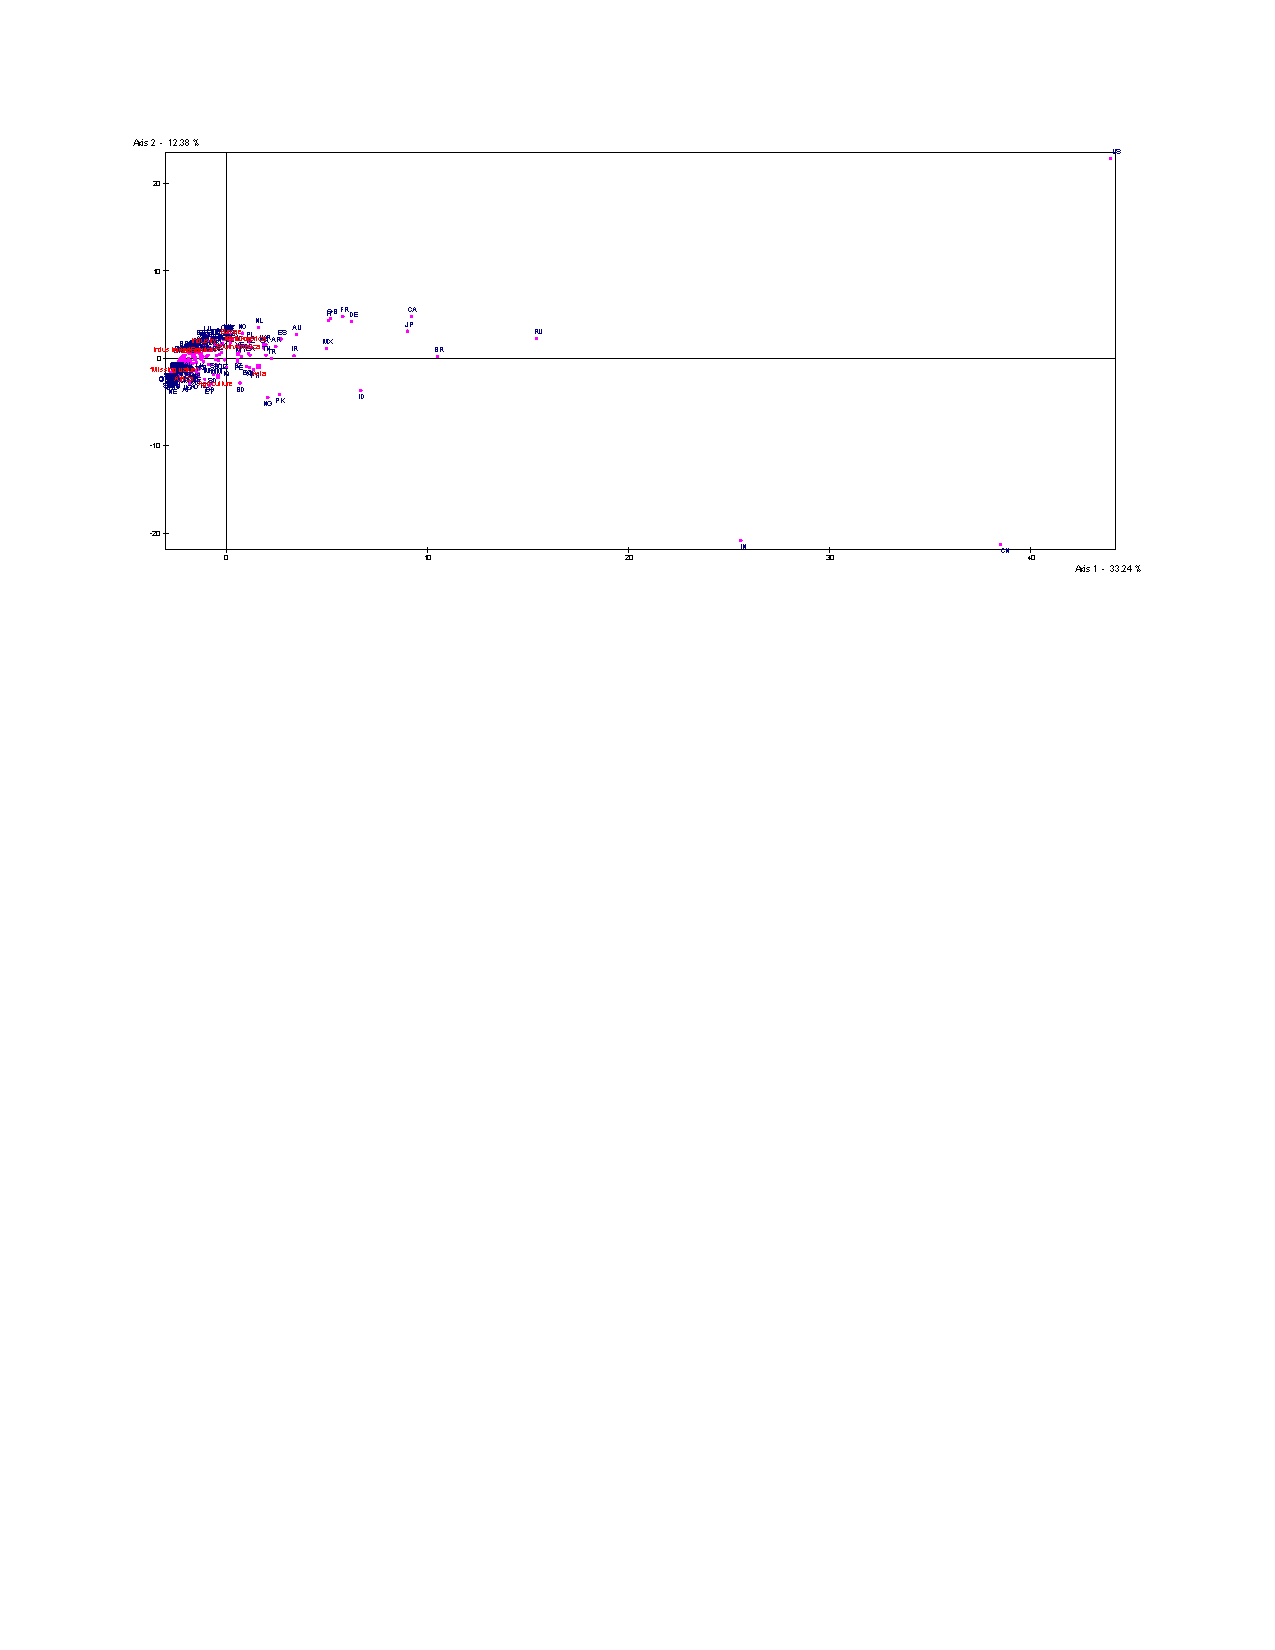
\includegraphics[width=17cm]{f2a.pdf}
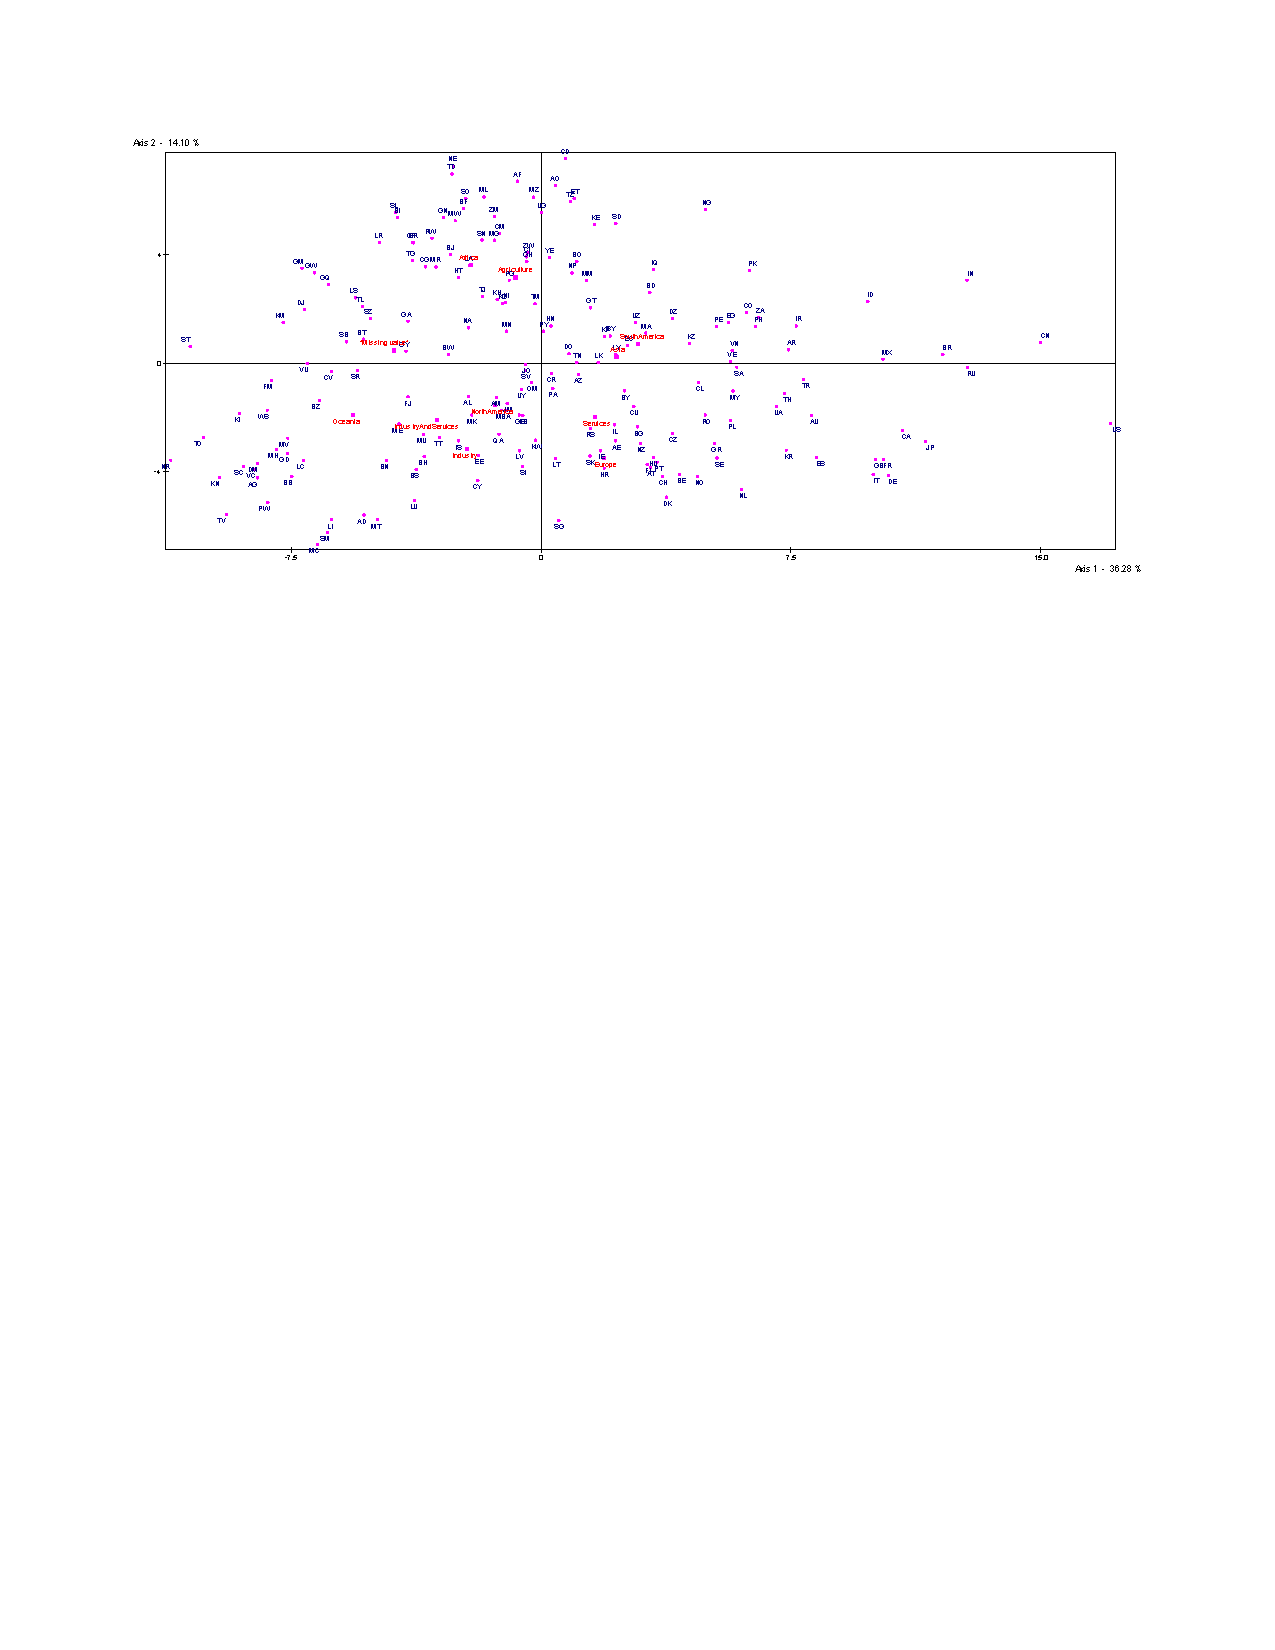
\includegraphics[width=17cm]{f2b.pdf}
\caption{\footnotesize{Comparative results of the \emph{naive} PCA using original and synthetic variables respectively. Naive PCA consists on a PCA with all continuous variables as active variables. In the PCA with the original variables, the distribution of the cloud of points is heavily left skewed, a few outliers can be seen to the right. In the PCA done with synthetic variables we see a more normal distribution of the cloud of points, thus densifiyng the center of mass still preserving roughly the order of previous observation points and the inertia of the factors.}\label{fig2}}
\end{center}
\end{figure}

\begin{figure}[!ht]
\begin{center}
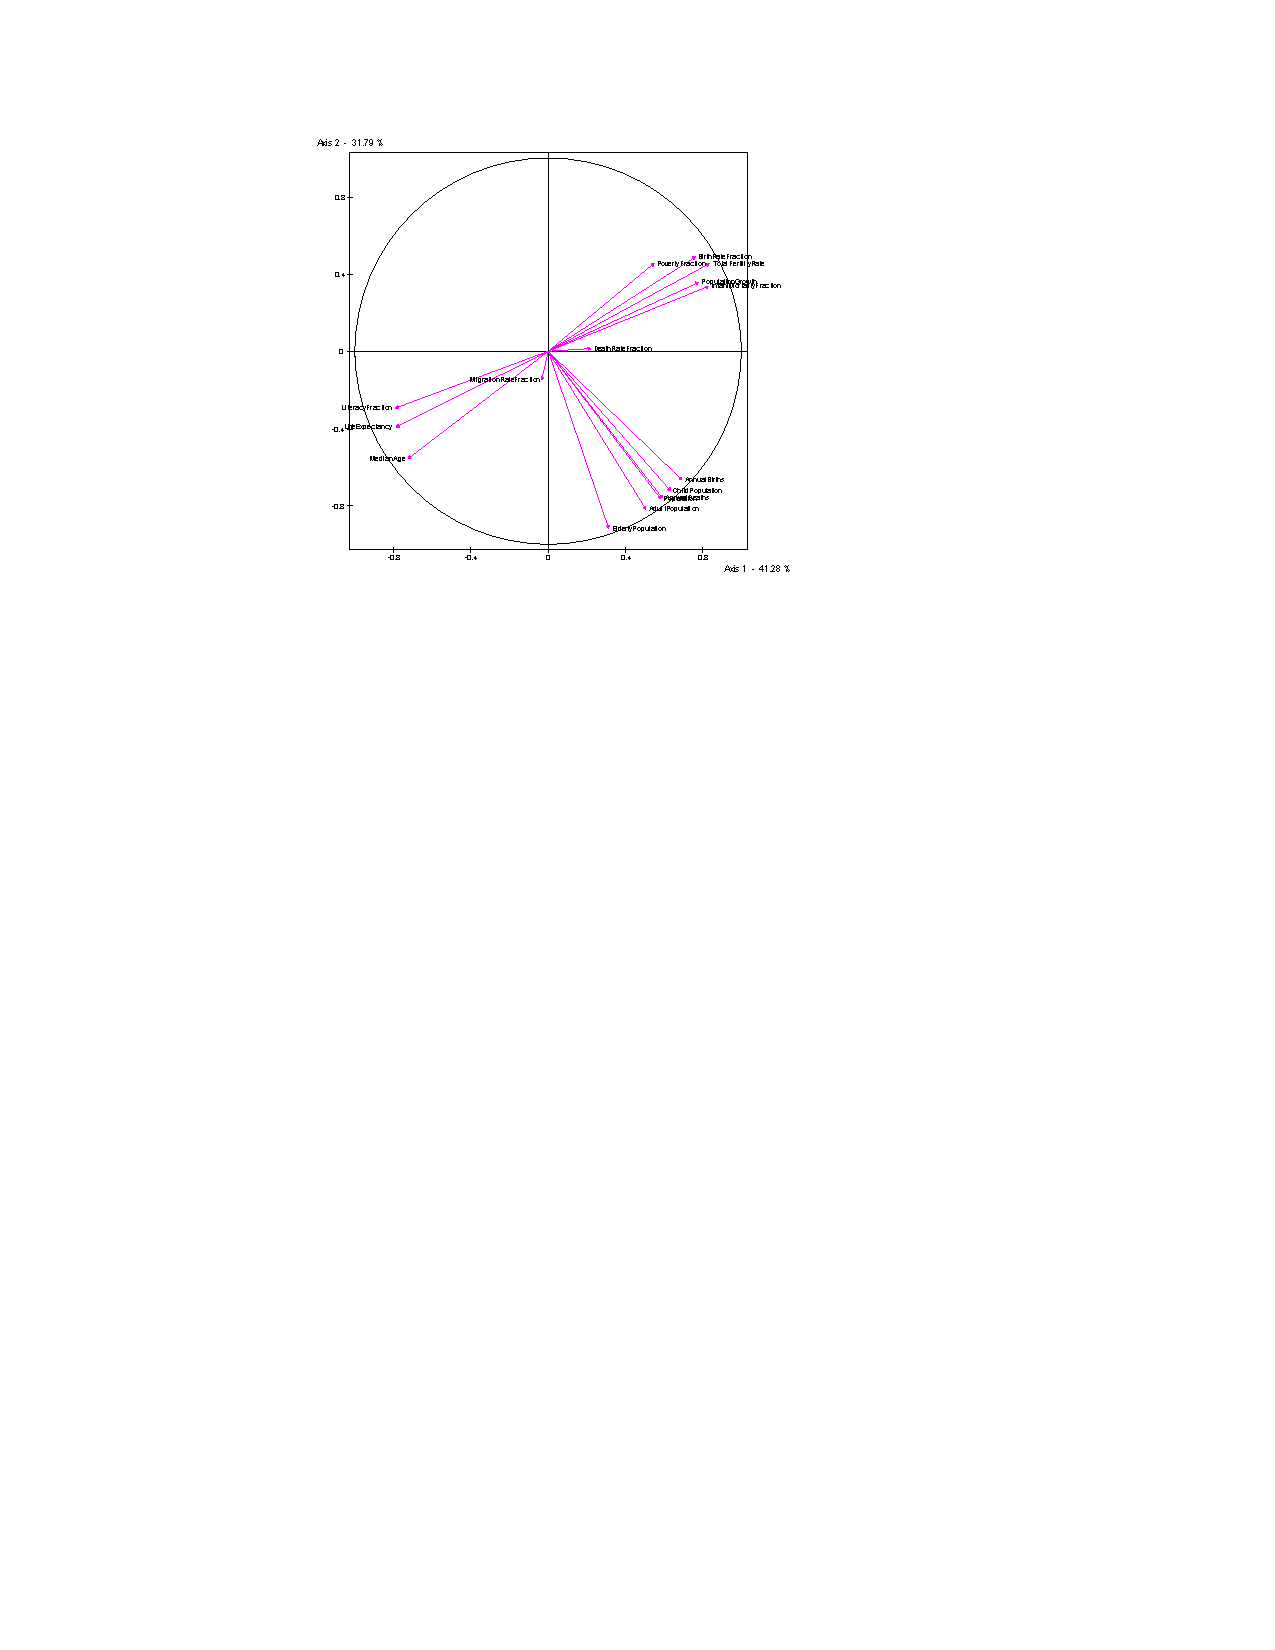
\includegraphics[width=16cm]{p1a.pdf}
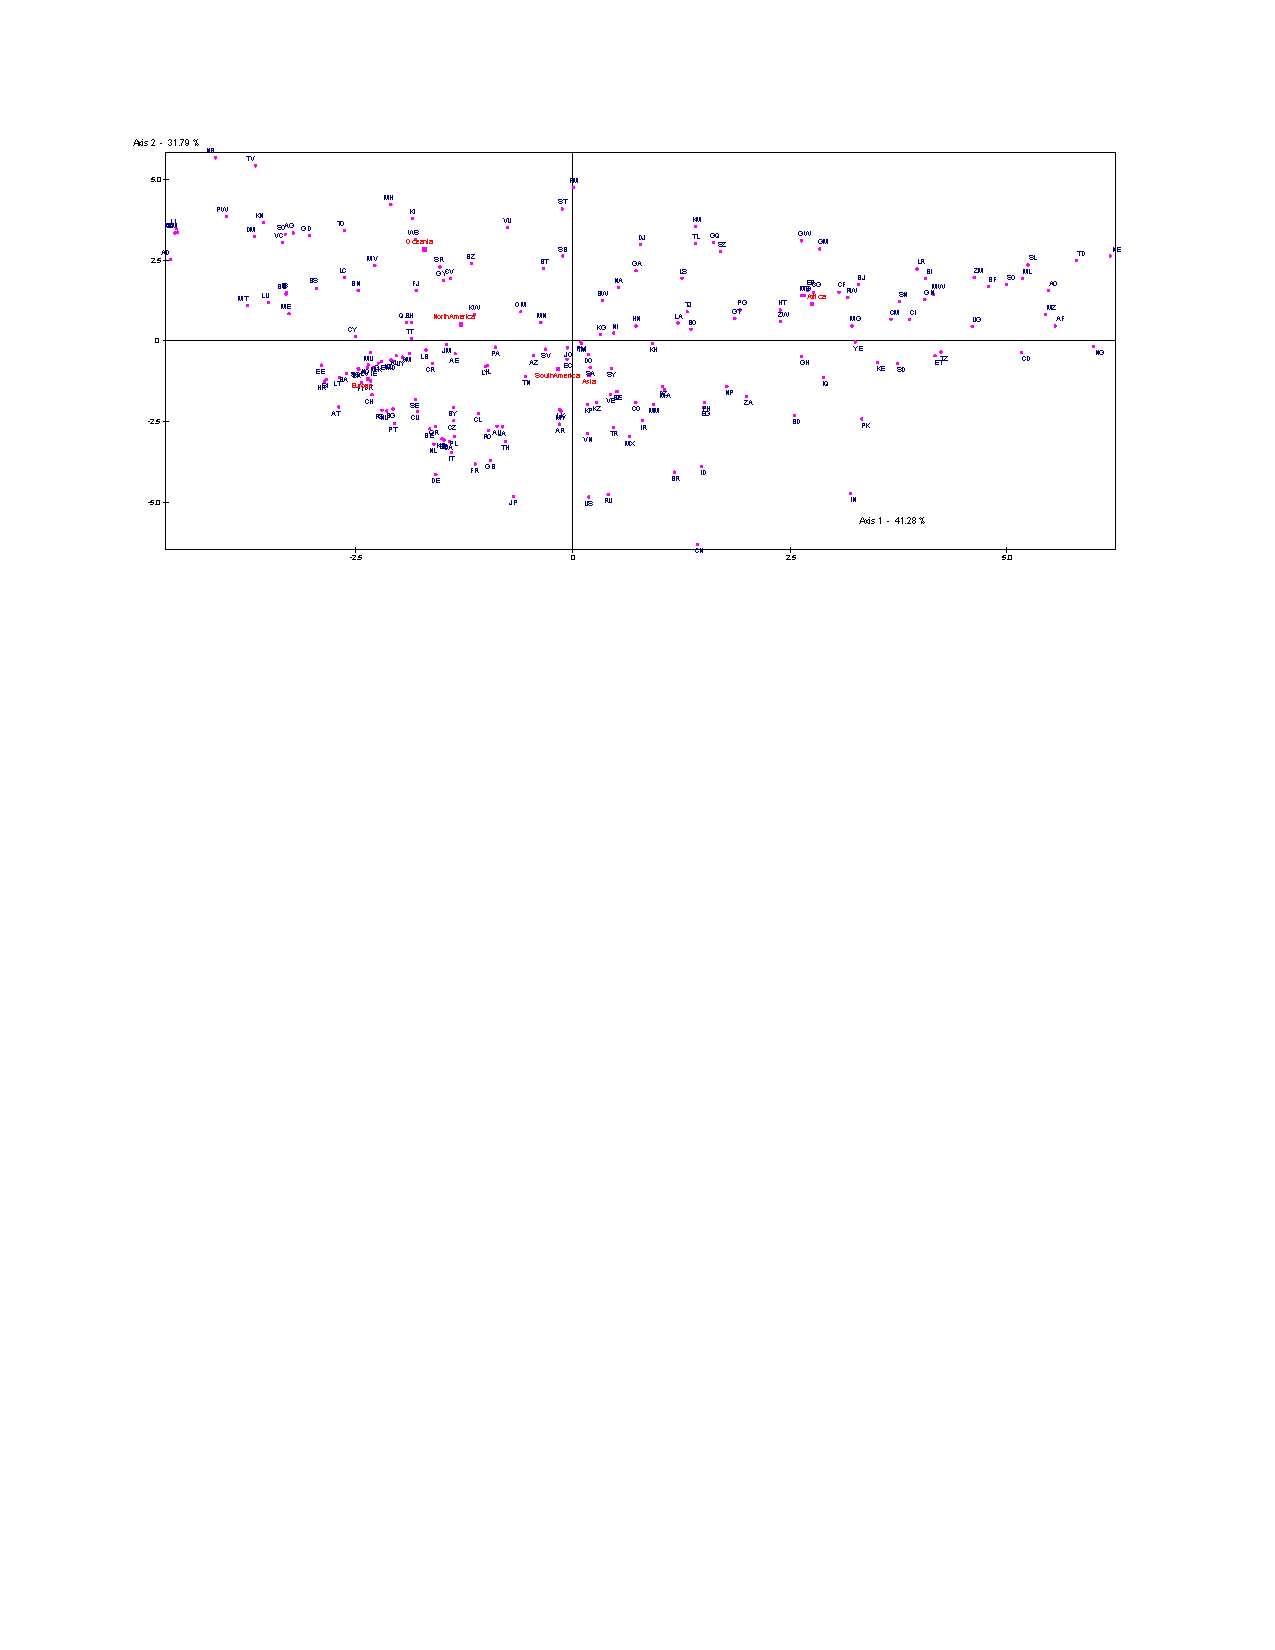
\includegraphics[width=17cm]{p1b.pdf}
\caption{\footnotesize{Results of the normed PCA carried out on the Demographic group of variables in the set.}\label{p1}}
\end{center}
\end{figure}

\begin{figure}[!ht]
\begin{center}
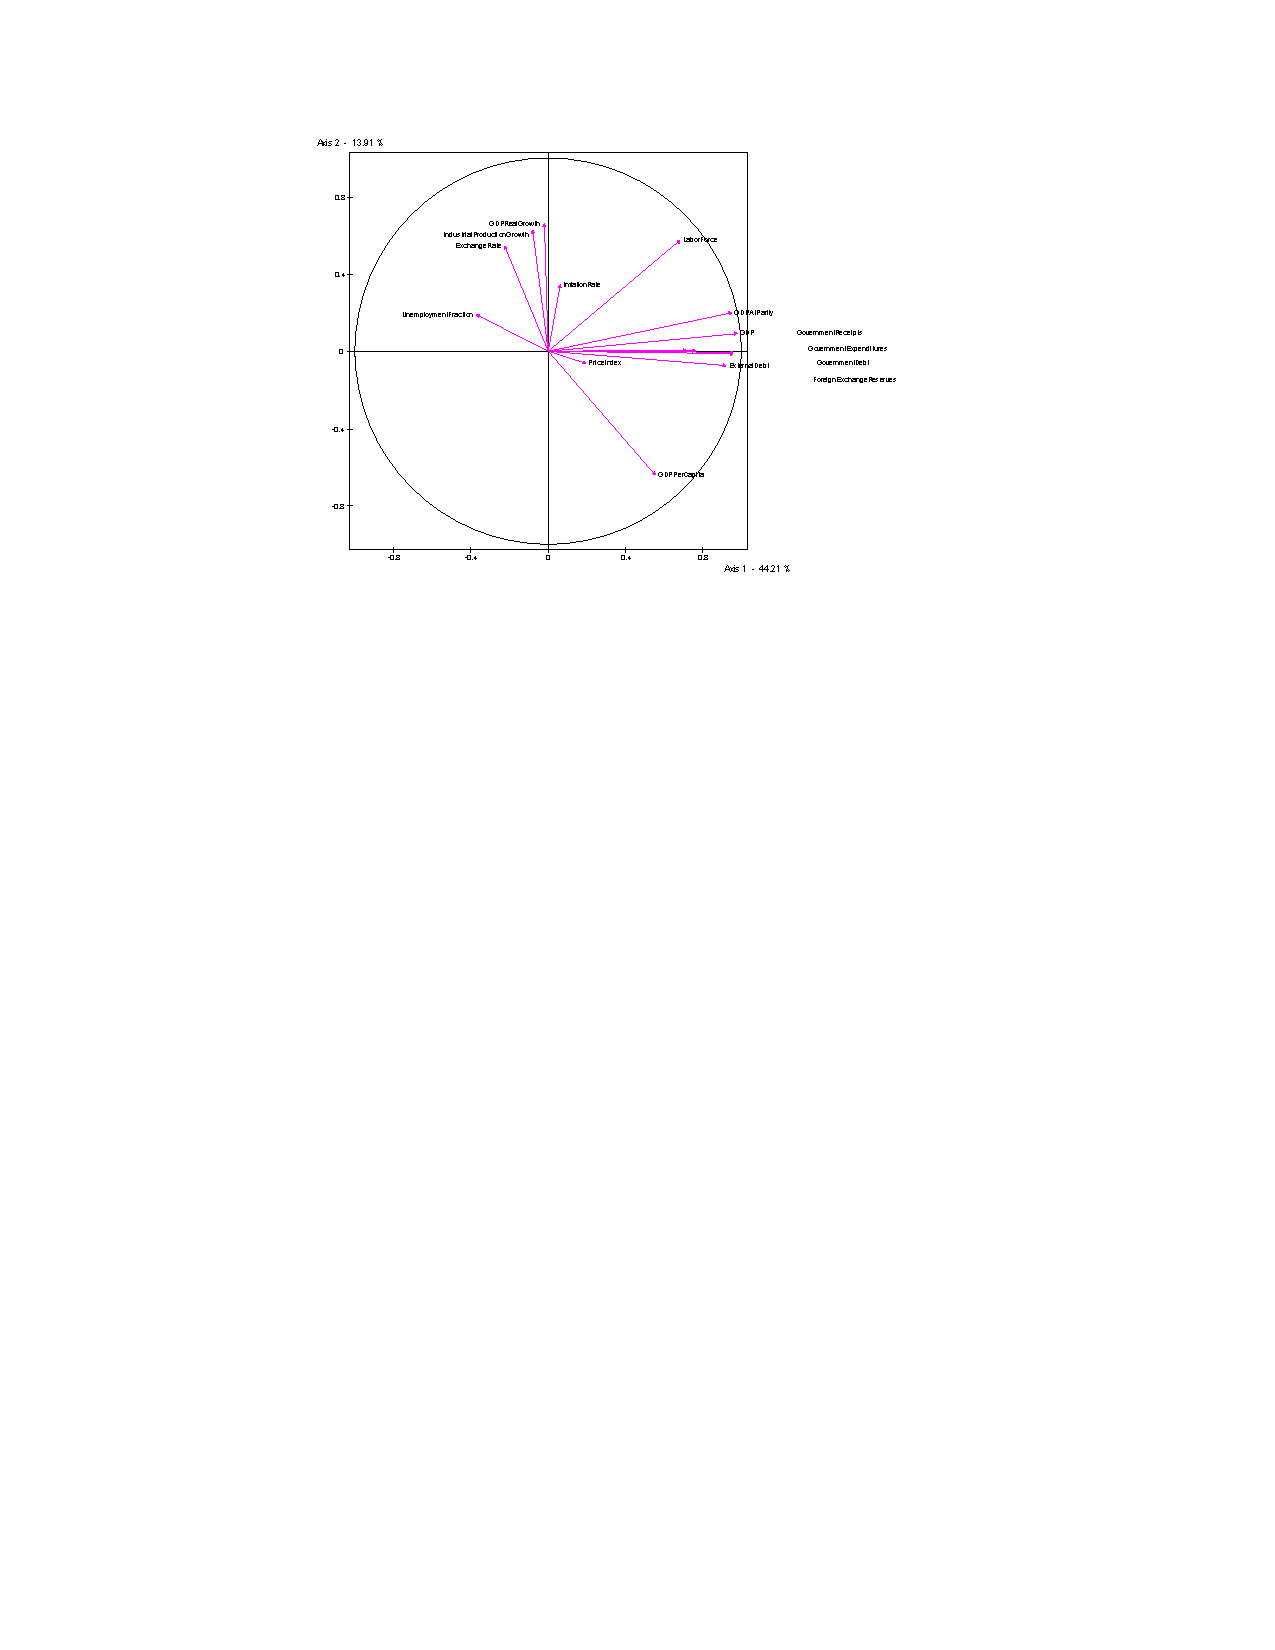
\includegraphics[width=16cm]{p2a.pdf}
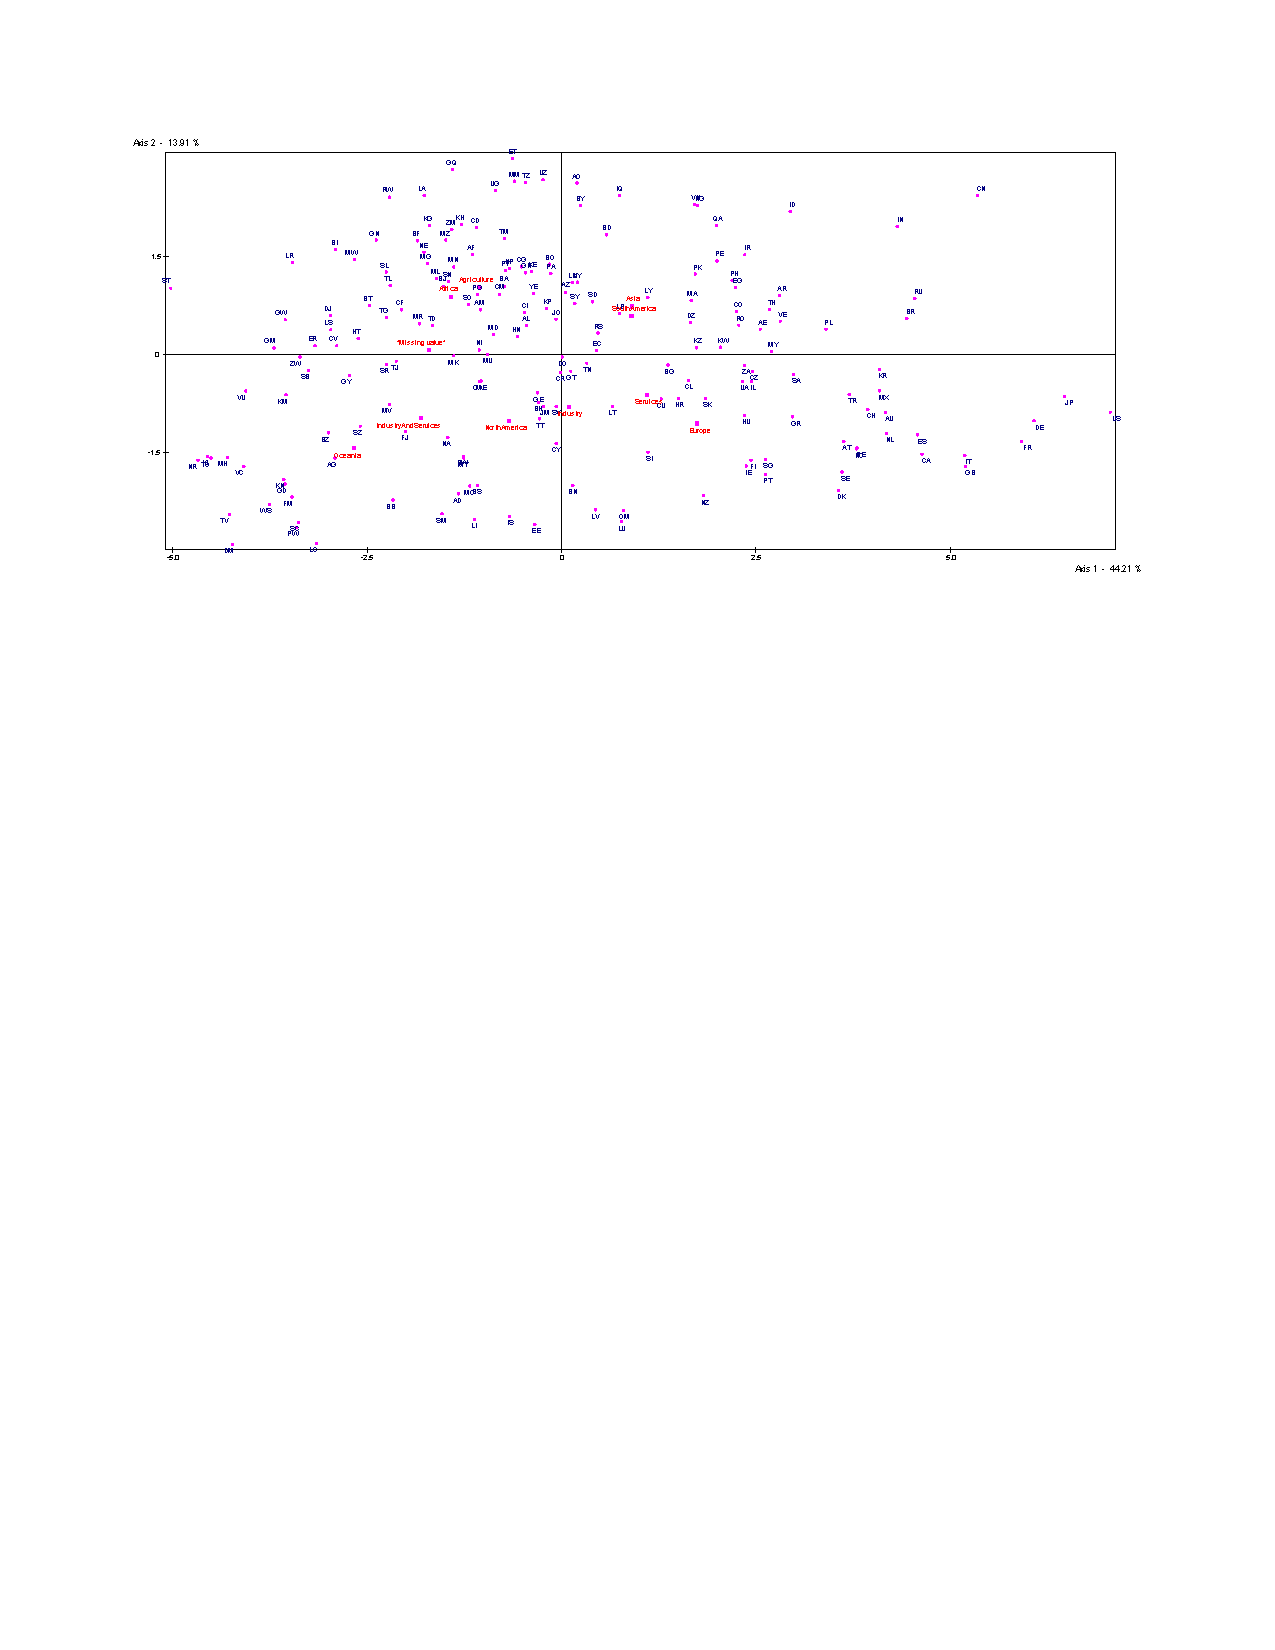
\includegraphics[width=17cm]{p2b.pdf}
\caption{\footnotesize{Results of the normed PCA carried out on the Economic group of variables in the set.}\label{p2}}
\end{center}
\end{figure}

\begin{figure}[!ht]
\begin{center}
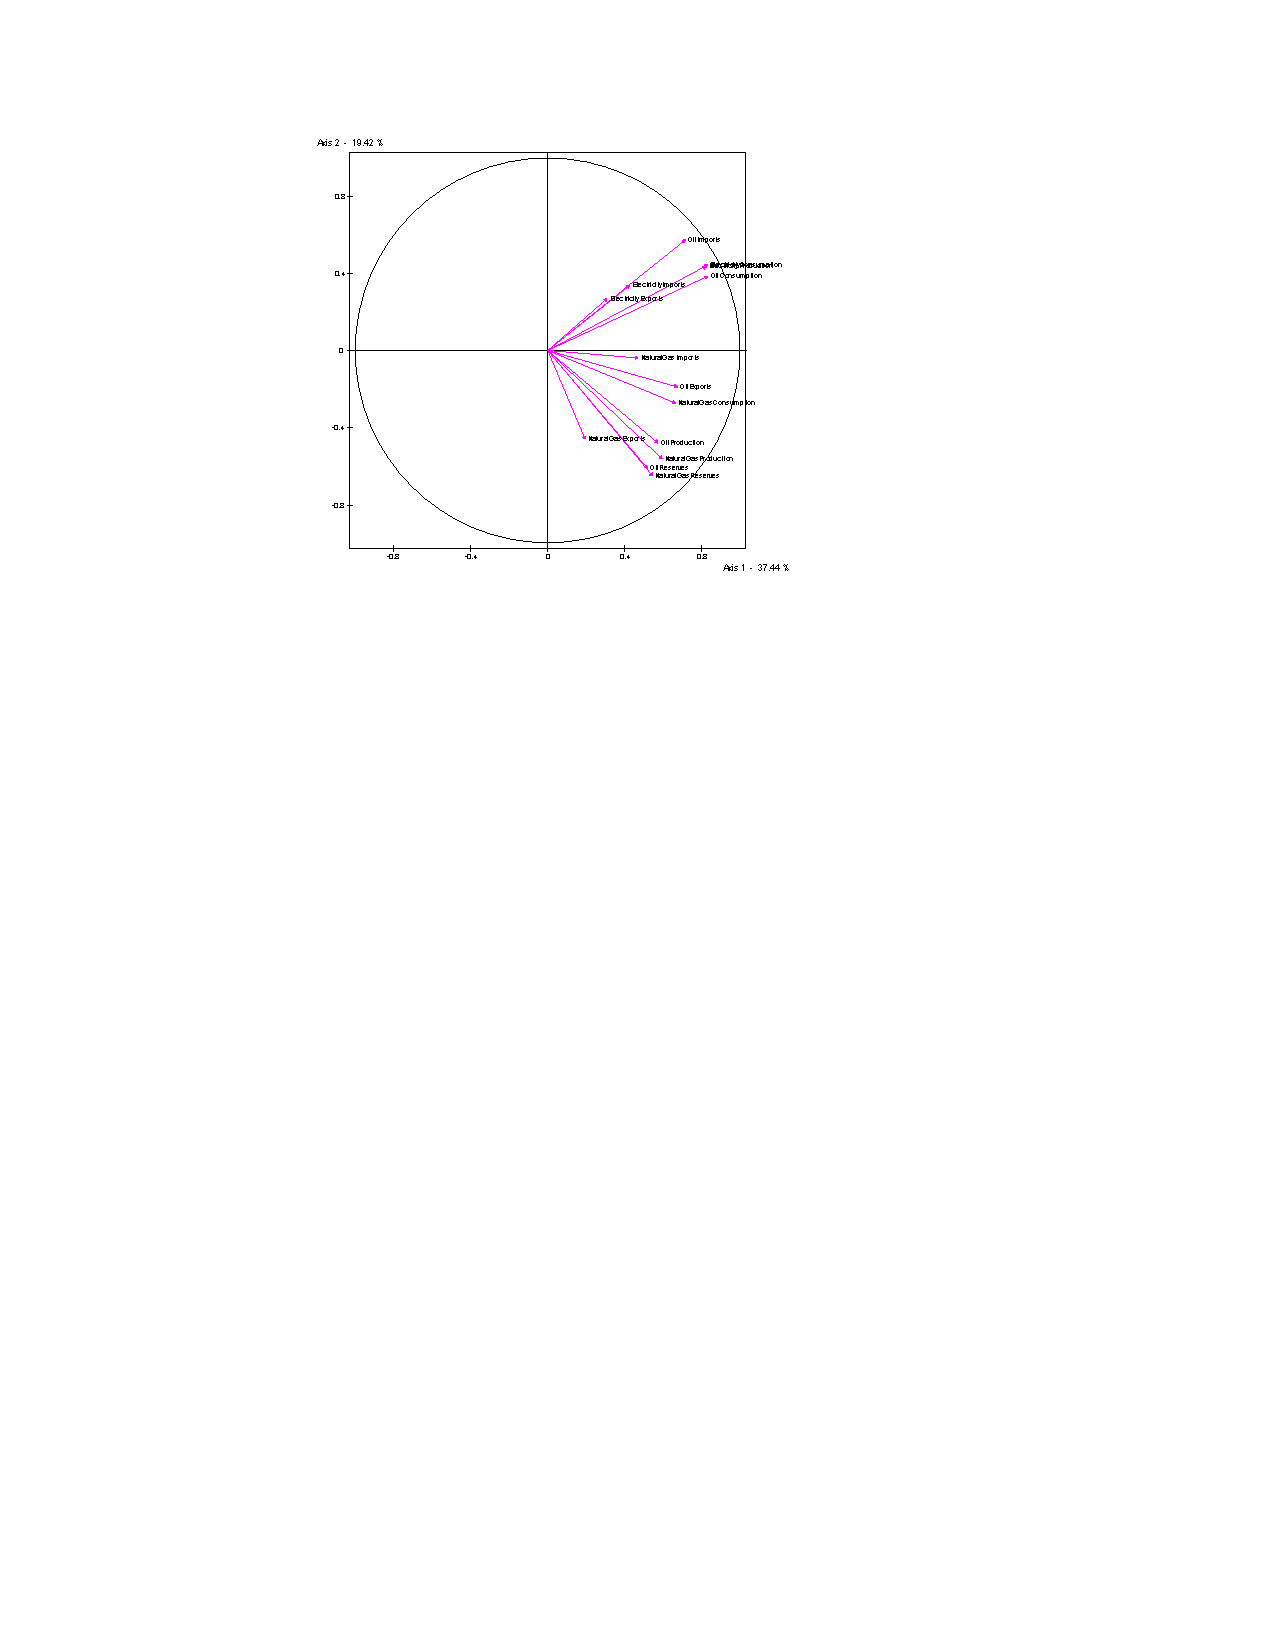
\includegraphics[width=16cm]{p3a.pdf}
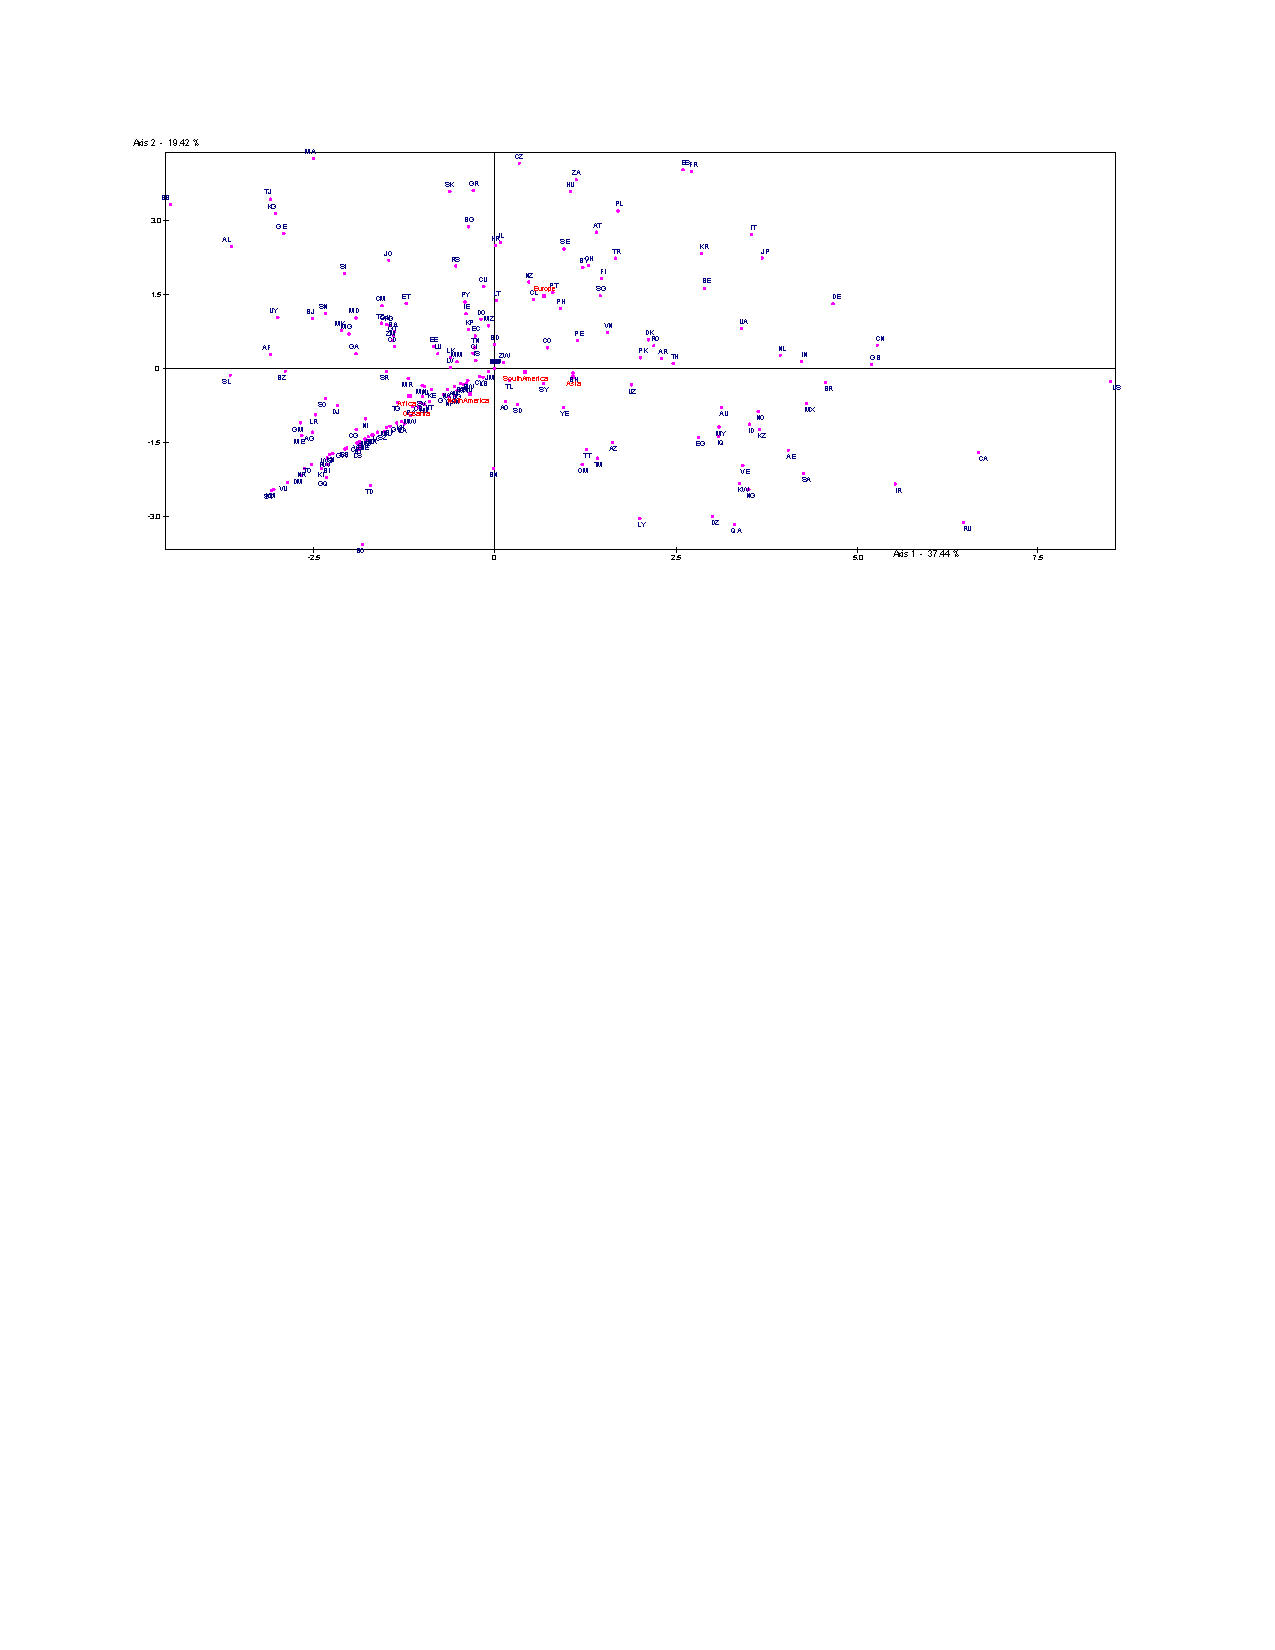
\includegraphics[width=17cm]{p3b.pdf}
\caption{\footnotesize{Results of the normed PCA carried out on the Energy group of variables in the set.}\label{p3}}
\end{center}
\end{figure}

\begin{figure}[!ht]
\begin{center}
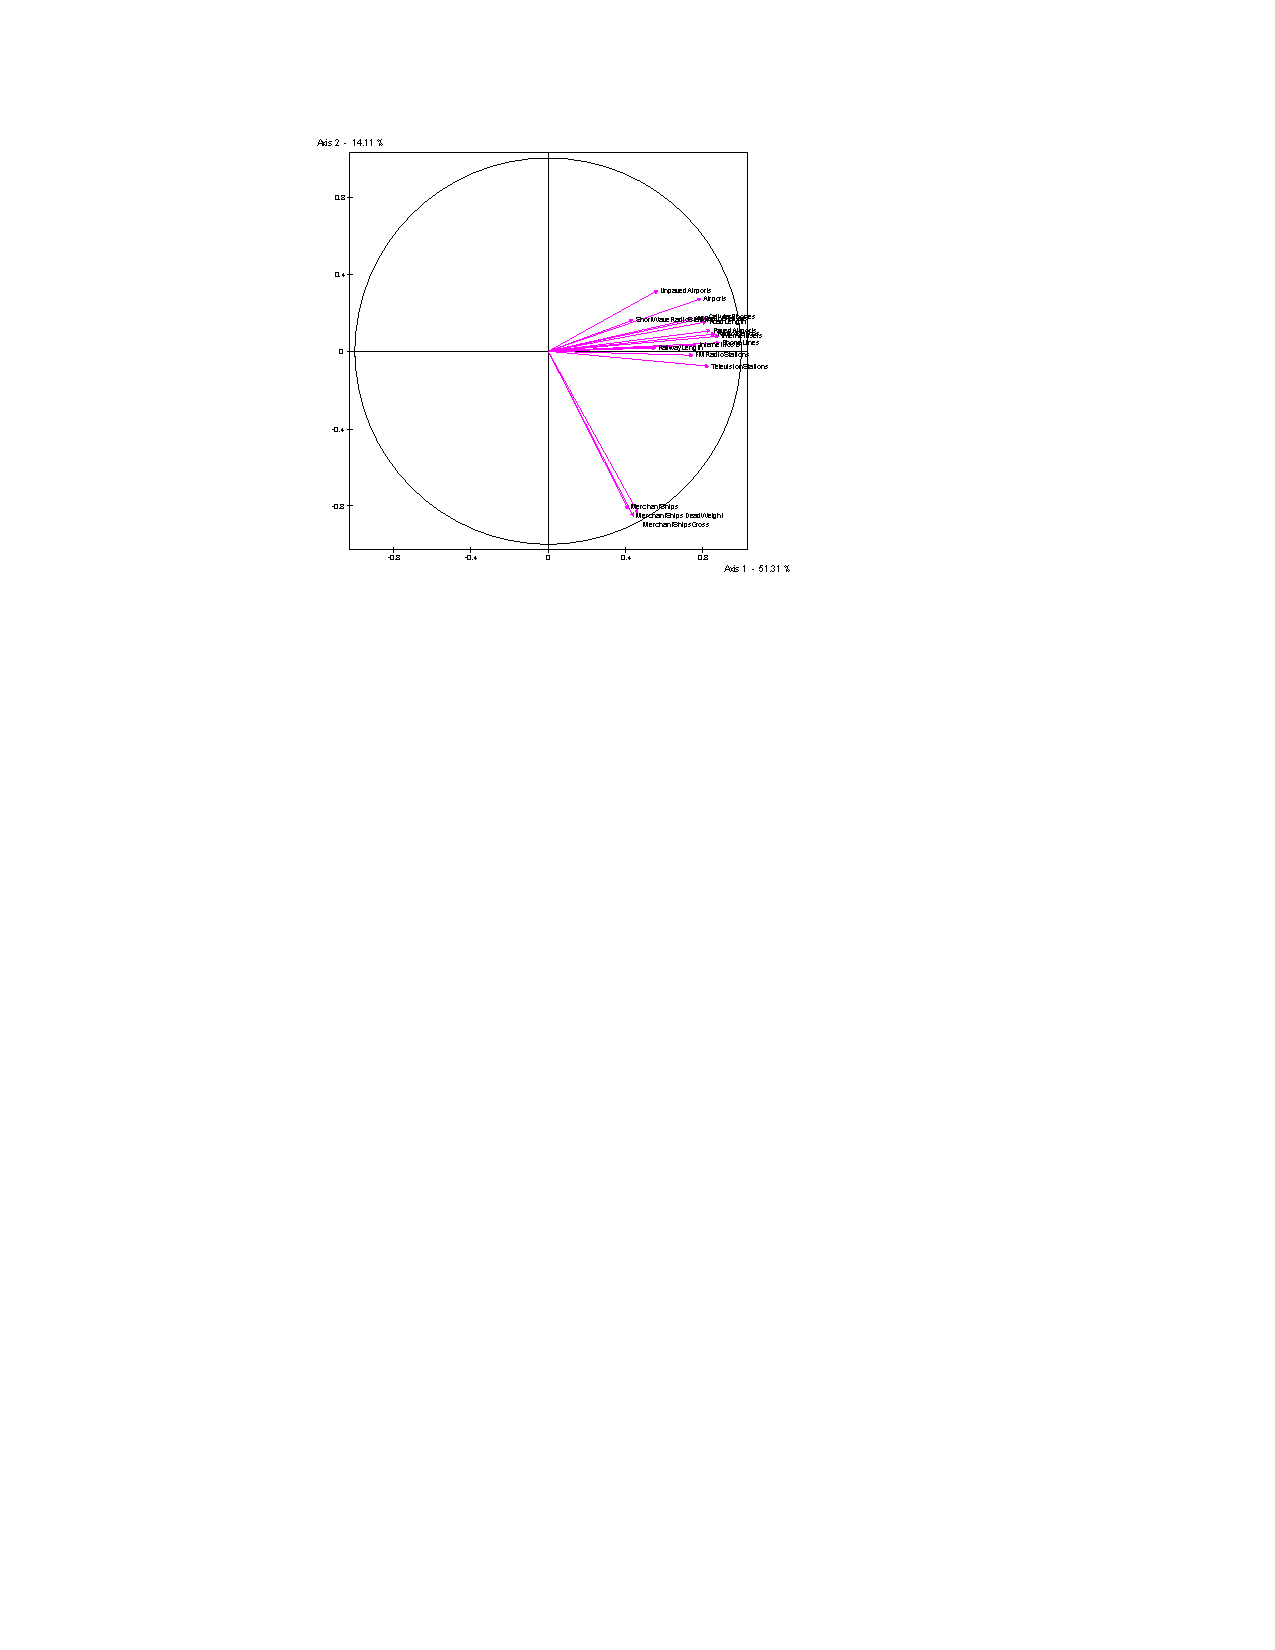
\includegraphics[width=16cm]{p4a.pdf}
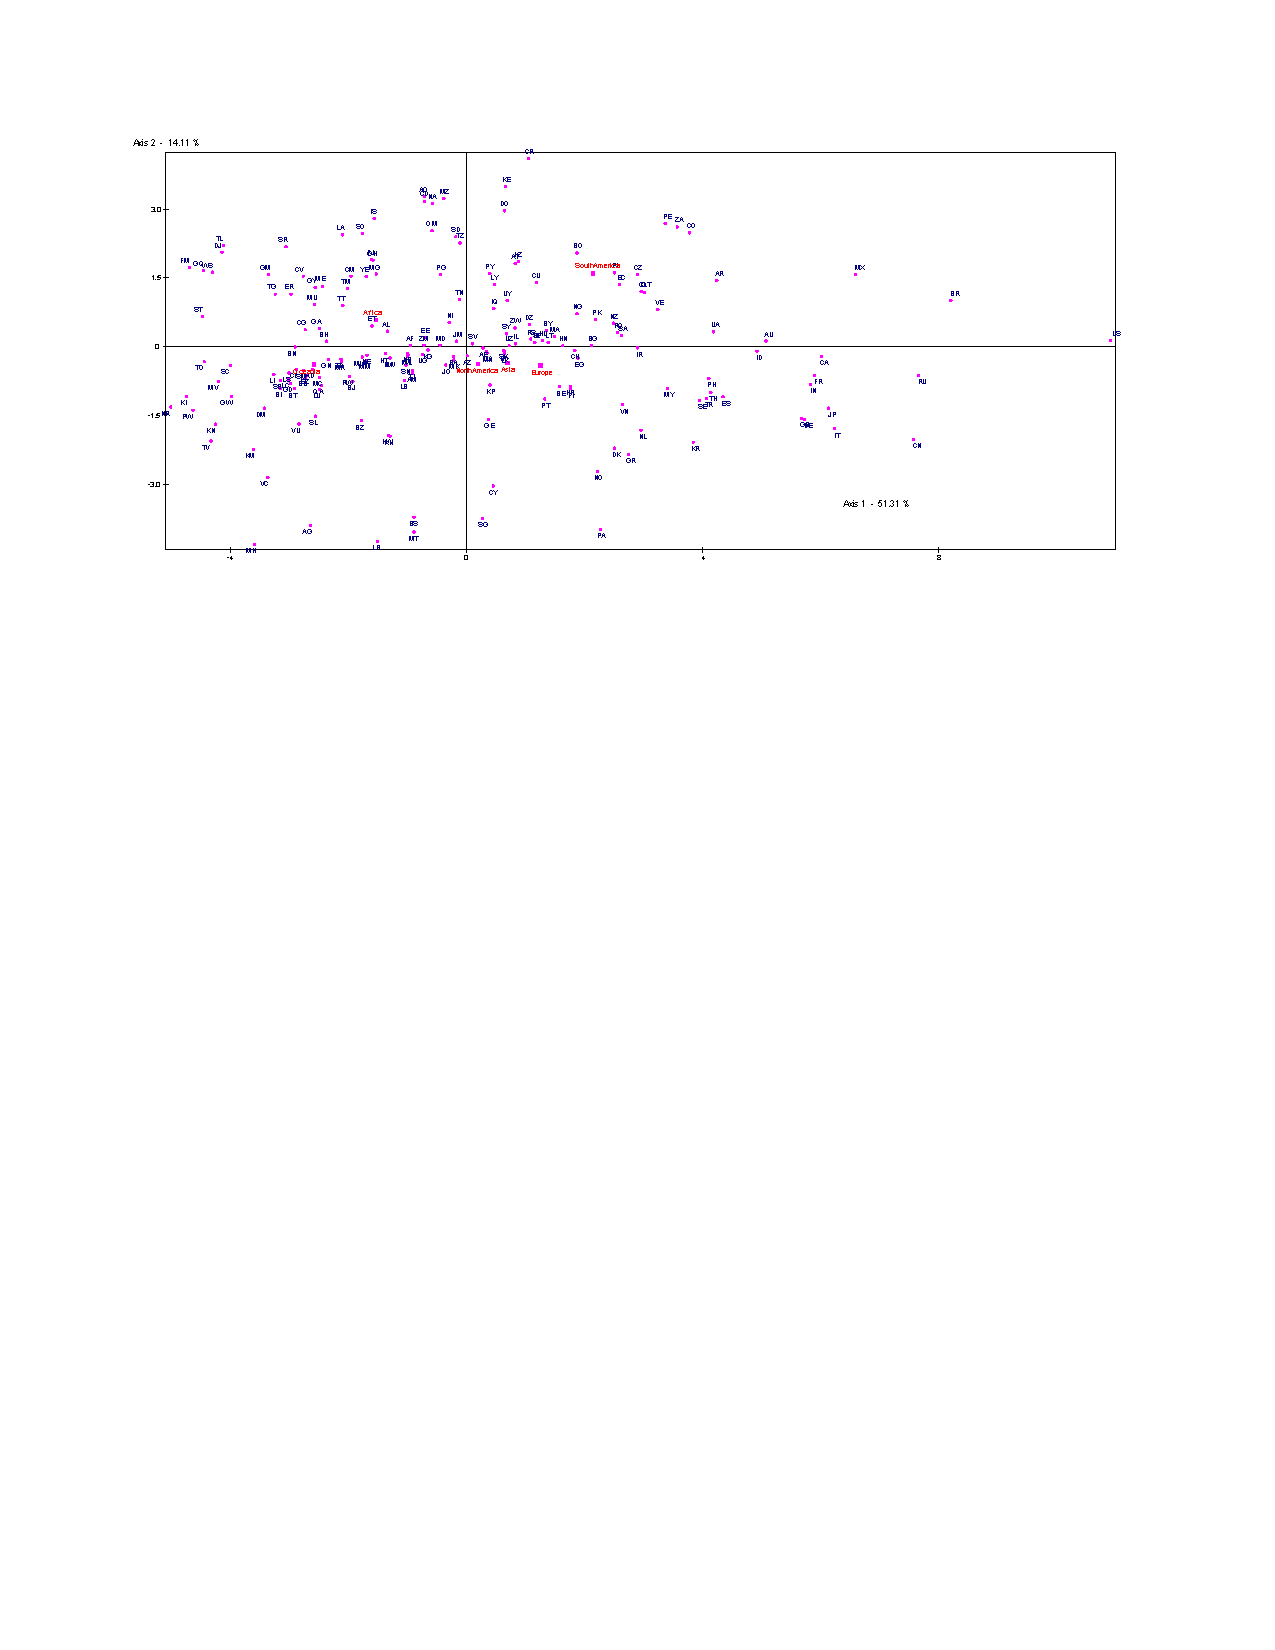
\includegraphics[width=17cm]{p4b.pdf}
\caption{\footnotesize{Results of the normed PCA carried out on the Communication group of variables in the set.}\label{p4}}
\end{center}
\end{figure}

\begin{figure}[!ht]
\begin{center}
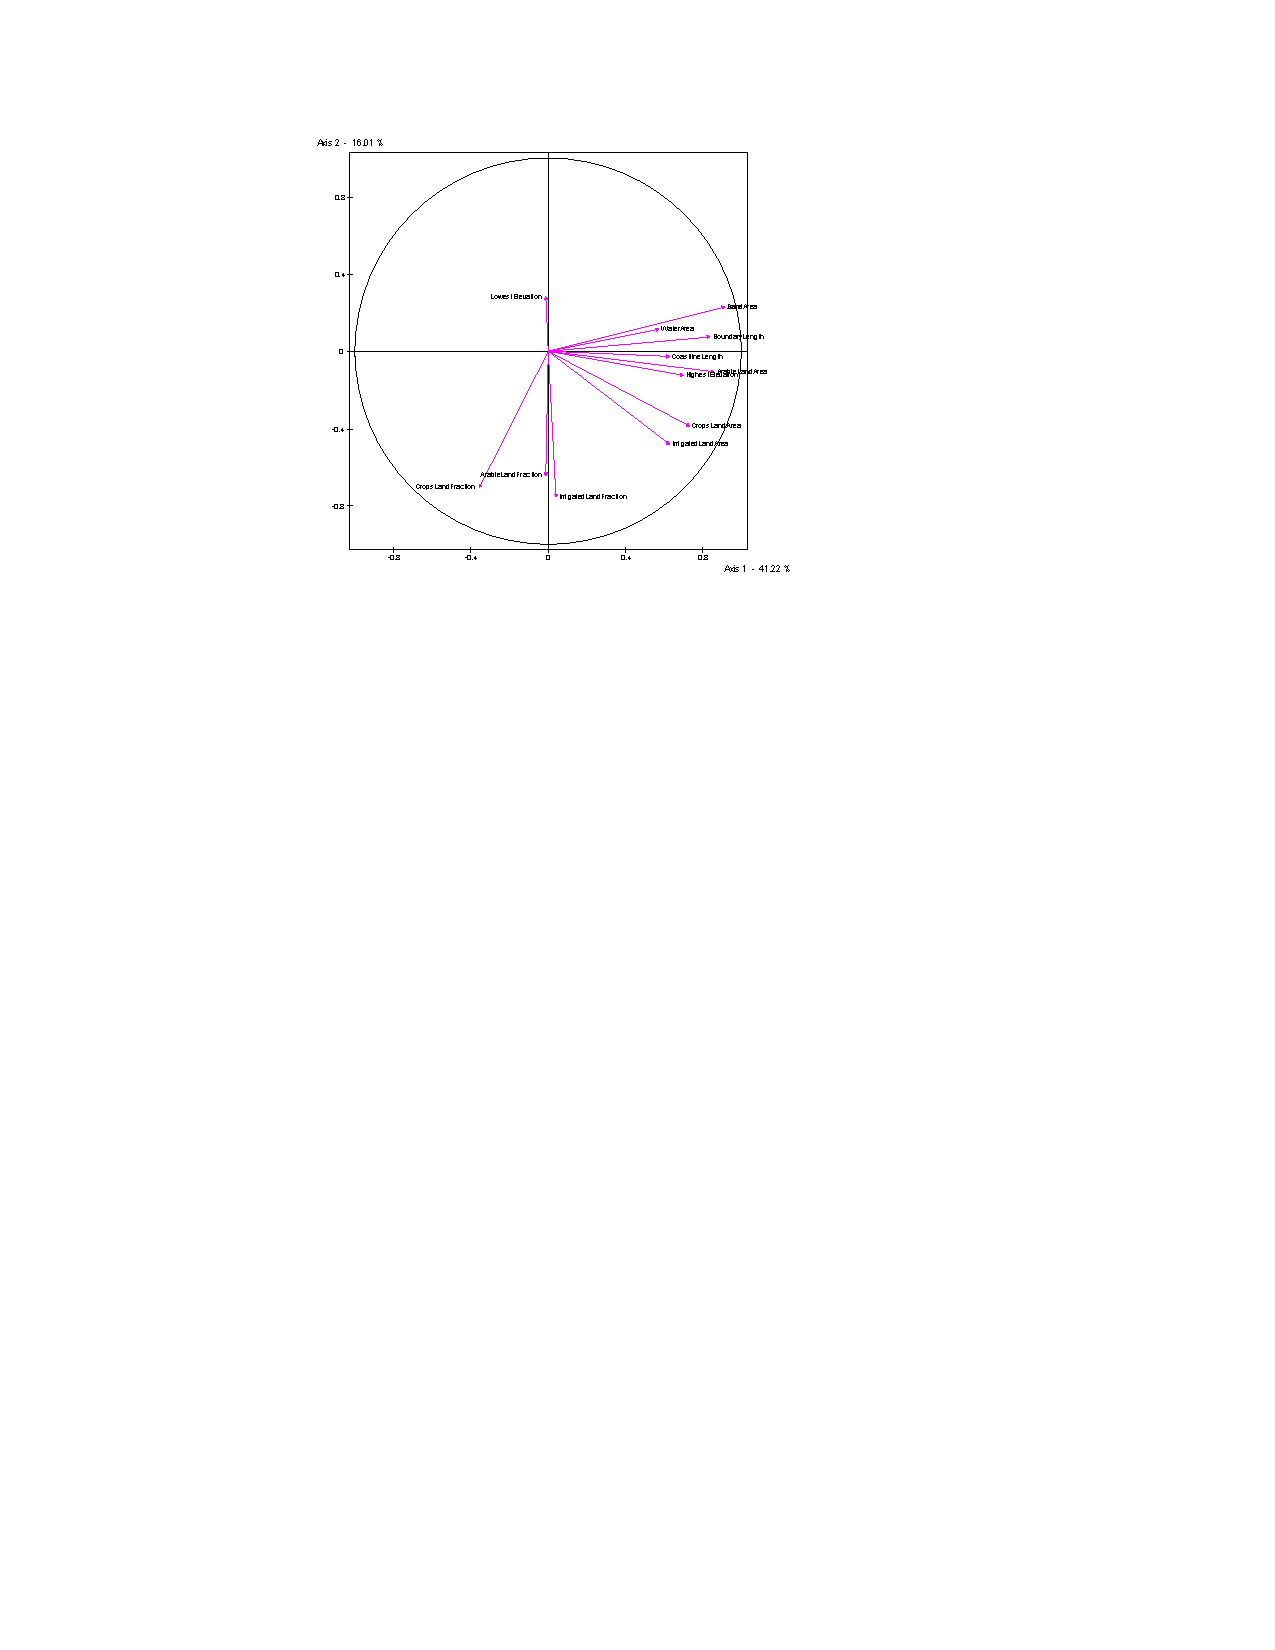
\includegraphics[width=16cm]{p5a.pdf}
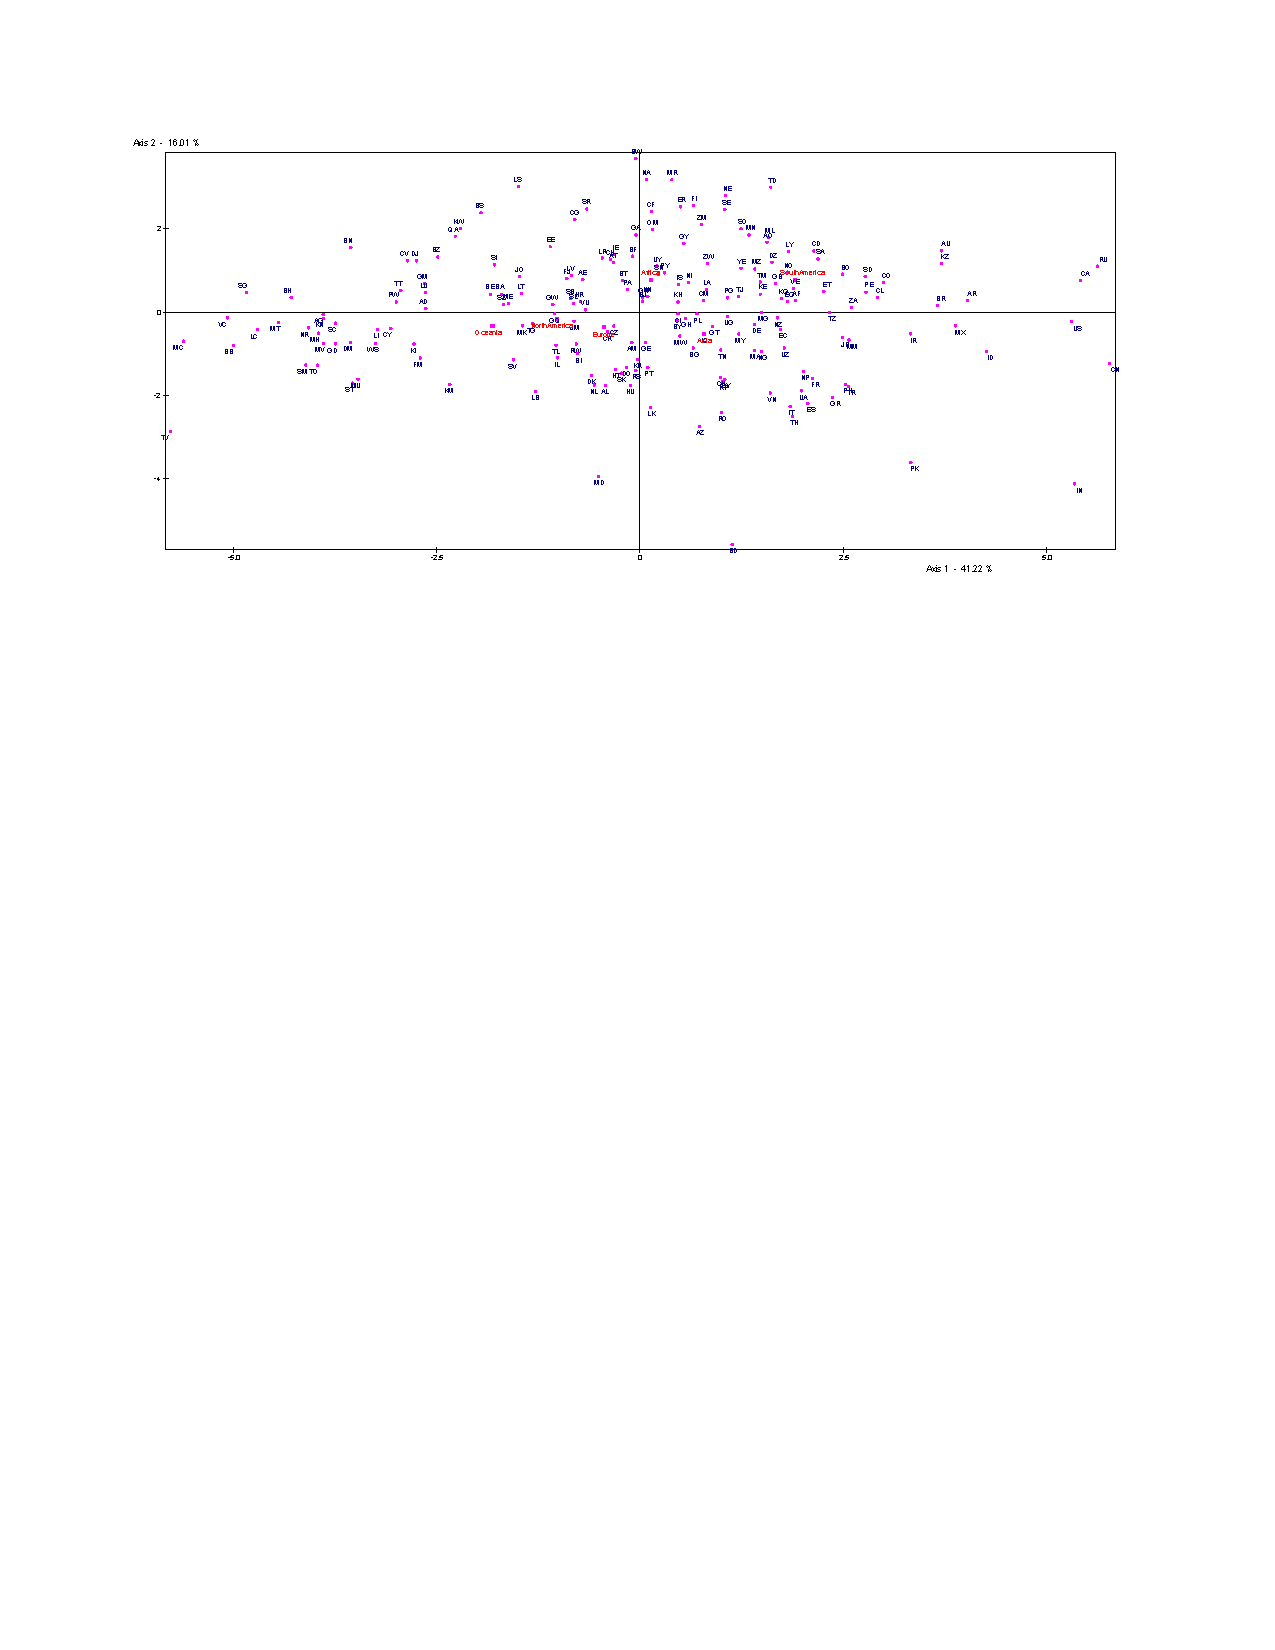
\includegraphics[width=17cm]{p5b.pdf}
\caption{\footnotesize{Results of the normed PCA carried out on the Geography group of variables in the set.}\label{p5}}
\end{center}
\end{figure}

\begin{figure}[!ht]
\begin{center}
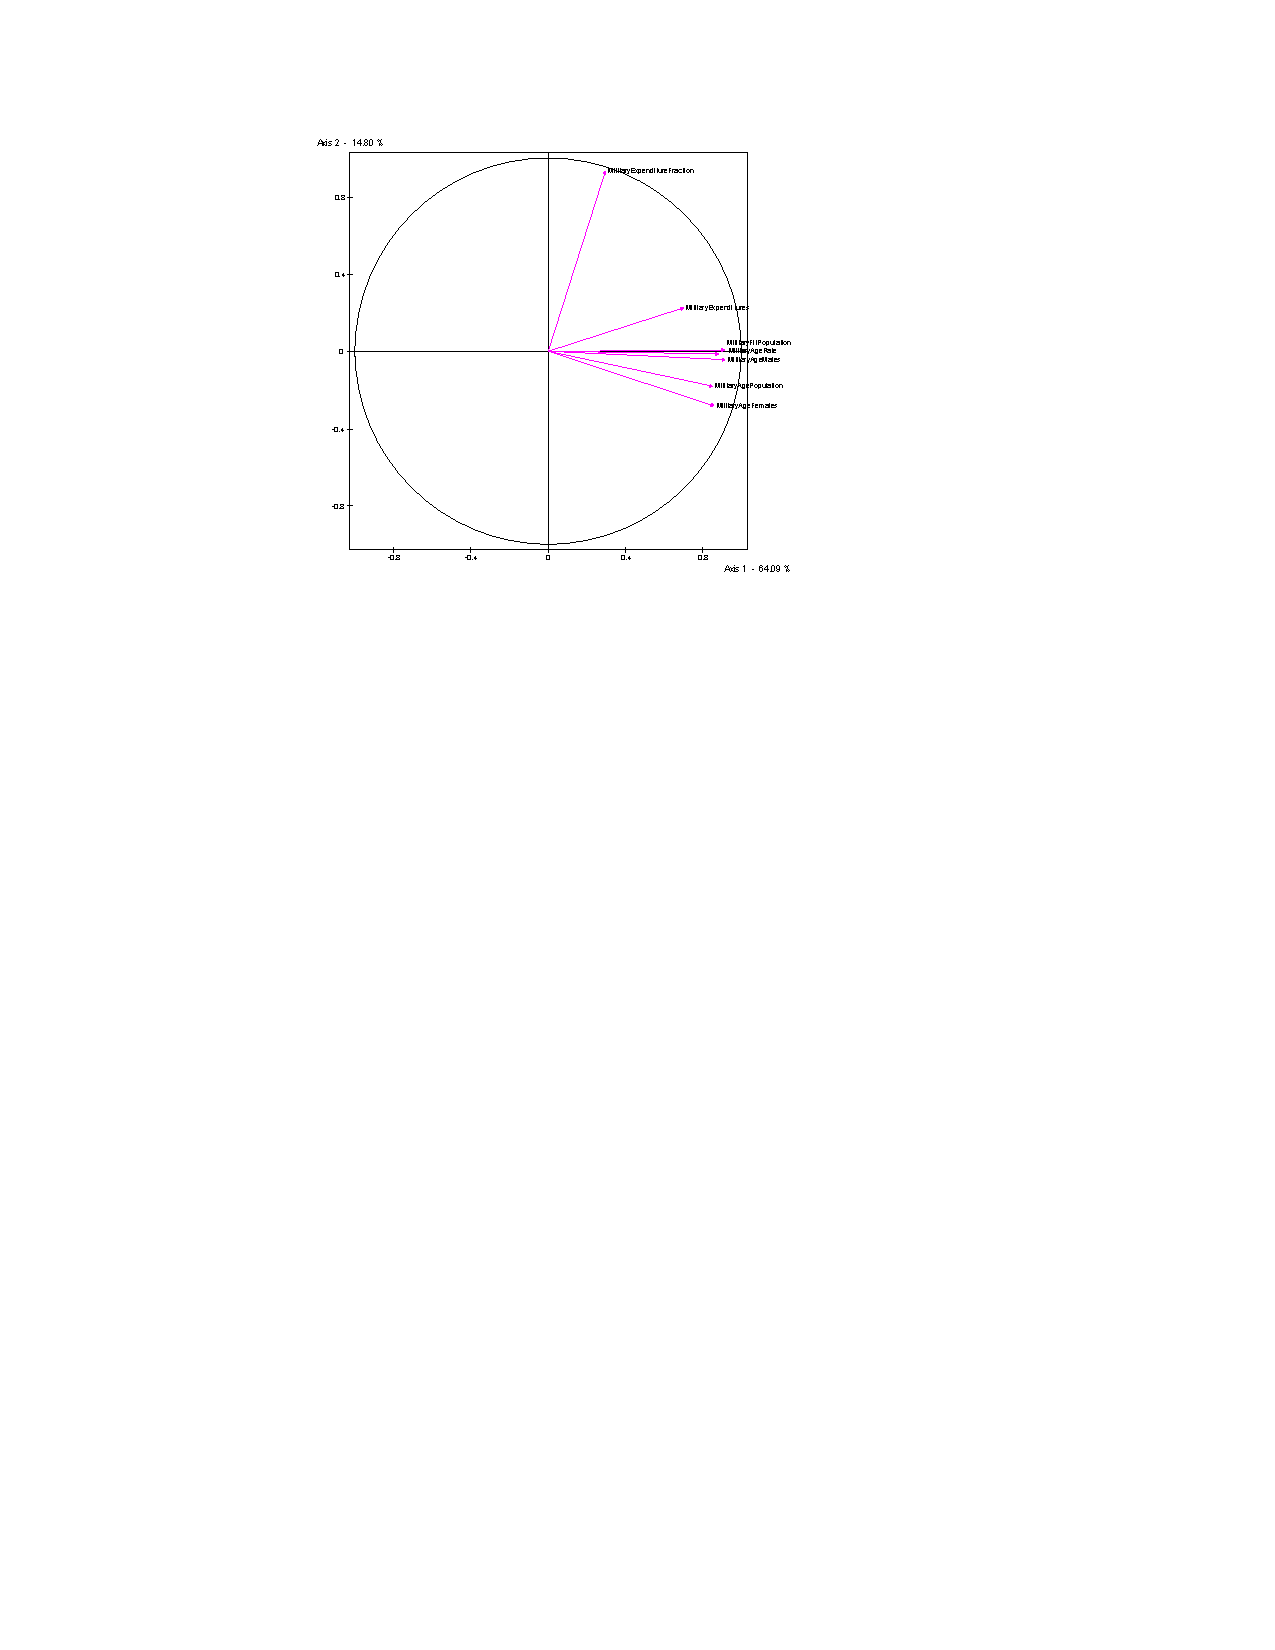
\includegraphics[width=16cm]{p6a.pdf}
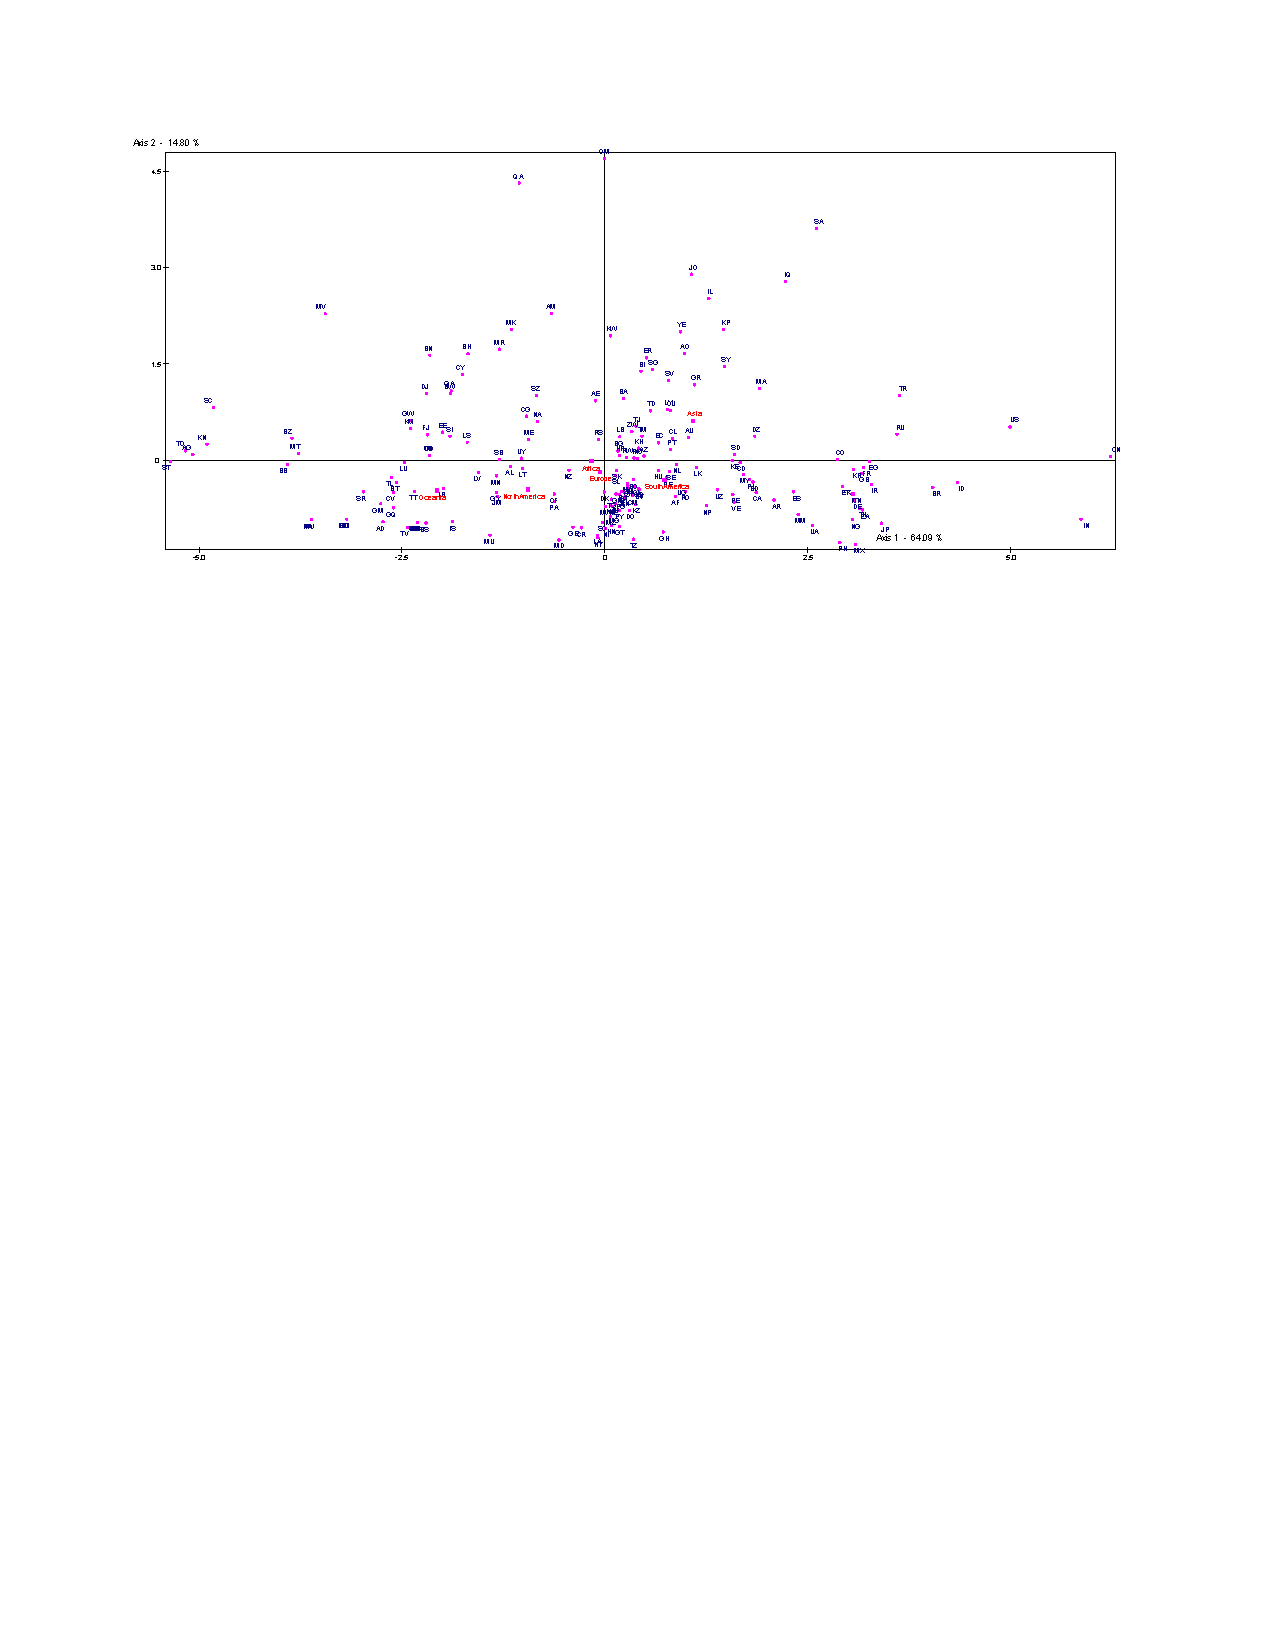
\includegraphics[width=17cm]{p6b.pdf}
\caption{\footnotesize{Results of the normed PCA carried out on the Military group of variables in the set.}\label{p6}}
\end{center}
\end{figure}


\begin{figure}[!ht]
\begin{center}
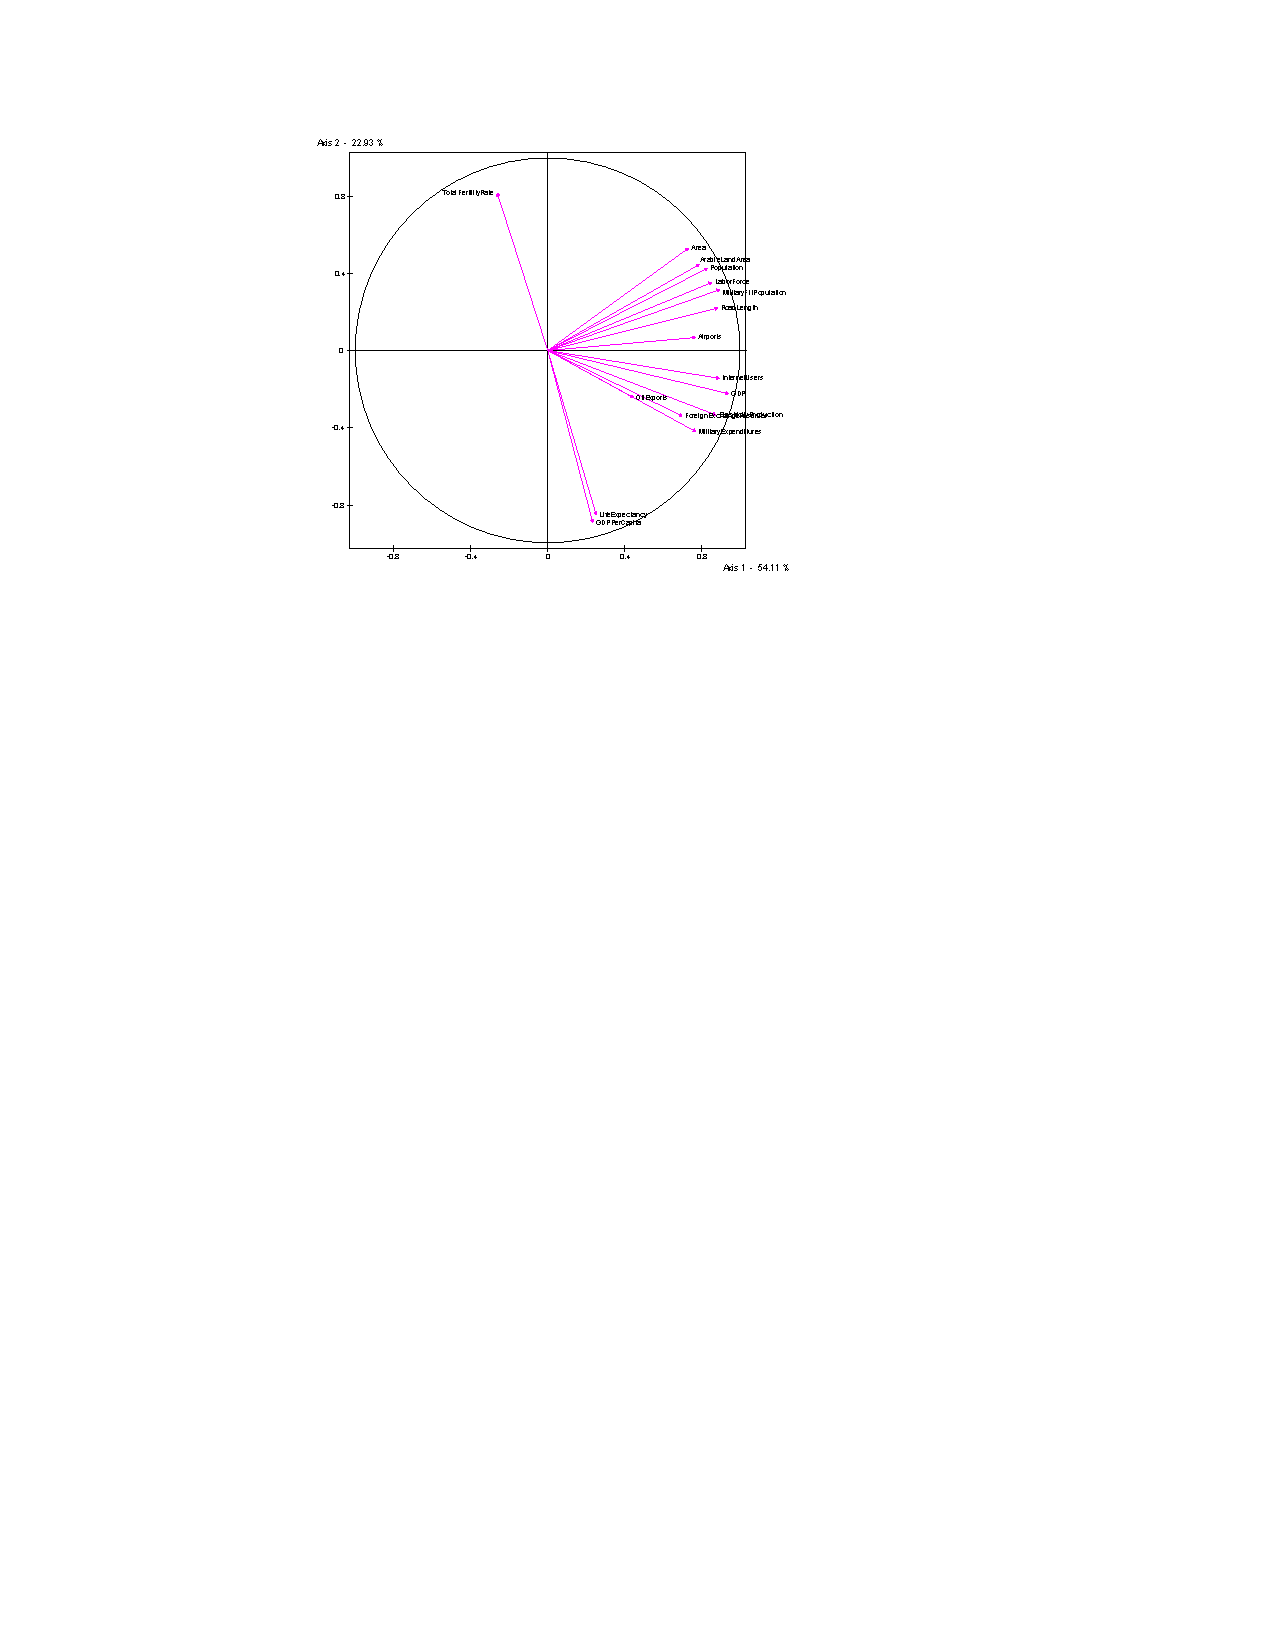
\includegraphics[width=16cm]{r2.pdf}
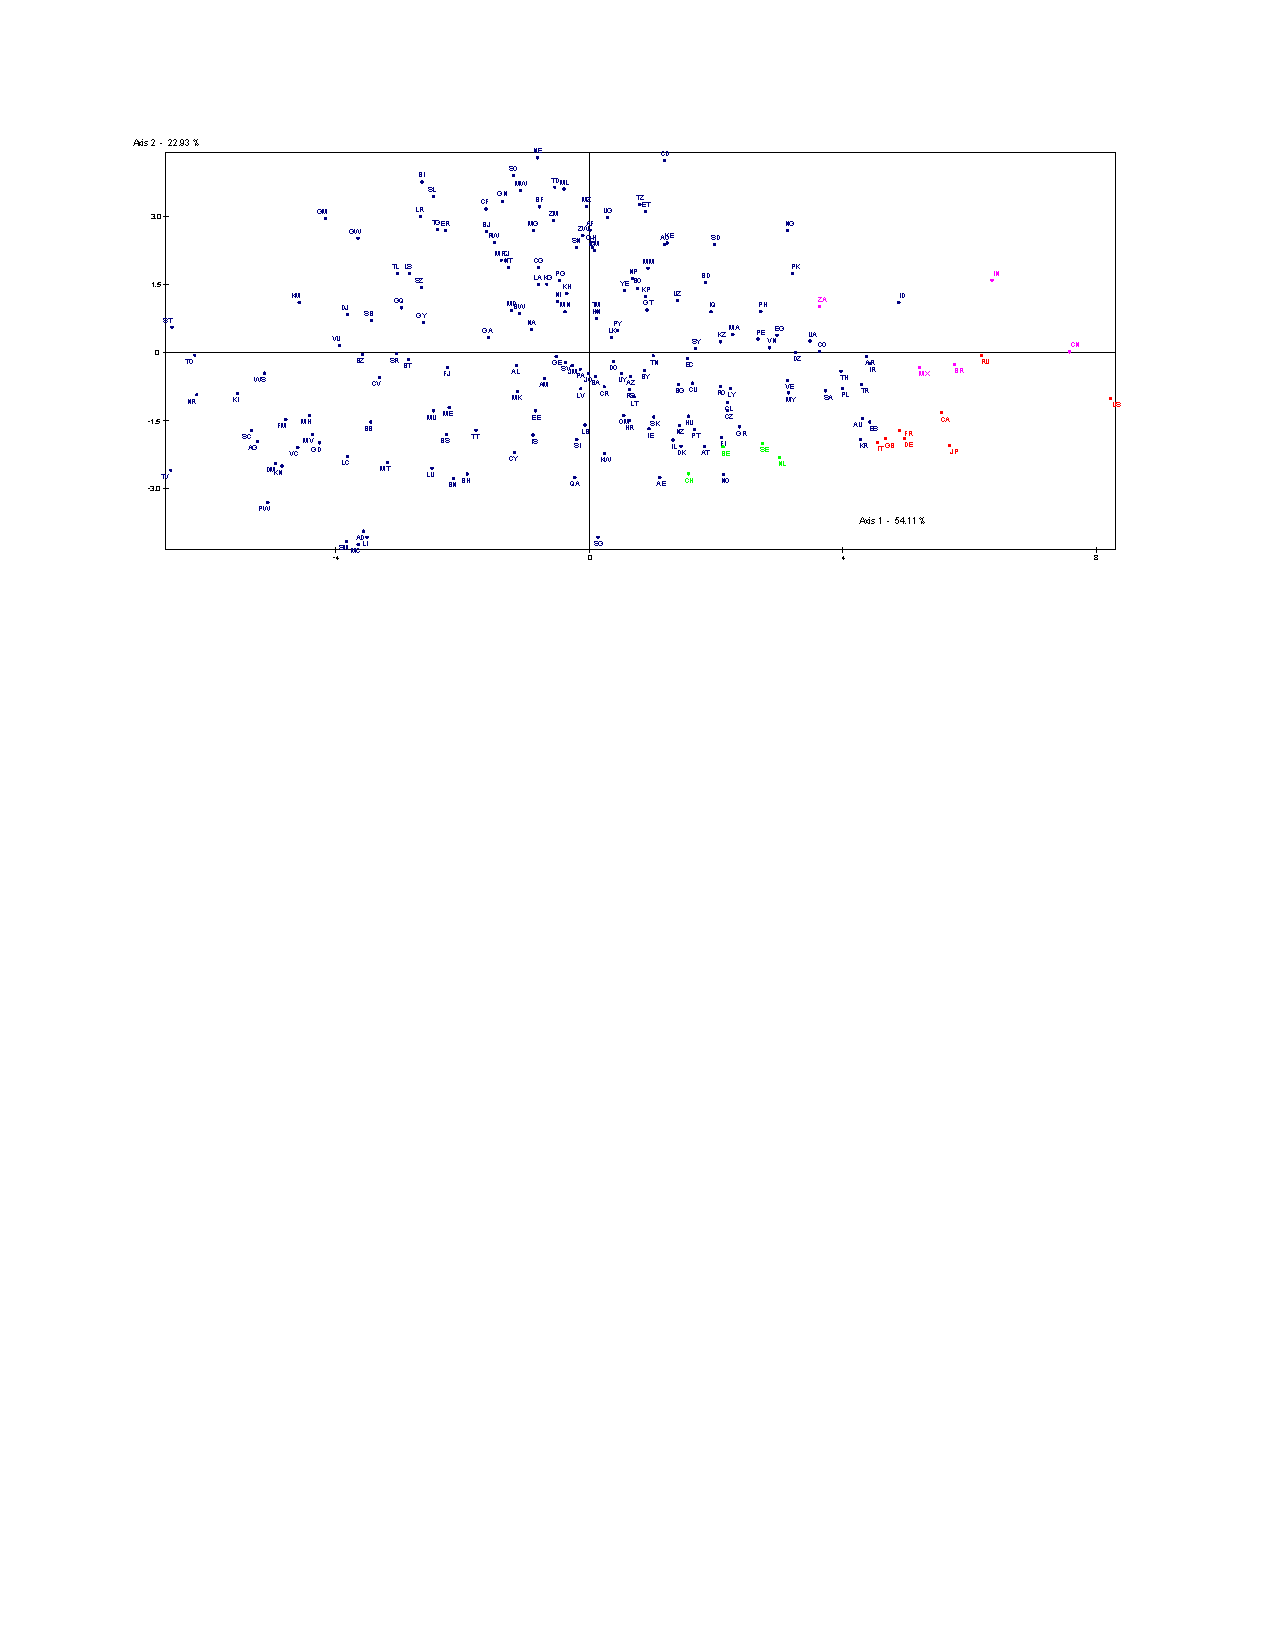
\includegraphics[width=17cm]{r1.pdf}
\caption{\footnotesize{Results of the normed PCA carried out on the selected  variables in the set.}\label{r1}}
\end{center}
\end{figure}


\begin{figure}[!ht]
\begin{center}
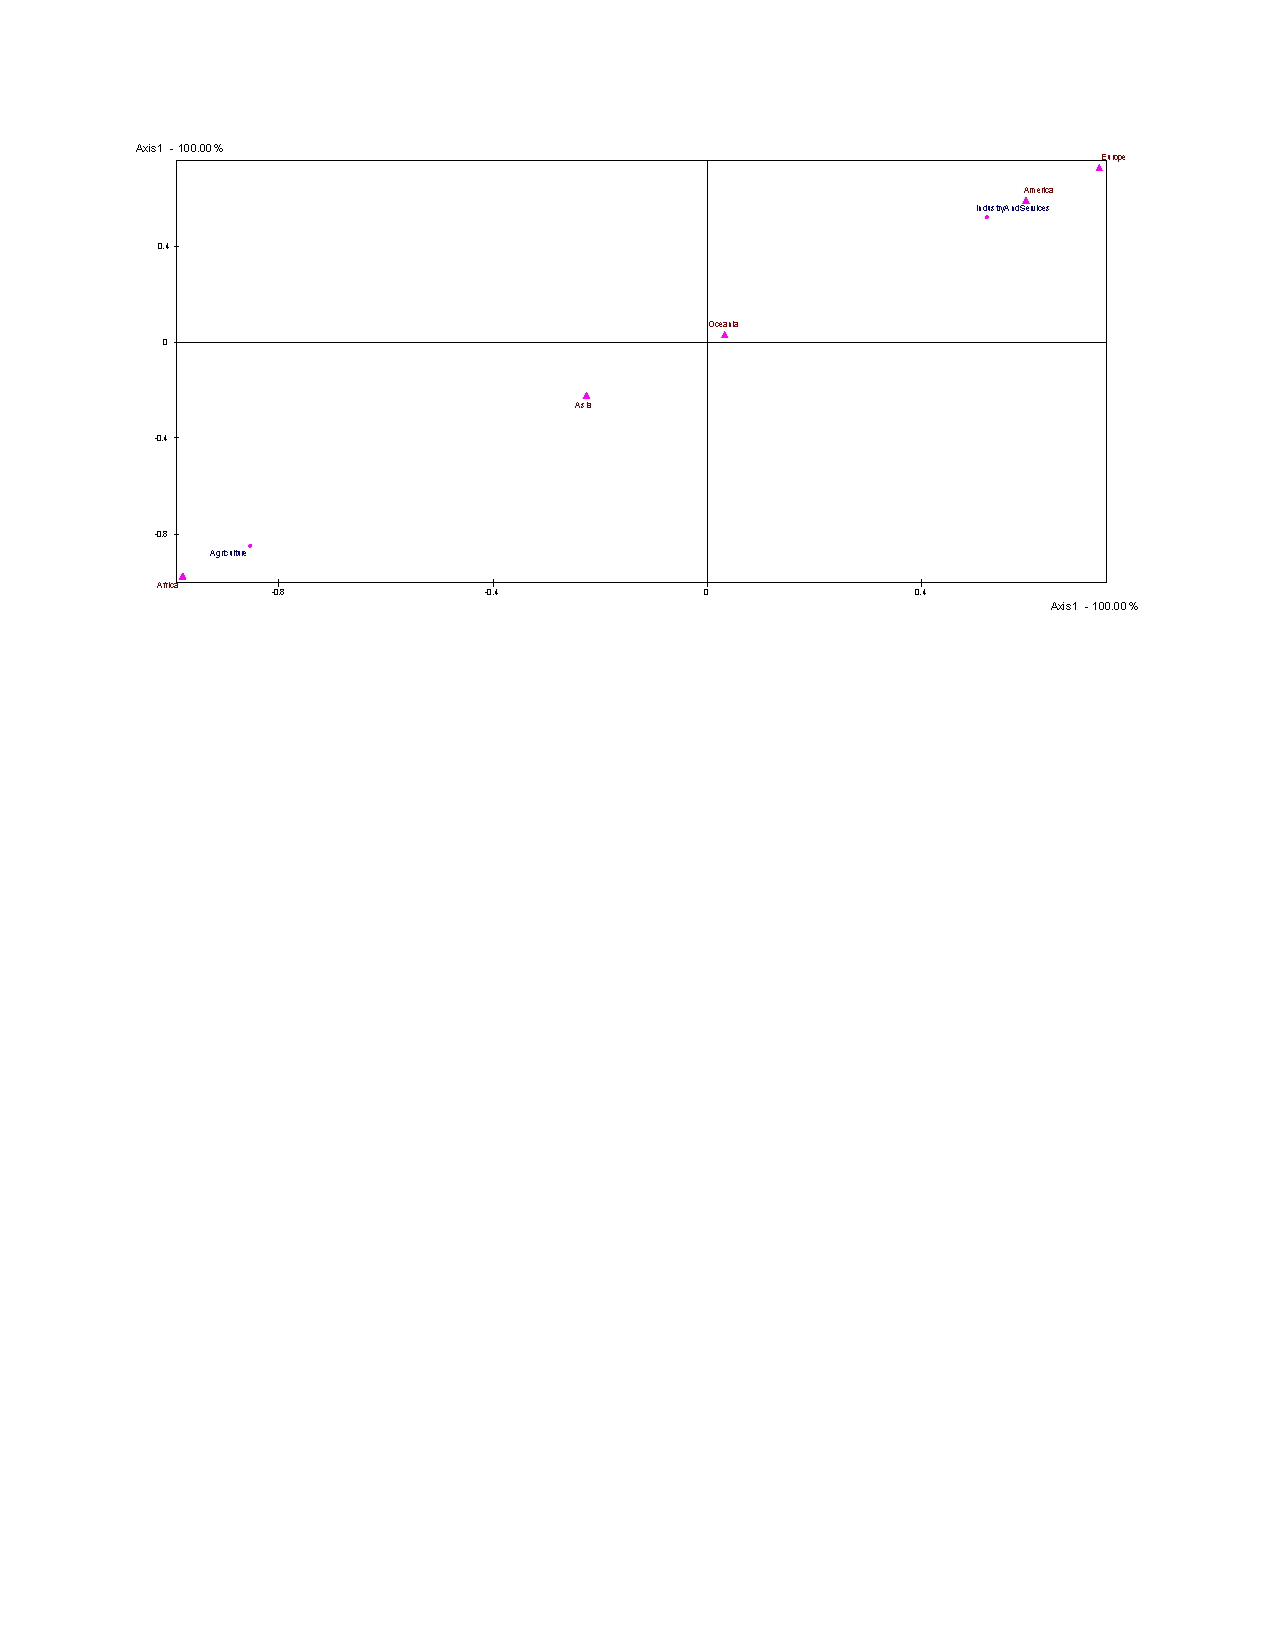
\includegraphics[width=17cm]{r2a.pdf}
\caption{\footnotesize{Results of the CA carried out on the selected variables in the set.}\label{r2}}
\end{center}
\end{figure}


\newpage


\end{document}